\documentclass[12pt, a4paper]{article}
\usepackage[utf8]{inputenc}
\usepackage{graphicx}
\usepackage{amsmath}
\usepackage{amssymb}
\usepackage{hyperref}
\usepackage{booktabs}
\usepackage{array}
%\usepackage{packages}
\usepackage{titlepage}
\usepackage[backend=biber, style=ieee]{biblatex}
\addbibresource{references.bib} 
\setlength{\parskip}{16pt}
\usepackage{float}
\usepackage{multicol}
\usepackage[margin=1.5cm]{geometry}

% Title page settings
\setToResearch
\setTitle{Innovative Approaches to Multi-User Tracking in Retail Spaces}
\setStageOne % Setting to first stage as shown in the image (interim, the first stage)
\setGroup{232}
\setStudentSgn{} % Student signature placeholder
\setStudent{Ivan Novosad}
\setStudentDate{}
\setAdvisor{Peter Lukianchenko}
\setAdvisorTitle{Head of the AI in Mathematical Finance Laboratory}
\setAdvisorAffiliation{Higher School of Economics, Department of Big Data}
\setAdvisorDate{}
\setGrade{}
\setAdvisorSgn{} % Advisor signature placeholder
\setYear{2025}


\begin{document}

\makeTitlePage

\begin{abstract}
This research details the development of an innovative system for continuous multi-user tracking within retail environments, focusing on robust single-camera tracking and effective cross-camera re-identification (Re-ID). A key contribution for single-camera tracking is the application of tailored post-processing heuristics addressing phantom tracks and manikin misclassifications to a state-of-the-art pipeline (YOLOv12, BoT-SORT, OSNet). The primary innovation lies in the cross-camera Re-ID methodology, which overcomes the limitations of appearance-only approaches in challenging retail settings. This is achieved through a robust spatiotemporal matching strategy utilizing homography to establish a common ground plane for coordinate-based comparisons. A novel exponential loss function is introduced for similarity scoring, significantly improving matching accuracy, particularly in scenarios with partial occlusions or non-ideal detections. The system architecture proposes a multi-stage matching process, where spatiotemporal constraints primarily guide Re-ID, with aggregated appearance features from multiple confirmed views providing a fallback mechanism, ensuring high accuracy and stability in generating comprehensive visitor trajectories.
\end{abstract}

\tableofcontents

\section{MOT pepiline}
\subsection{Problem formulation}

First of all we want to state MOT problem mathematically. Different works gives their own definitions, but the general one was given in \cite{lit-review}.

Multiple object tracking can be categorized as a problem of multi-variable estimation. For a given sequence of images, 
we denote $\mathbf{x}_k^j$ as the state of the $j$-th object in frame $k$, and 
$\mathbf{X}_k = (\mathbf{x}_k^1, \mathbf{x}_k^2, \ldots, \mathbf{x}_k^{N_k})$ to represent the states of all $N_k$ 
objects present in frame $k$. The sequential states of the $j$-th object are denoted by 
$\mathbf{x}_{a:b}^j = \{\mathbf{x}_{a}^j, \ldots, \mathbf{x}_{b}^j\}$, where $a$ and $b$ 
indicate the first and last frames in which object $j$ appears. Furthermore, $\mathbf{X}_{1:k} = \{\mathbf{X}_1, \mathbf{X}_2, \ldots, \mathbf{X}_k\}$ 
represents all sequential states of all objects from the initial frame through frame $k$. Note that the number of objects may be diffrent between frames.

In the Detection Based Tracking Frameworks, which is widely adopted in to solve MOT problem, 
we denote the measurements for the $j$-th object in frame $k$ as $\mathbf{z}_k^j$. The collection of all measurements 
in frame $k$ is represented as $\mathbf{Z}_k = (\mathbf{z}_k^1, \mathbf{z}_k^2, \ldots, \mathbf{z}_k^{N_k})$, while 
$\mathbf{Z}_{1:k} = \{\mathbf{Z}_1, \mathbf{Z}_2, \ldots, \mathbf{Z}_k\}$ encompasses all sequential measurements 
of all objects from the initial frame through frame $k$.

The fundamental goal of multiple object tracking is to determine the "optimal" sequential states for all objects. This can be 
formulated as a Maximum a posteriori (MAP) estimation problem based on the conditional probability distribution of the sequential 
states given all available measurements:
\begin{equation}
\mathbf{X}_{1:k}^* = \arg\max_{\mathbf{X}_{1:k}} p(\mathbf{X}_{1:k} | \mathbf{Z}_{1:k})
\end{equation}

There are two approaches to solve the above MAP problem, either from a \textbf{probabilistic inference} perspective or a
\textbf{deterministic optimization} perspective.

\subsection{Optimization methods}

As shown in this paper \cite{Inference_base} \textbf{The probabilistic inference based} approaches usually solve 
the MAP problem in Eq.~(1) using a two-step iterative procedure as follows:

\textbf{Predict:} $p(\mathbf{X}_k|\mathbf{Z}_{1:k-1}) = \int p(\mathbf{X}_k|\mathbf{X}_{k-1})p(\mathbf{X}_{k-1}|\mathbf{Z}_{1:k-1})d\mathbf{X}_{k-1}$,

\textbf{Update:} $p(\mathbf{X}_k|\mathbf{Z}_{1:k}) \propto p(\mathbf{Z}_k|\mathbf{X}_k)p(\mathbf{X}_k|\mathbf{Z}_{1:k-1})$.

Where: $p(\mathbf{X}_k|\mathbf{X}_{k-1})$ is \textit{Dynamic Model} and $p(\mathbf{Z}_k|\mathbf{X}_k)$ is  \textit{Observation Model}.

In contrast, \textbf{deterministic optimization} approaches tackle the problem by maximizing the likelihood 
function $L(\mathbf{Z}_{1:k}|\mathbf{X}_{1:k})$ which serves as a proxy for $p(\mathbf{X}_{1:k}|\mathbf{Z}_{1:k})$ across the collection of detected observations 
$\{\hat{\mathbf{Z}}^n_{1:k}\}$:

\begin{equation}
\mathbf{X}_{1:k}^* = \arg\max_{\mathbf{X}_{1:k}} p(\mathbf{X}_{1:k}|\mathbf{Z}_{1:k}) = \arg\max_{\mathbf{X}_{1:k}} L(\mathbf{Z}_{1:k}|\mathbf{X}_{1:k}) = \arg\max_{\mathbf{X}_{1:k}} \prod_n p(\hat{\mathbf{Z}}^n_{1:k}|\mathbf{X}_{1:k})
\end{equation}

Alternatively \cite{lit-review}, these approaches can be formulated as minimizing an energy function $E(\mathbf{X}_{1:k}|\mathbf{Z}_{1:k})$:

\begin{equation}
\mathbf{X}_{1:k}^* = \arg\max_{\mathbf{X}_{1:k}} p(\mathbf{X}_{1:k}|\mathbf{Z}_{1:k}) = \arg\max_{\mathbf{X}_{1:k}} \frac{\exp(-E(\mathbf{X}_{1:k}|\mathbf{Z}_{1:k}))}{Z} = \arg\min_{\mathbf{X}_{1:k}} E(\mathbf{X}_{1:k}|\mathbf{Z}_{1:k}),
\end{equation}

where $Z$ represents a normalization constant that ensures that $p(\mathbf{X}_{1:k}|\mathbf{Z}_{1:k})$ maintains the properties of a valid probability distribution.

\subsection{Initialization Methods}
There are two  widely used approaches of how to initialize objects: Detection-Based Tracking (DBT) (picture \ref{fig:dftdbt} on the left) and Detection-Free Tracking (DFT)[\cite{DFT_pipe}] (picture \ref{fig:dftdbt} on the right )

\begin{figure}[h]
    \centering
    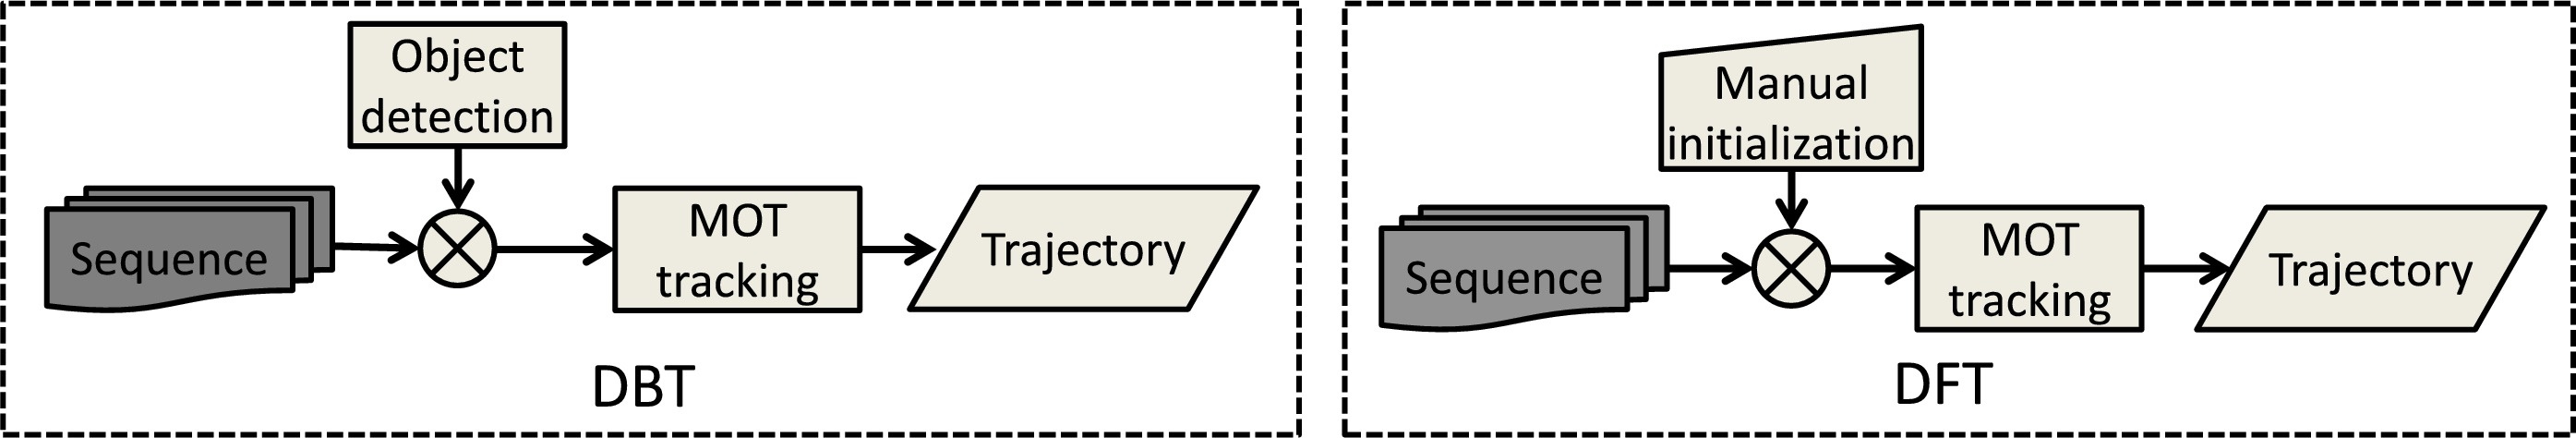
\includegraphics[width=0.95\linewidth]{pictures/DBT_DFT.jpg}
    \caption{Detection based vs Detection free tracking}
    \label{fig:dftdbt}
\end{figure}

\textbf{Detection-free Tracking (DFT)} - requires manual initialization of a fixed number of objects in the first frame, 
then localities these objects in subsequent frames.  Despite the higher accuracy of the tracking compared to DBT, it is impossible to use this method within the set task because the number of people in the frame is constantly varying.

\textbf{Detection-based Tracking (DBT)} - objects first detected by the detection model and then linked into trajectories. Using the object detection model we identify targets (bounding boxes) in each video frame and then we use data association for link these detections across frames to form continuous trajectories.

\subsection{Detection Model}

In this work \cite{detectionModelsSurvey} authors list all milestone object detection models. They split the progress of object detection 
into two historical periods: the “traditional object detection period (before 2014)” and the “deep learning-based detection period (after 2014). 
A review of traditional models is beyond the scope of this article, so let's take a look at modern approaches. Authors consider two main approaches: 

\paragraph{Two-Stage Detectors}
One of the most efficient and popular architecture is R-CNN. Original R-CNN \cite{rcnn} used Selective Search \cite{selective_serach} for region proposals followed by independent CNN processing (pipeline shown in Fig.~\ref{fig:rcc_pipe}), achieving accuracy but with extreme inefficiency (48h training with 58.5\% mAP on VOC07 \cite{voc07}). Fast R-CNN \cite{fastRCNN} introduced RoI pooling on shared feature maps (shown in Fig.~\ref{fig:frcc_pipe}), reducing training time to 9h while maintaining 65\% mAP on VOC07. Faster R-CNN \cite{fasterRCNN} completed the evolution by replacing Selective Search with a learnable Region Proposal Network (RPN) (Fig.~\ref{fig:faster_rcnn}), enabling end-to-end training and near-real-time detection (5 FPS).

\begin{figure}[h]
\begin{minipage}[t]{0.55\textwidth}
    \begin{figure}[H]
        \centering
        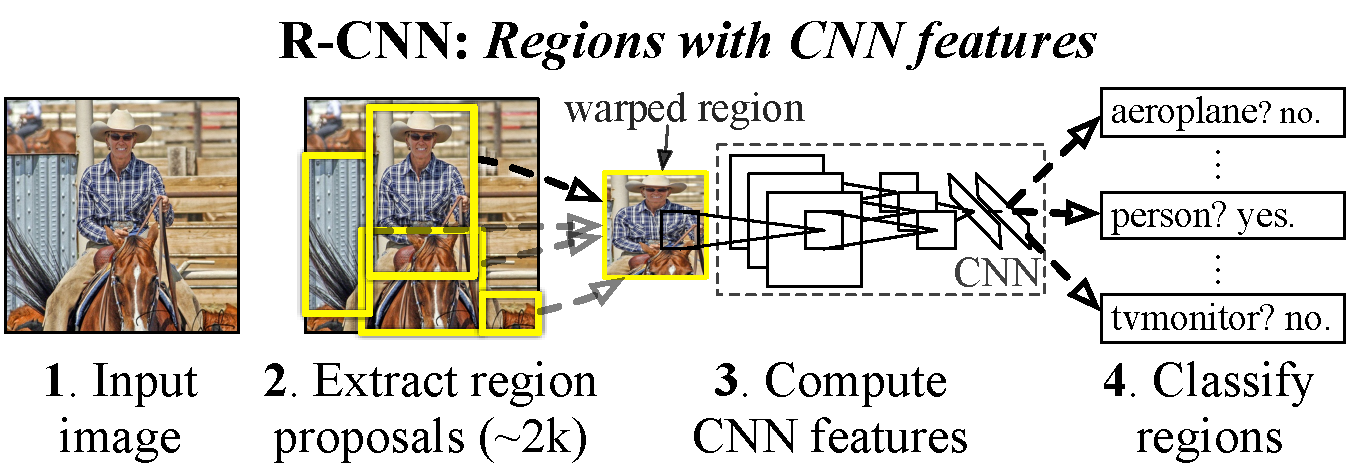
\includegraphics[width=\linewidth]{pictures/rcc_pipe.pdf}
        \caption{R-CNN pipeline}
        \label{fig:rcc_pipe}
    \end{figure}
    
    \begin{figure}[H]
        \centering
        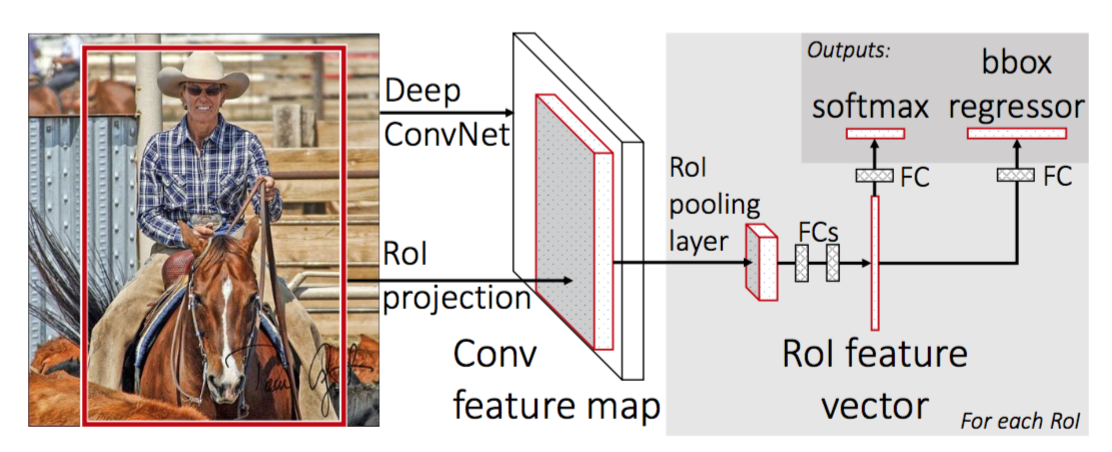
\includegraphics[width=\linewidth]{pictures/frcnn.png}
        \caption{Fast R-CNN RoI}
        \label{fig:frcc_pipe}
    \end{figure}
\end{minipage}
\hfill
\begin{minipage}[t]{0.4\textwidth}
    \begin{figure}[H]
        \centering
        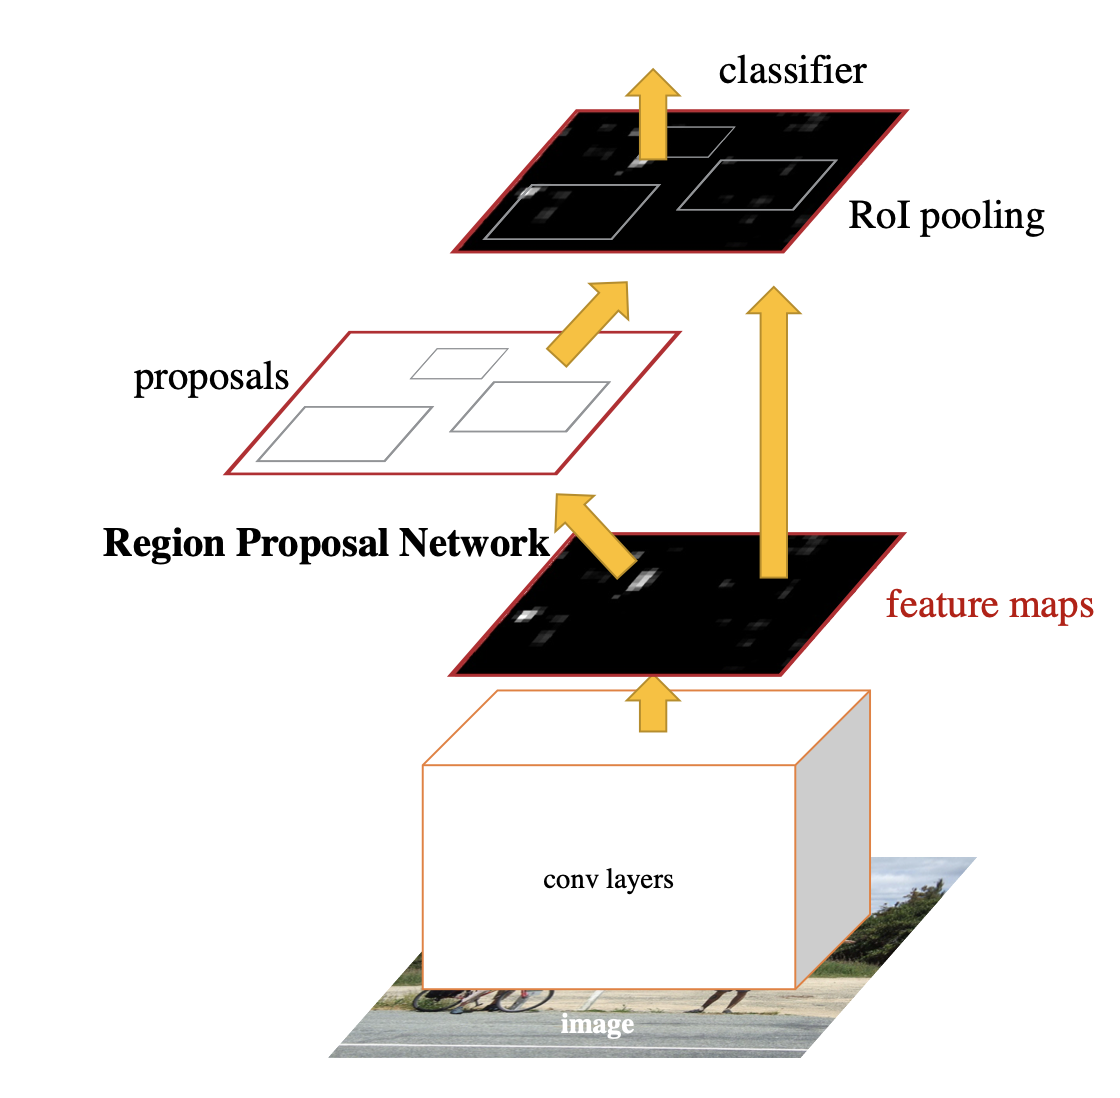
\includegraphics[width=\linewidth]{pictures/faster_rcnn.png}
        \caption{Faster R-CNN Features and proposal extraction pipeline}
        \label{fig:faster_rcnn}
    \end{figure}
\end{minipage}
\end{figure}

\paragraph{One-Stage Detectors}
\emph{}
YOLO (You Only Look Once) initially proposed in 2015 \cite{yolov1}. Firstly, given image is divided into an $S \times S$ grid,
where each grid cell is responsible for detecting objects whose center falls within it. 
Each grid cell predicts $B$ bounding boxes and confidence scores for those boxes. Intuitively, these confidence scores reflect how confident 
the model is that the box contains an object and also how accurate it thinks the box is that is predicts. Formally, it's define confidence as 
$\Pr(\text{Object}) * \text{IOU}_{\text{pred}}^{\text{truth}}$. If no object exists in that cell, the confidence scores should be zero. Otherwise we want the confidence score to equal the intersection over union (IOU) between the predicted box and the ground truth.

\begin{figure}[h]
    \centering
    \begin{minipage}{0.45\textwidth}
        \centering
        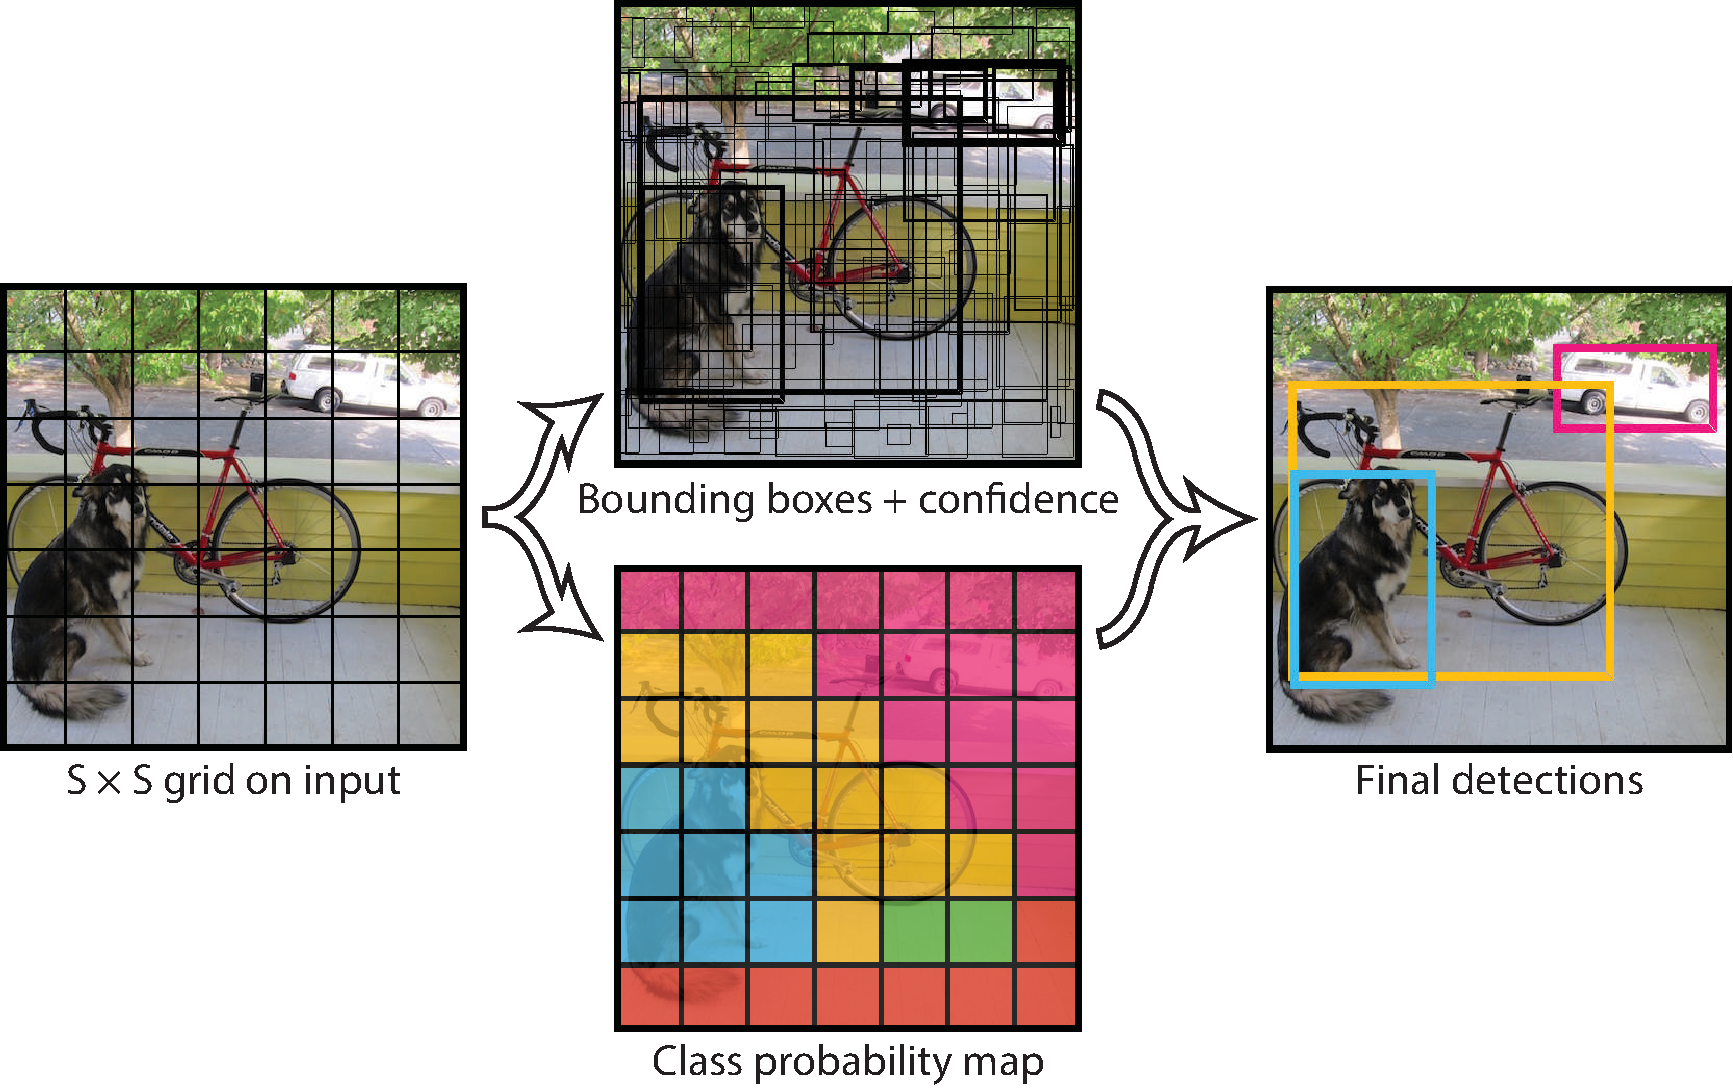
\includegraphics[width=\linewidth]{pictures/yolov1_dog.pdf}
        \caption{YOLOv1 detection pipeline}
        \label{fig:yolov1_dog}
    \end{minipage}
    \hfill
    \begin{minipage}{0.45\textwidth}
        \centering
        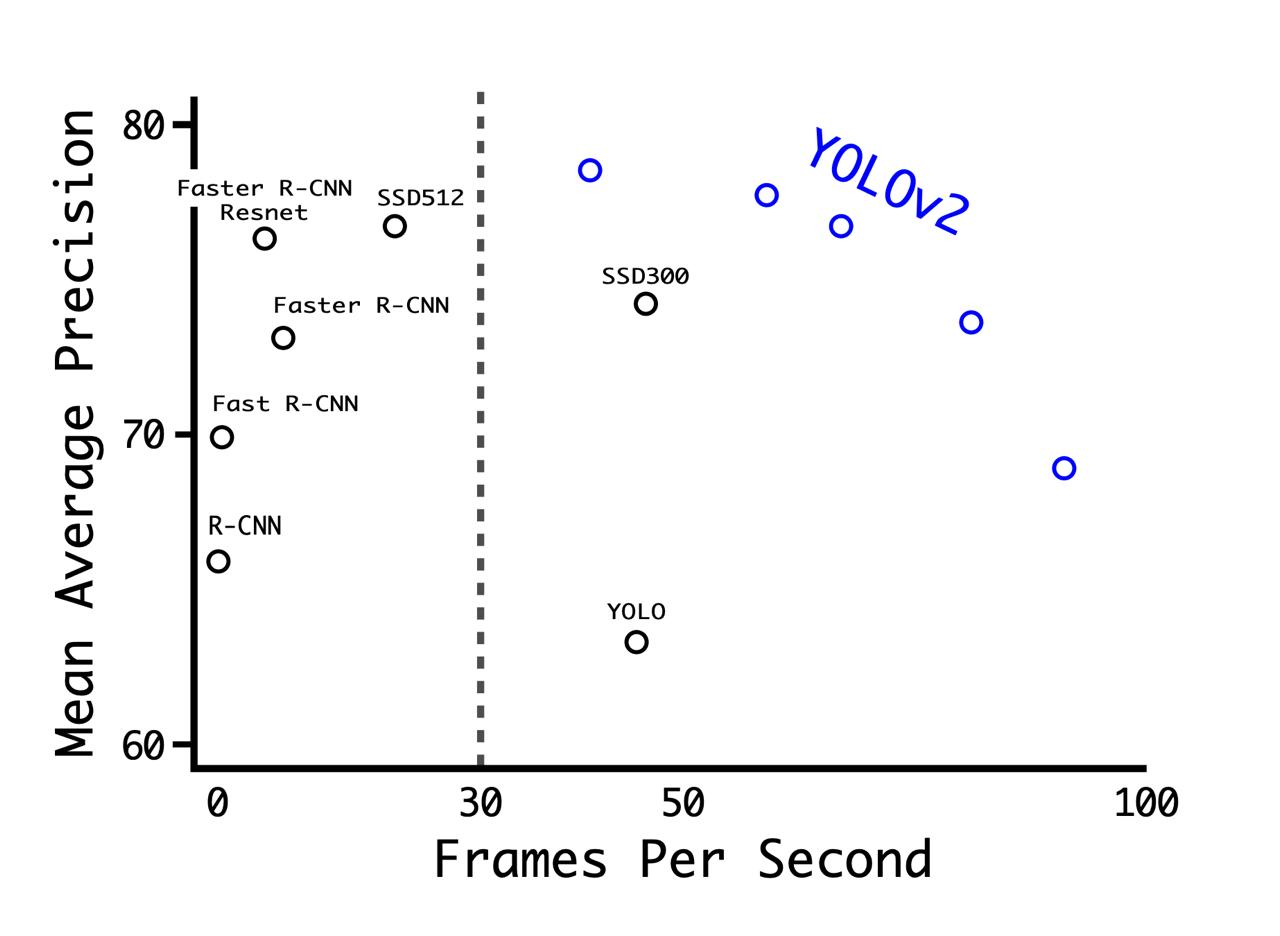
\includegraphics[width=\linewidth]{pictures/yolov2.jpeg}
        \caption{Accuracy/speed comparison on VOC07}
        \label{fig:yolov2}
    \end{minipage}
\end{figure}

YOLOv2 \cite{yolov2} significantly improved upon this architecture in 2017 by introducing Darknet-19 backbone 
(which can classify 9000 objects types) with batch normalization, 
Anchor boxes, dimension clusters and VGG-inspired data augmentation \cite{vgg}.
These enhancements yielded both speed and accuracy improvements as shown in Figure~\ref{fig:yolov2}.

YOLOv3 \cite{yolov3} improves upon YOLOv2 with three key improvements: features extraction changed to Darknet-53 that incorporates residual connections, using a Feature Pyramid Network \cite{featurepyramidnetwork} to predict multi-scale bounding boxes to better detection of objects of various size, change the softmax to independent logistic classifier for handling overlapping labels

YOLOv4 \cite{yolov4} significantly improves upon YOLOv3 ~\ref{fig:yolov4} by introducing a more efficient backbone (CSPDarknet53 instead of Darknet53), incorporating additional modules like SPP (Spatial Pyramid Pooling) and PAN (Path Aggregation Network) \cite{PAN} in the neck, and implementing numerous training enhancements which authors categorized as "Bag of Freebies" (I'm not joking, that's a cite) (including Mosaic data augmentation, CIoU loss, and DropBlock regularization) and "Bag of Specials" (including Mish activation and DIoU-NMS).

\begin{figure}[h]
    \centering
    \begin{minipage}{0.45\textwidth}
        \centering
        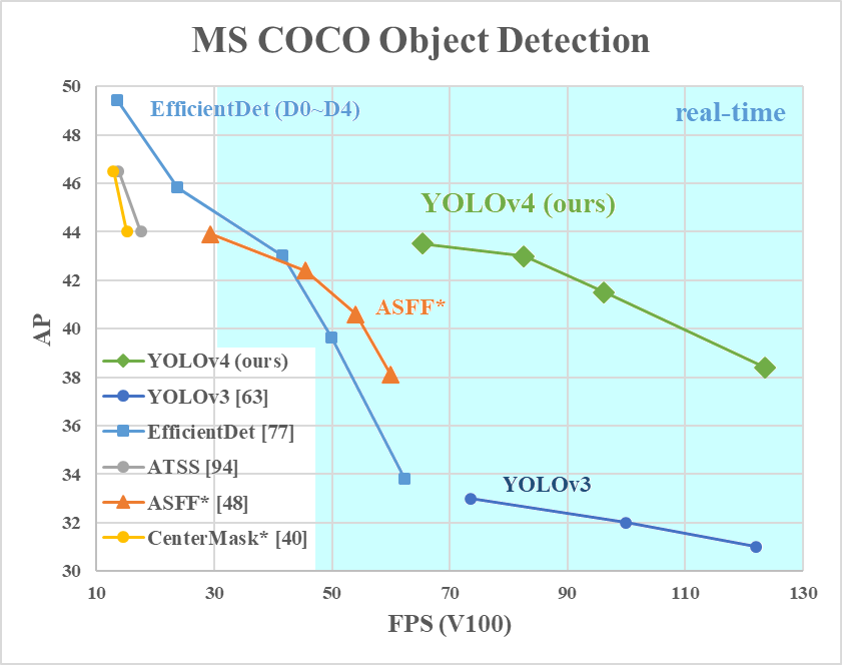
\includegraphics[width=\linewidth]{pictures/yolov4.png}
        \caption{Comparison of the proposed YOLOv4 with YOLOv3 and other SOTA (in 2020) models}
        \label{fig:yolov4}
    \end{minipage}
    \hfill
    \begin{minipage}{0.45\textwidth}
        \centering
        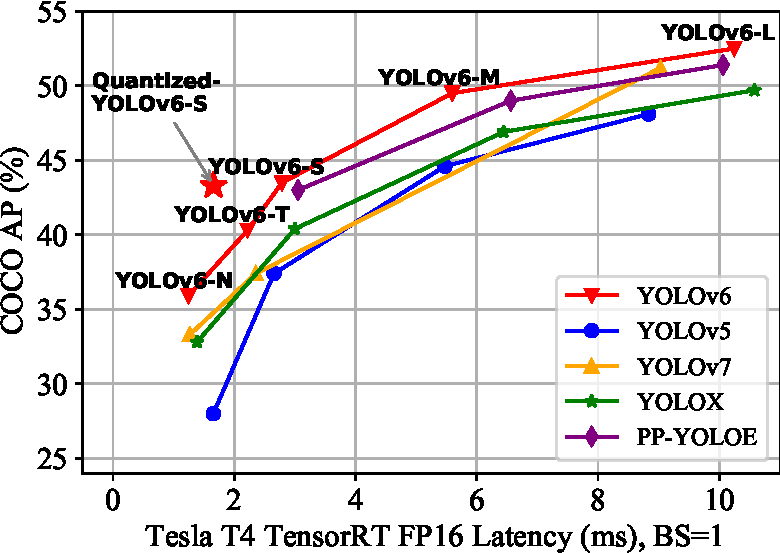
\includegraphics[width=\linewidth]{pictures/yolov6.pdf}
        \caption{Comparison of YOLO models on COCO}
        \label{fig:yolov6}
    \end{minipage}
\end{figure}

YOLOv5 \cite{yolov5} was first model designed by side authors (Ultralytics). Main difference from YOLOv4 is native PyTorch implementation (moving away from v4’s Darknet C framework). YOLOv5 introduces refinements such as Focus layer and auto-learning bounding box anchors. 

YOLOv6 \cite{yolov6} redesign backbone using RepVGG-style blocks for small models and CSPStackRep blocks for larger ones. YOLOv6 also adopts an anchor-free approach with a decoupled head using a hybrid-channel strategy. Also new training techniques was used: Task Alignment Learning (TAL) for label assignment, VariFocal Loss for classification, and self-distillation for both classification and regression tasks. 

YOLOv7's \cite{yolov7} architecture main features the Extended Efficient Layer Aggregation Network (E-ELAN). It uses group convolution which allows to increase cardinality saving the original gradient path. For re-scaling model YOLOv7 uses novel compund scaling method which specifically designed for concatenation-based models. On the training side, authors intoroduces (cite) "trainable bag-of-freebies", planned re-parameterized convolution that applies RepConv based on gradient flow analysis. 

YOLOv8 \cite{yolov8}, developed by Ultralytics, advances beyond YOLOv5 (previous models of Ultralytics) by adopting anchor-free detection mechanism (as was initially introduced in YOLOv7) and introducing a new CSP-based backbone (e.g., with C2f modules replacing C3 modules). Also training methods was taken from YOLOv7 and authors uses Distribution Focal Loss in training process.

\begin{figure}[h]
    \centering
    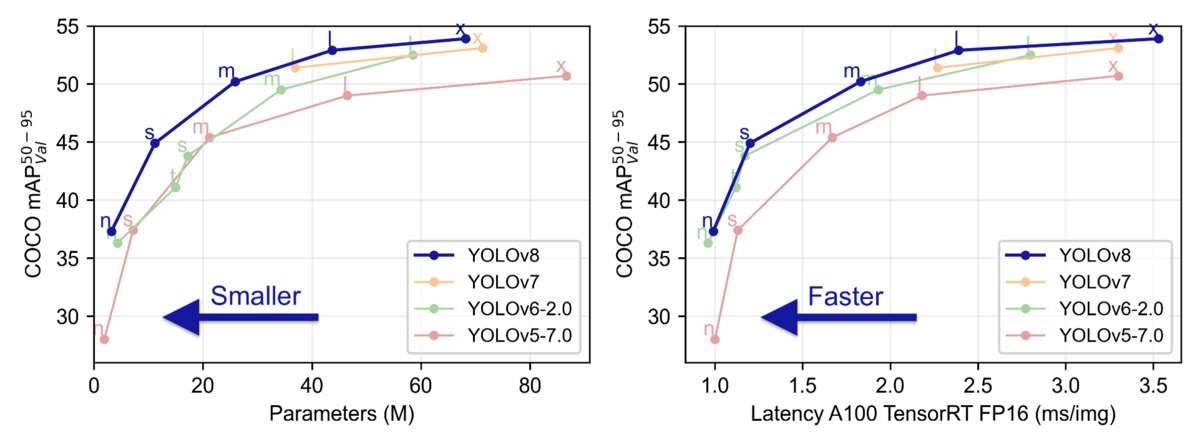
\includegraphics[width=0.95\linewidth]{pictures/yolov8.png}
    \caption{Comparison of YOLOv8 against v7 and previous v5 models}
    \label{fig:yolov8}
\end{figure}

YOLOv9 \cite{yolov9} introduces two fundamental architectural innovations: Programmable Gradient Information (PGI) and Generalized Efficient Layer Aggregation Network (GELAN). YOLOv9 tackles "the information bottleneck" problem through PGI's branch that preserves backpropagation and generates more gradients during training (not used on inference, therefore don't add inference cost). Meanwhile, GELAN extends YOLOv7's ELAN architecture by generalizing it to support arbitrary computational blocks. GELAN achieves higher parameter utilization than depth-wise convolution. 

YOLOv10 \cite{yolov10} introduces two different architectural concepts in addition to the YOLOv9 architecture.
First: "consistent dual assignments" eliminates the need for Non-Maximum Suppression (NMS). This approach uses parallel one-to-many and one-to-one heads during training, while during inference only the one-to-one head is used, providing full end-to-end deployment.
Second, YOLOv10 implements a "holistic efficiency-accuracy driven model design". This includes a new classification head, spatial-channel decoupled downsampling, and rank-guided block design that adaptively uses compact inverted blocks (CIB). For smaller models, YOLOv10 uses convolutions with larger kernels. The authors also introduce a partial self-attention (PSA) module (partial because it processes only a portion of the feature channels).

YOLOv11 \cite{yolov11} builds upon YOLOv10 by introducing the C3k2 (Cross Stage Partial with kernel size 2) block, which replaces previous C2f blocks for computational efficiency by using two smaller convolutions. (There are some works what proves imperially what several smaller kernels takes an advantage on few larger convolutions). It also incorporates a C2PSA (Convolutional block with Parallel Spatial Attention) component after the SPPF block to improve spatial attention. Additionally, YOLOv11 add explicit support for oriented object detection (OBB) as a core task.

\begin{figure}[h]
    \centering
    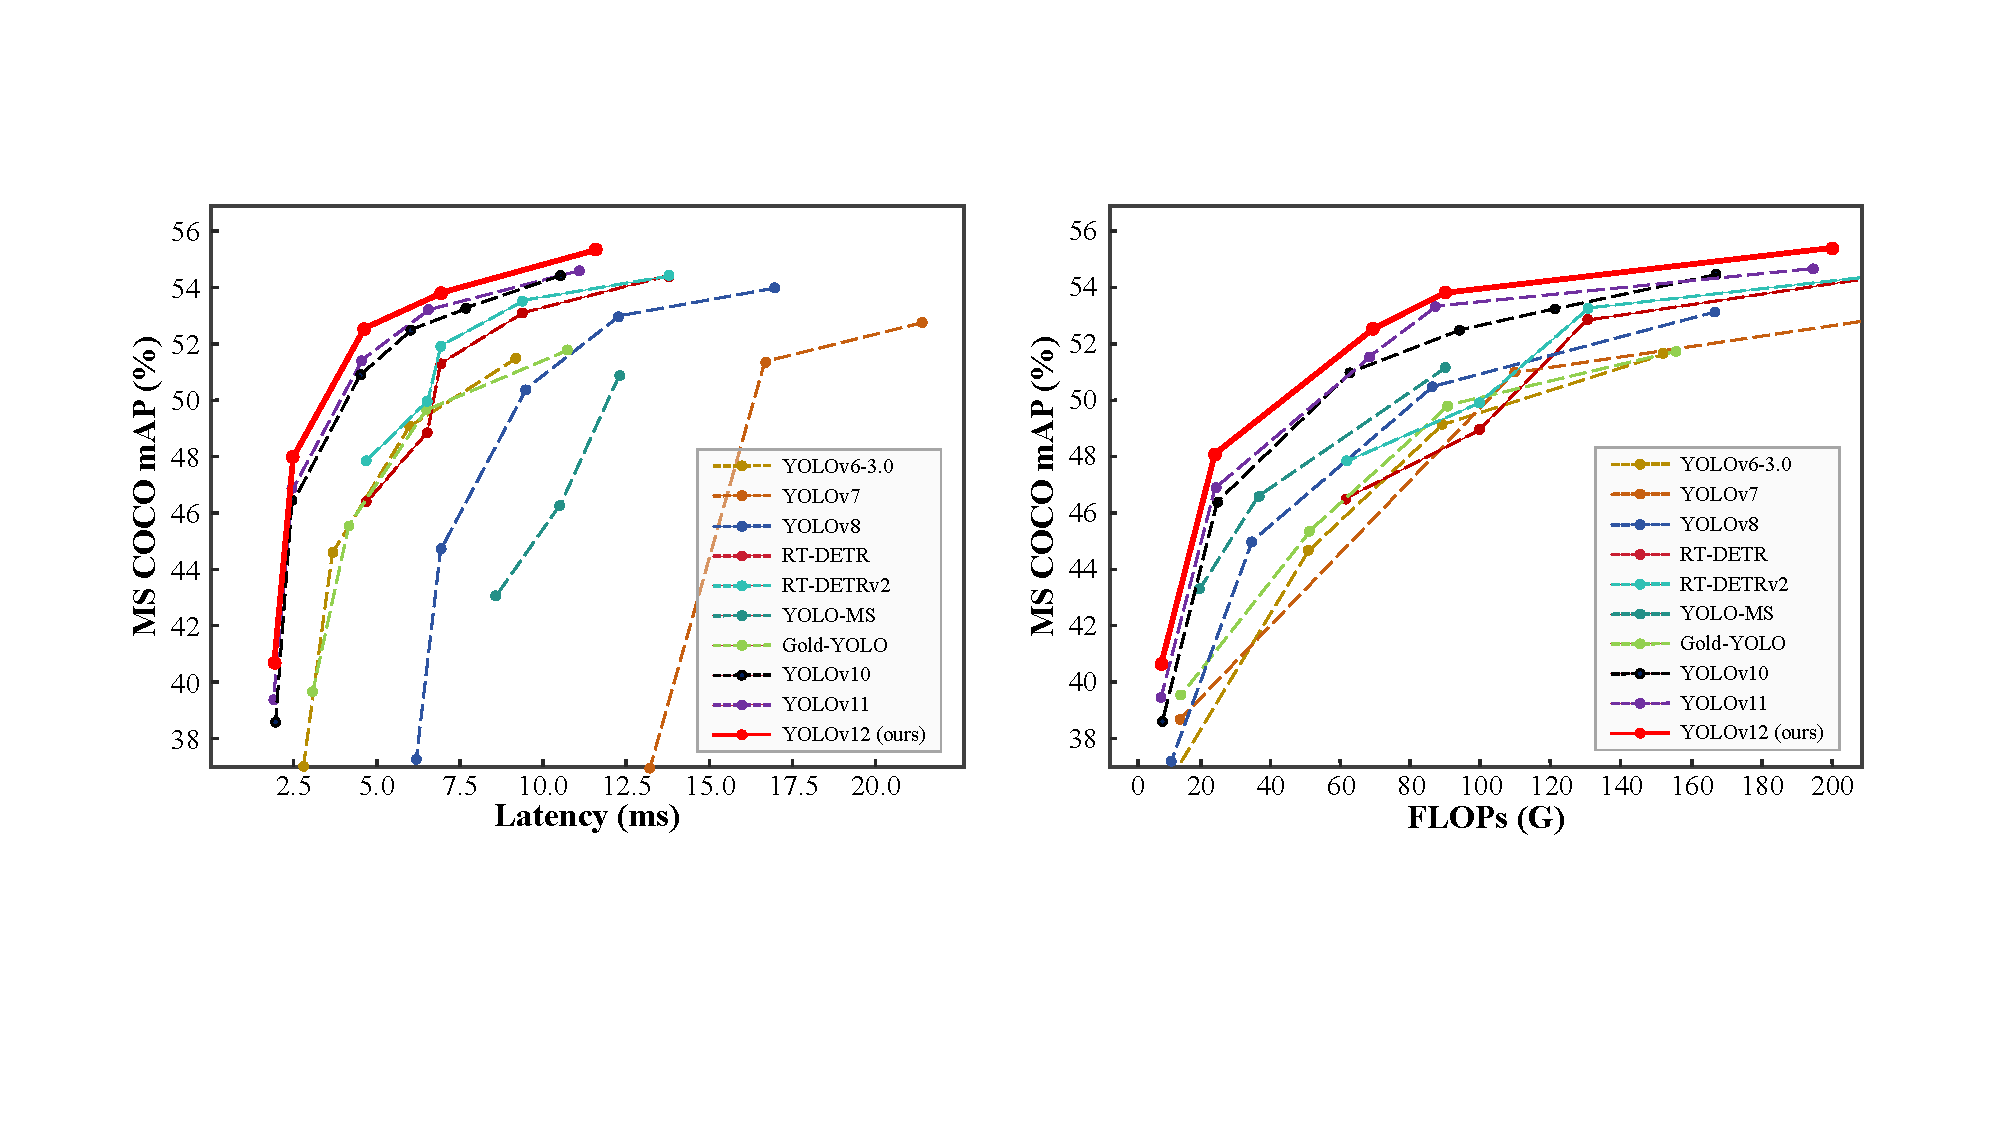
\includegraphics[width=0.95\linewidth]{pictures/yolov12.pdf}
    \caption{SOTA YOLOv12 compared to previous versions}
    \label{fig:yolov12}
\end{figure}

YOLOv12 \cite{yolov12} represents a significant architectural shift from YOLOv11 by introducing an attention-centric framework. The key innovation is the Area Attention (A2) module, which divides feature maps into equal vertical or horizontal segments to reduce computational complexity while preserving large receptive fields. YOLOv12 also introduces Residual Efficient Layer Aggregation Networks (R-ELAN), which enhances the original ELAN architecture with block-level residual connections and scaling techniques. The architecture removes traditional components like positional encoding for efficiency and replaces them with a position perceiver using large separable convolutions (7×7). YOLOv12 incorporates FlashAttention to overcome memory access inefficiencies inherent in attention mechanisms and adjusts the MLP ratio from 4 to 1.2 (or 2 for smaller models) to better balance computational resources. Unlike previous YOLO versions that relied primarily on CNN-based improvements, YOLOv12 uses attention mechanisms into the YOLO framework.


\subsection{Comparison of Object Detection Paradigms}


\begin{table}[]
\centering
\caption{Comparison of DeepLearning Object Detection Paradigms}
\begin{tabular}{|>{\raggedright\arraybackslash}m{2.5cm}|>{\raggedright\arraybackslash}m{4cm}|>{\raggedright\arraybackslash}m{3.5cm}|>{\raggedright\arraybackslash}m{4.5cm}|>{\raggedright\arraybackslash}m{3cm}|}
\hline
\textbf{Paradigm} & \textbf{Key Characteristics} & \textbf{Strengths} & \textbf{Challenges/Limitations} & \textbf{Performance Examples} \\
\hline
\textbf{Two-Stage Detectors (R-CNN)} & Region proposals followed by CNN classification; evolved from R-CNN to Faster R-CNN with RPN. & High accuracy; end-to-end training (Faster R-CNN); robust for complex scenes. & High computational cost; slow inference (e.g., R-CNN: 48h training); complex pipeline. & R-CNN: 58.5\% mAP (VOC07), Fast R-CNN: 65\% mAP (VOC07), Faster R-CNN: 5 FPS. \\
\hline
\textbf{One-Stage Detectors (YOLO)} & Single-pass prediction of bounding boxes and classes; grid-based (YOLOv1) to advanced backbones (YOLOv12). & Fast inference; real-time applicability; improving accuracy with versions. & Lower accuracy than two-stage in early versions; struggles with small objects, crowded scenes. & YOLOv1: 63.4\% mAP (VOC07), YOLOv12: SOTA on COCO (2025). \\
\hline
\textbf{Anchor-Based Detectors} & Uses predefined anchor boxes for bounding box prediction (e.g., YOLOv2-v5, Faster R-CNN). & Effective for diverse object sizes; robust in structured scenes. & Sensitive to anchor design; struggles with extreme aspect ratios or dense scenes. & YOLOv4: 43.5\% AP (COCO), Faster R-CNN: 36.2\% AP (COCO). \\
\hline
\textbf{Anchor-Free Detectors} & Predicts object centers or keypoints directly (e.g., YOLOv6-v12, CornerNet). & Simplified pipeline; better for irregular shapes; reduced hyperparameter tuning. & May struggle with small objects; newer paradigm with less optimization in early models. & YOLOv6: 50.0\% AP (COCO), YOLOv12: Improved AP over YOLOv11 (COCO). \\
\hline
\label{detectionModelTable}
\end{tabular}
\end{table}

\paragraph{}
\begin{itemize}
    \item \textbf{Two-Stage}: Excels in accuracy computationally expensive;
    \item \textbf{One-Stage}: Prioritizes speed, with YOLOv12 introducing attention mechanisms for improved accuracy.
    \item \textbf{Anchor-Based}: Reliable but sensitive to anchor configuration; widely used in earlier YOLO and R-CNN models.
    \item \textbf{Anchor-Free}: Axcels anchor-based aproach; in newer YOLO versions (v6-v12).
\end{itemize}


\section{Tracking Model} 

According to this survey \cite{sota-trackets-survey} there are several key concepts in MOT (a.k. Categories):

\begin{enumerate}
	\item Separate detection and embedding (SDE) 
	\item Joint detection and embedding (JDE) 
	\item Tracking by regression 
	\item Tracking by attention 
\end{enumerate}
 

\subsection{The Separate Detection and Embedding (SDE) Paradigm}
\label{sec:Separate_Detection_Embedding}

The Separate Detection and Embedding (SDE) paradigm treats object detection and feature embedding for re-identification (ReID) as distinct tasks. This allows independent optimization of each component. This approach is divided into offline and online methods Fig. ~\ref{fig:online_offline}. 

\begin{figure}[h]
    \centering
    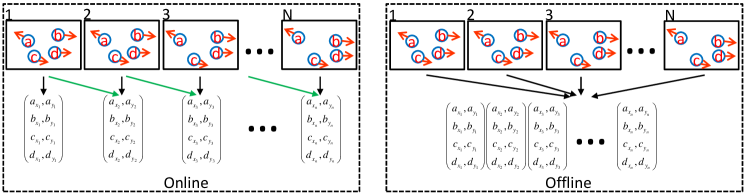
\includegraphics[width=0.95\linewidth]{pictures/online_offline.png}
    \caption{Online vs Offline MOT processing}
    \label{fig:online_offline}
\end{figure}

\paragraph{Offline SDE Methods:}
Offline tracking utilizes a batch of frames to process the data. As shown at Fig. \ref{fig:online_offline} (right) observations from the further frames used to proceed each frame, analyzing past and next frames  jointly to estimate the final output. Due to computational and memory limitation, it is not always possible to handle all the frames at once. An alternative solution is to split data into shorter video clips, and infer the results hierarchically or sequentially for each batch, or use a "sliding window" approach. 

Early methods like Joint Probabilistic Data Association (JPDA) \cite{JPDA}, Markov Chain Monte Carlo Data Association (MCMCDA) \cite{MCMCDA} and Multiple Hypothesis Tracking (MHT) \cite{MHT} potential trajectories by evaluation of feasible associations. Despite being quite accurate for the time, these methods are extremely difficult in a computational sense. To address this, graph optimization-based techniques \cite{global-data-association-using-network-flows, min-cost-network-flows, k-shortest-paths-for-mot, linear-programming-in-MOT} have been adapted and applied for modeling positional relationships and feature similarities between targets. For instance, network flow methods \cite{global-data-association-using-network-flows, min-cost-network-flows} formulate tracking as a min-cost flow problem (for crowded scenes). Similarly, k-shortest paths optimization \cite{k-shortest-paths-for-mot} and linear programming \cite{linear-programming-in-MOT} provide efficient solutions for large-scale (non crowded) tracking. Some heuristics of globally-optimal greedy algorithms \cite{global-optimal-greedy}
provide a balance between this two techniques, balancing accuracy and computational cost. Hierarchical schemes, such as the GMCP-tracker \cite{GMCP-tracker}, use generalized minimum clique graphs(complex interactions handling) and tracklet association with online target-specific metric learning \cite{target-specific-metric-learning}, it improves accuracy in crowded scenes. 

More recent advancements include conditional random fields (CRF) \cite{conditional-random-fields} for end-to-end learning, maximum-weight independent sets \cite{max-weight-set} for conflict resolution, spatio-temporal point processes \cite{Spatio-Temporal-Point-Process} for dynamic target modeling, box-plane matching [110] for dense scenes, and network flow for tracking-by-counting in crowd density maps \cite{Tracking-by-Counting}.

These methods well performing in scenarios with high occlusion and similar Appearance targets, however they are limited by their reliance on global information, making them impractical for real-time applications.

\paragraph{Online SDE Methods:}
Online methods, designed for real-time tracking associate detections with existing trajectories using only current and past frame information. This approach allows to run them in-time, also this significantly reducing the computational cost comparing this offline processing.

Early methods like SORT \cite{SORT} employ two-stage detectors such as Faster R-CNN, relying on Intersection over Union (IoU) for associating detections. This approach struggled with occlusions and leads to frequent identity switches (IDSW). To address this, DeepSORT \cite{DeepSORT} introduced a cascade matching scheme and deep learning-based appearance features, significantly reducing IDSW (from 1423 to 781 on MOT16) and improving MOTA from 59.8\% to 61.4\% \cite{DeepSORT}. 

Later, advantages of one-stage detectors, such as YOLO, have been integrated into DeepSORT. This leads to significant improvement in specific scenarios like intelligent transportation \cite{meimetis2021real}, nighttime traffic \cite{hu2023nighttime}, and aerial views from UAVs \cite{kapania2020multi}. The concept of anchor-free object detection was pioneered in CornerNet: Detecting Objects as Paired Keypoints \cite{CornerNet_anchor_free_origin}, having undergone minor transformations this approach was used in yolo models since version 6. This leads to further improvement of MOT systems. For instance, ByteTrack \cite{ByteTrack} improve tracking accuracy by incorporating low-scoring detections also, achieving MOTA scores of 80.3\% and 77.8\% on MOT17 and MOT20, respectively. BoT-SORT \cite{BoTsort} and StrongSORT \cite{StrongSORT} integrate motion and appearance cues. In fact, StrongSORT employ an appearance-free linking model (AFLink) and Gaussian Smoothed Interpolation (GSI) archiving trajectory continuity. OC-SORT \cite{os-sort} and its enhanced version, DEEP OC-SORT \cite{deep-os-sort} optimize Kalman filtering and employing appearance information (features) to recover lost trajectories in occlusion-heavy scenarios, while GHOST \cite{GHOST} improves appearance similarity modeling. In C-BIoU \cite{C-BIoU} the authors proposed to extend the bounding boxes during matching (if it's fails with smaller ones) to improve association success rates, particularly in crowded scenes. The POI tracker \cite{poi-tracker} employ skip pooling and multi-region modeling to combine features at different scales. Recurrent autoregressive networks \cite{recurrent-autoregressive-networks} measure appearance and motion states across frames, enabling better handling of non-linear motion Fig. ~\ref{fig:motion_linera_non_linear}. Tensor-based high-order graph matching \cite{tensor-based-high-order-graph-matching} optimizes multi-linear objectives handling (in computational view).

\begin{figure}[h]
    \centering
    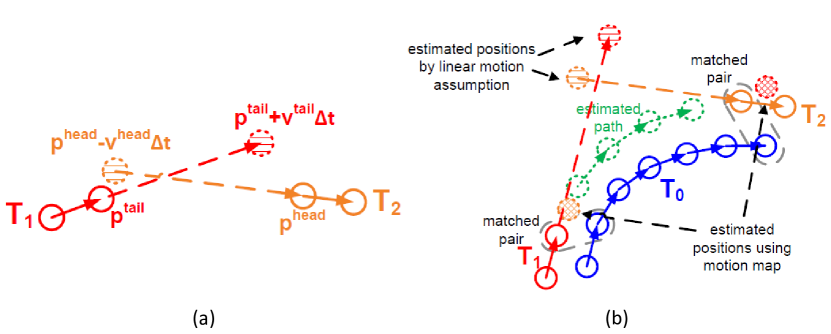
\includegraphics[width=0.95\linewidth]{pictures/motion_linear_nonlinear.png}
    \caption{Comparison of linear motion model (a) with the non-linear motion model (b)}
    \label{fig:motion_linera_non_linear}
\end{figure}

\paragraph{Challenges and Limitations:}
Despite the advancements, SDE methods face significant challenges. Firstly, the separation of detection and embedding tasks leads to high computational complexity. That is since we run detection model, then (instead of getting features directly from detection object detection model) we extract features for each detection using another (reid) model. Offline methods, while accurate, are not applicable for real-time tracking (due to computational complexity and their need for global sequence information. Online methods, although faster struggle with long-term occlusions, similar target interference and irregular motion patterns, as highlighted in the papers \cite{sota-trackets-survey, lit-review}. These methods are highly rely on detector performance; poor detections in complex scenes can propagate errors to the embedding and association stages.


\subsection{Joint Detection and Embedding (JDE) Paradigm}
\label{sec:Joint_detection_embedding}

\paragraph{Overview the JDE paradigm}
The JDE approach training a single neural network to predict both bounding boxes and ReID embeddings \cite{JDE-person-search}. , reducing the computational cost associated with separate models in SDE. According to authors \cite{sota-trackets-survey} JDE paradigm is primarily designed for online tracking.  

\begin{itemize}
\item The \textbf{foundational JDE method}, introduced by Wang et al. (2020) \cite{Toward-RLMOT} integrates Faster R-CNN \cite{fasterRCNN} with an embedding head to simultaneously output detections and appearance features. It achieves a MOTA of 64.4\% on MOT16 with an inference speed of 18.8 FPS. However, its reliance on anchor-based detection limits performance in crowded scenes (due to IoU matching logic). 
\item \textbf{FairMOT} \cite{FairMOT}: Zhang et al. (2021) propose FairMOT, which addresses the trade-off between detection and ReID tasks. It use CenterNet-based anchor-free detector and a parallel ReID branch. FairMOT achieve a MOTA of 73.7\% on MOT16 and 72.3\% on MOT17, with 25.9 FPS. The key advantage is its ability to handle diverse object scales and reducing identity switches (IDSW, 524 on MOT16).
\item \textbf{TransMOT} \cite{TransMOT}: TransMOT introduce transformer architectures to enhance JDE. By integrating spatial-temporal attention mechanisms \cite{Spatial-Temporal-Attention}, TransMOT captures long-range dependencies, improving tracking in occlusion-heavy scenarios. It achieves a MOTA of 76.9\% on MOT17, outperforming FairMOT in complex scenes but with higher computational inference (15.2 FPS).
\item \textbf{CSTrack} \cite{CSTrack}: Liang et al. (2020-2022) introduce a cross-attention mechanism to model interactions between detection and ReID features. This improves feature discriminability, resulting in a MOTA of 74.9\% on MOT17 and 71.8\% on MOT20, with 21.3 FPS. Overall, CSTrack excels in crowded environments, but struggles with irregular motion patterns.
\end{itemize}

\paragraph{Challenges and Limitations:}
Despite its advantages, JDE faces several challenges. Single model for detection and ReID tasks can lead to conflicts, as the two objectives may compete for network capacity, resulting in suboptimal performance for one or both tasks \cite{JDE-person-search}. For example early JDE models \cite{JDE-person-search, Toward-RLMOT} struggled with crowded scenes due to anchor-based detection limitations. FairMOT try to solve that problem using anchor-free detection, however it still faces with long-term occlusions and similar target interference \cite{FairMOT, sota-trackets-survey}. Also in JDE paradigm single model ought to be trained for both detection and ReID, it significantly reduce the avaliable data for training. (Detection model might be trained on Object detection dataset which are larger that MOT datasets, similarly for REiD model). Because of that JDE methods generally lag behind SDE methods like ByteTrack \cite{ByteTrack} in terms of raw MOTA scores (e.g., ByteTrack’s 80.3\% vs. TransMOT’s 76.9\% on MOT17).

\subsection{Tracking by regression (TBR)}
\label{sec:Tracking_by_regression_TBR}

\paragraph{Overview of the TBR Paradigm}
In TBR the focus is shifted from detection-association pipelines to direct trajectory prediction, treating tracking as a regression problem, where models trained to estimate object positions or motion offsets over time \cite{trackformer, MOTR}. By jointly optimizing these components (detection, motion prediction, and association), TBR approach reduce computational costs while archiving good accuracy, particularly in occlusion-heavy and crowded scenes.

\begin{figure}[h]
    \centering
    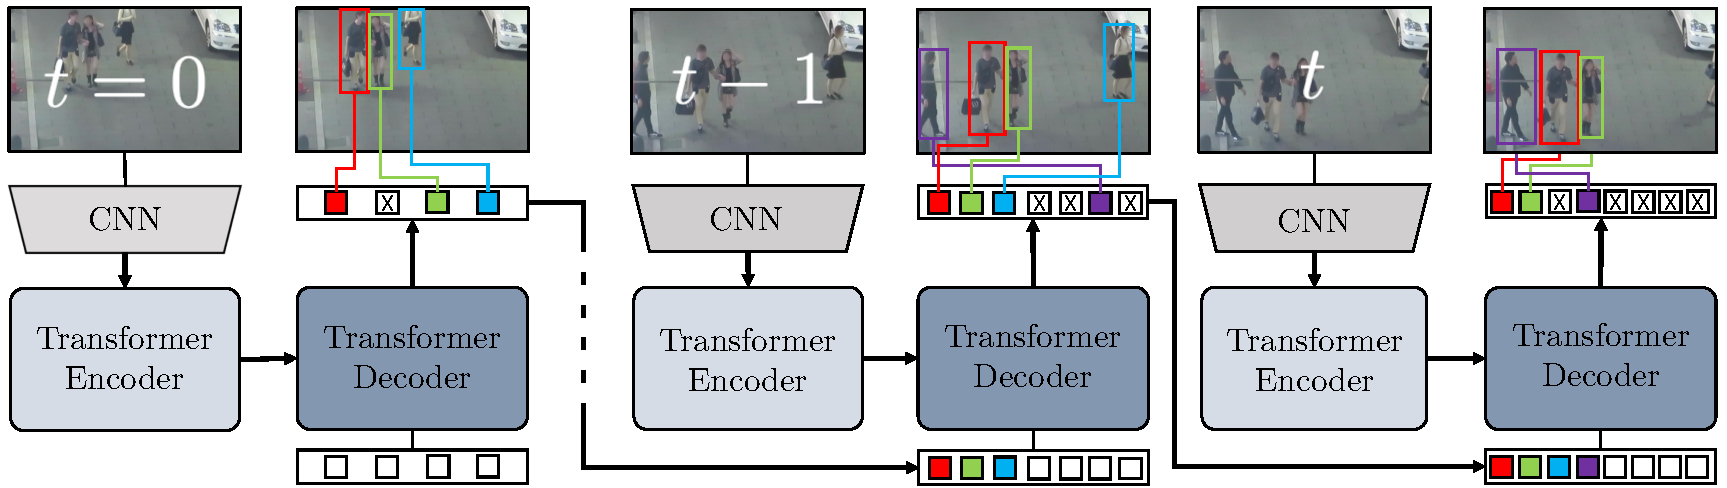
\includegraphics[width=0.95\linewidth]{pictures/trackFormer.pdf}
    \caption{\textbf{TrackFormer} treats MOT as a set prediction problem performing joint detection and \textbf{tracking-by-attention}. The architecture consists of a CNN for image feature extraction, a Transformer encoder for image feature encoding and a Transformer decoder which applies self- and encoder-decoder attention to produce output embeddings with bounding box and class information. At frame $t = 0$, the decoder transforms $N_\text{object}$ object queries (white) to output embeddings either initializing new autoregressive \textbf{track queries} or predicting the background class (crossed). On subsequent frames, the decoder processes the joint set of $N_\text{object} + N_\text{track}$ queries to follow or remove (blue) existing tracks as well as initialize new tracks (purple).}
    \label{fig:TrackFormer}
\end{figure}

\paragraph{Key Papers in TBR Development}
\begin{itemize}

    \item \textbf{FAMNet} \cite{FAMNet} pioneers end-to-end joint optimization of feature extraction, affinity estimation, and multi-dimensional assignment. In the paper all layers of network are designed differentiable, thus can be optimized jointly to learn the discriminative features and higher-order affinity model, which is supervised by the loss directly from the assignment ground truth. Authors also integrate Single object tracking (SOT) technique to recover false negatives and suppress detector noise.

    \item \textbf{Tracktor++} \cite{Tracktorpp} repurposes an object detector’s bounding box regression to predict object positions across frames (In particular, authors perform no training or optimization on tracking data). In additions authors uses camera motion compenstation and simple reid model. However in their original paper authors state it as "as a new tracking paradigm" only, because it tackles with complex scenarios. But the work is still worth-mentioned because of the novelty of their approach. \textit{Note: Tracktor++ is in fact a Hybrid tracker, because it employ separate reid model as additional module.}

    \item \textbf{TrackFormer}\cite{trackformer}: Meinhardt et al. (2022) propose TrackFormer, a transformer-based TBR method that treats tracking as a set prediction problem. In this paper authors employ an encoder-decoder architecture to predict bounding boxes and track identities Fig. ~\ref{fig:TrackFormer}. This approach achives MOTA of 62.1\% on MOT17 with 25.9 FPS. Main strength lies in modeling long-range temporal dependencies, however such approach struggles in crowded scenes due to limited ReID integration.

    \item \textbf{CTracker} \cite{CTracker}: introduces a chained structure that links paired bounding boxes across adjacent frames via attentive regression (combining object- and identity-attention). This end-to-end approach achives MOTA of 66.6\% without extra training data, but its frame-by-frame chaining struggles with long-term occlusions. \textit{Note: some authors categorize it as TBD model, some authors \cite{sota-trackets-survey} as TBR.}.

    \item \textbf{TubeTK} \cite{TubeTK}. In this work authors proposes bounding tubes—temporal sequences of boxes—to capture spatio-temporal consistency in short clips. This model outperforms TBD methods on occlusion handling but requires clip-based processing, limiting real-time applicability.

    \item \textbf{RetinaTrack} \cite{RetinaTrack}. RetinaTrack unifies detection and tracking using instance-level embeddings. It outperforms two-stage trackers on the Waymo Open Dataset with lower computational cost, though its performance depends heavily on (RetinaNET's) embedding quality. 

    \item \textbf{TADAM} \cite{TADAM}. Authors unifies position prediction and embedding association through \textbf{temporal-aware attention} and distractor suppression. Using memory aggregation module TADAM enhances identity awareness (reducing IDSW). However the inference itself is computationally costly, trading accuracy for speed.

    \item \textbf{CenterTrack} \cite{CenterTrack}. In this paper authors use pairs of frames and prior detections. It achieves 67.8\% MOTA on MOT17 at 22 FPS and can be extended to 3D tracking with minimal modifications. However association in this work relies heavily on motion cues, struggling with appearance-based distractors.

    \item \textbf{CorrTracker} \cite{CorrTracker}. Authors addresses CNN's limitations in capturing long-range spatial and temporal dependencies. Unlike TBD, CorrTracker introduces learnable correlation operations to model topological relationships between objects and their surroundings (Fig. ~\ref{fig:Corrtrack}). \textbf{Local Correlation Module} solve CNN's limited receptive field using \textbf{Dense Correspondence Matching}. For each spatial location (e.g., an object bounding box), CorrTracker computes correlation value with its surrounding context via self-supervised learning. \textbf{Temporal Correlation Learning} (Motion Modeling) archive better performance on irregular motion patterns, changing simple motion models (e.g., Kalman filters) or short-term feature matching. CorrTracker’s correlation mechanism has influenced later works, such as: \textbf{TransTrack} (uses attention for cross-frame correlation) and \textbf{OC-SORT} (integrates motion correlation with observation-centric recovery) \cite{TransTrack, TransMOT, os-sort}.
\end{itemize}

\begin{figure}[h]
    \centering
    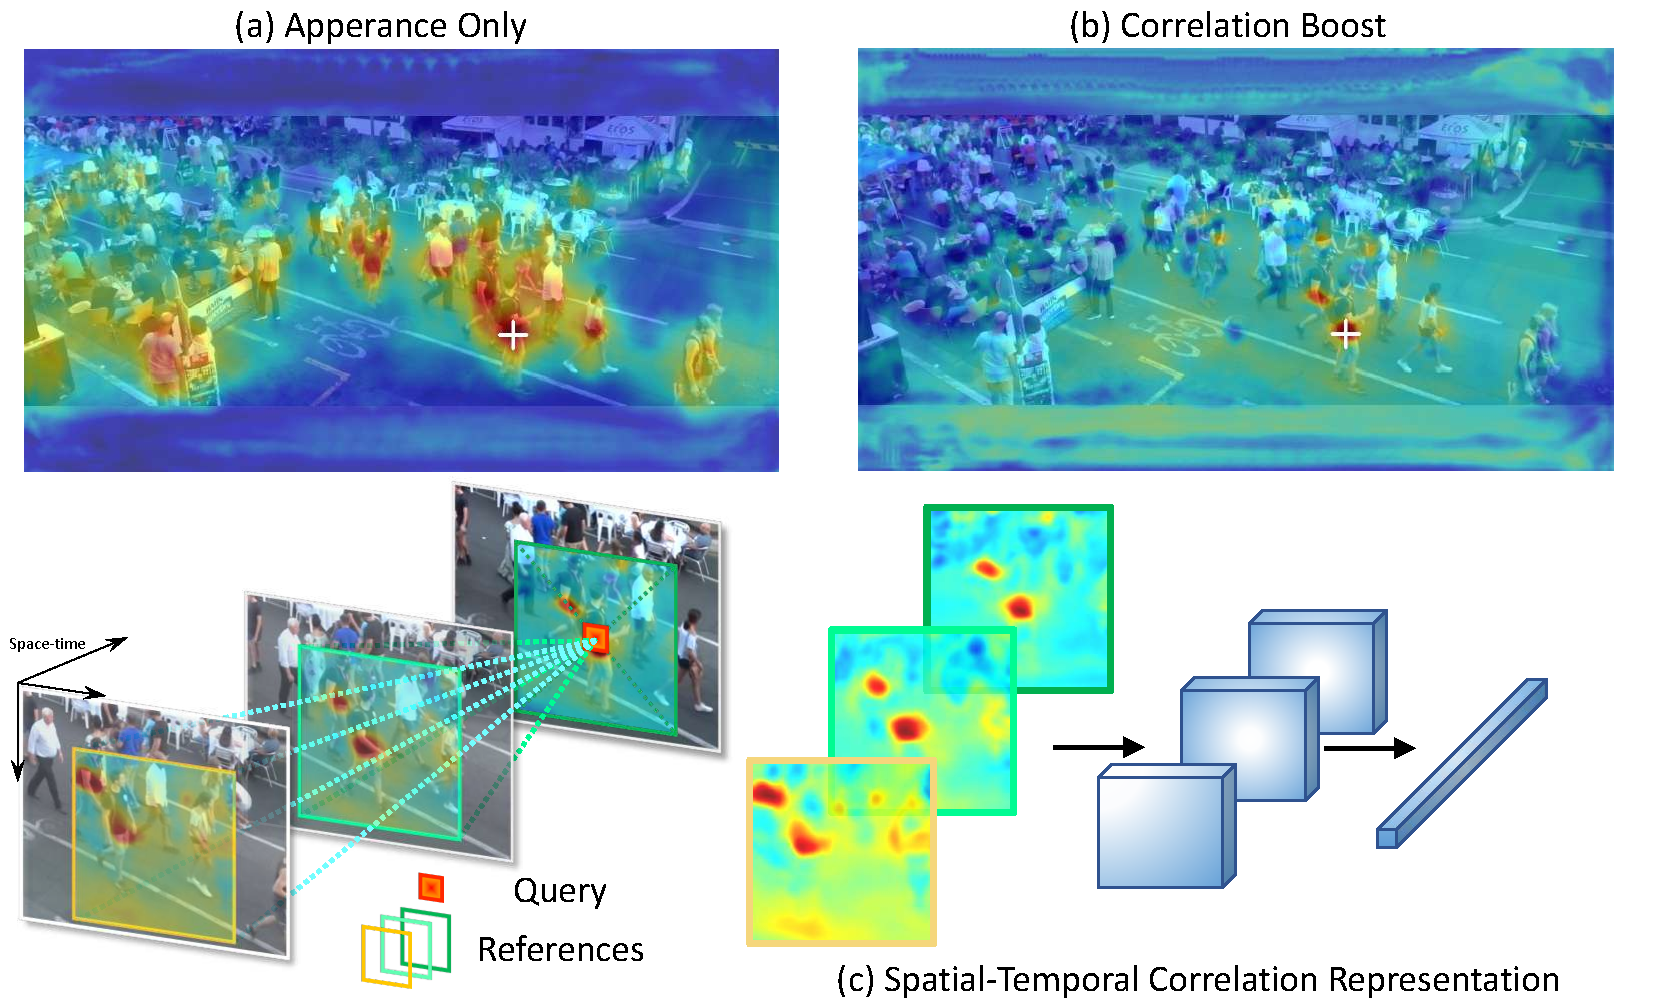
\includegraphics[width=0.8\linewidth]{pictures/CorrTrack.pdf}
    \caption{Comparison of linear motion model (a) with the non-linear motion model (b)}
    \label{fig:Corrtrack}
\end{figure}


\subsection{Tracking by attention}
\label{sec:Tracking_by_attention_TBA}

\paragraph{Overview}
The transformer architecture, originally designed for natural language processing (NLP) \cite{early_attention, attention-is-all-you-need} \textit{(I can't resist quoting this paper)} later was adopted in computer vision by enabling long-range dependencies and high-order spatial interactions through self-attention. In MOT, vision transformers (ViTs) Fig. \ref{fig:vision_trasformer} \textit{(For me good explanation was found in \cite{ViT-survey, ViT-how-works})} excel at modeling complex object relationships across frames, but face challenges in computational efficiency and handling new object appearances. \textit{Note: in fact I it's not a separate category of MOT trackers, because attention based models are also found among TBR and JDE paradigms}

\paragraph{Key Papers in TBA Development}
\emph{}


\begin{figure}[h]
    \centering
    \begin{minipage}{0.3\textwidth}
        \centering
        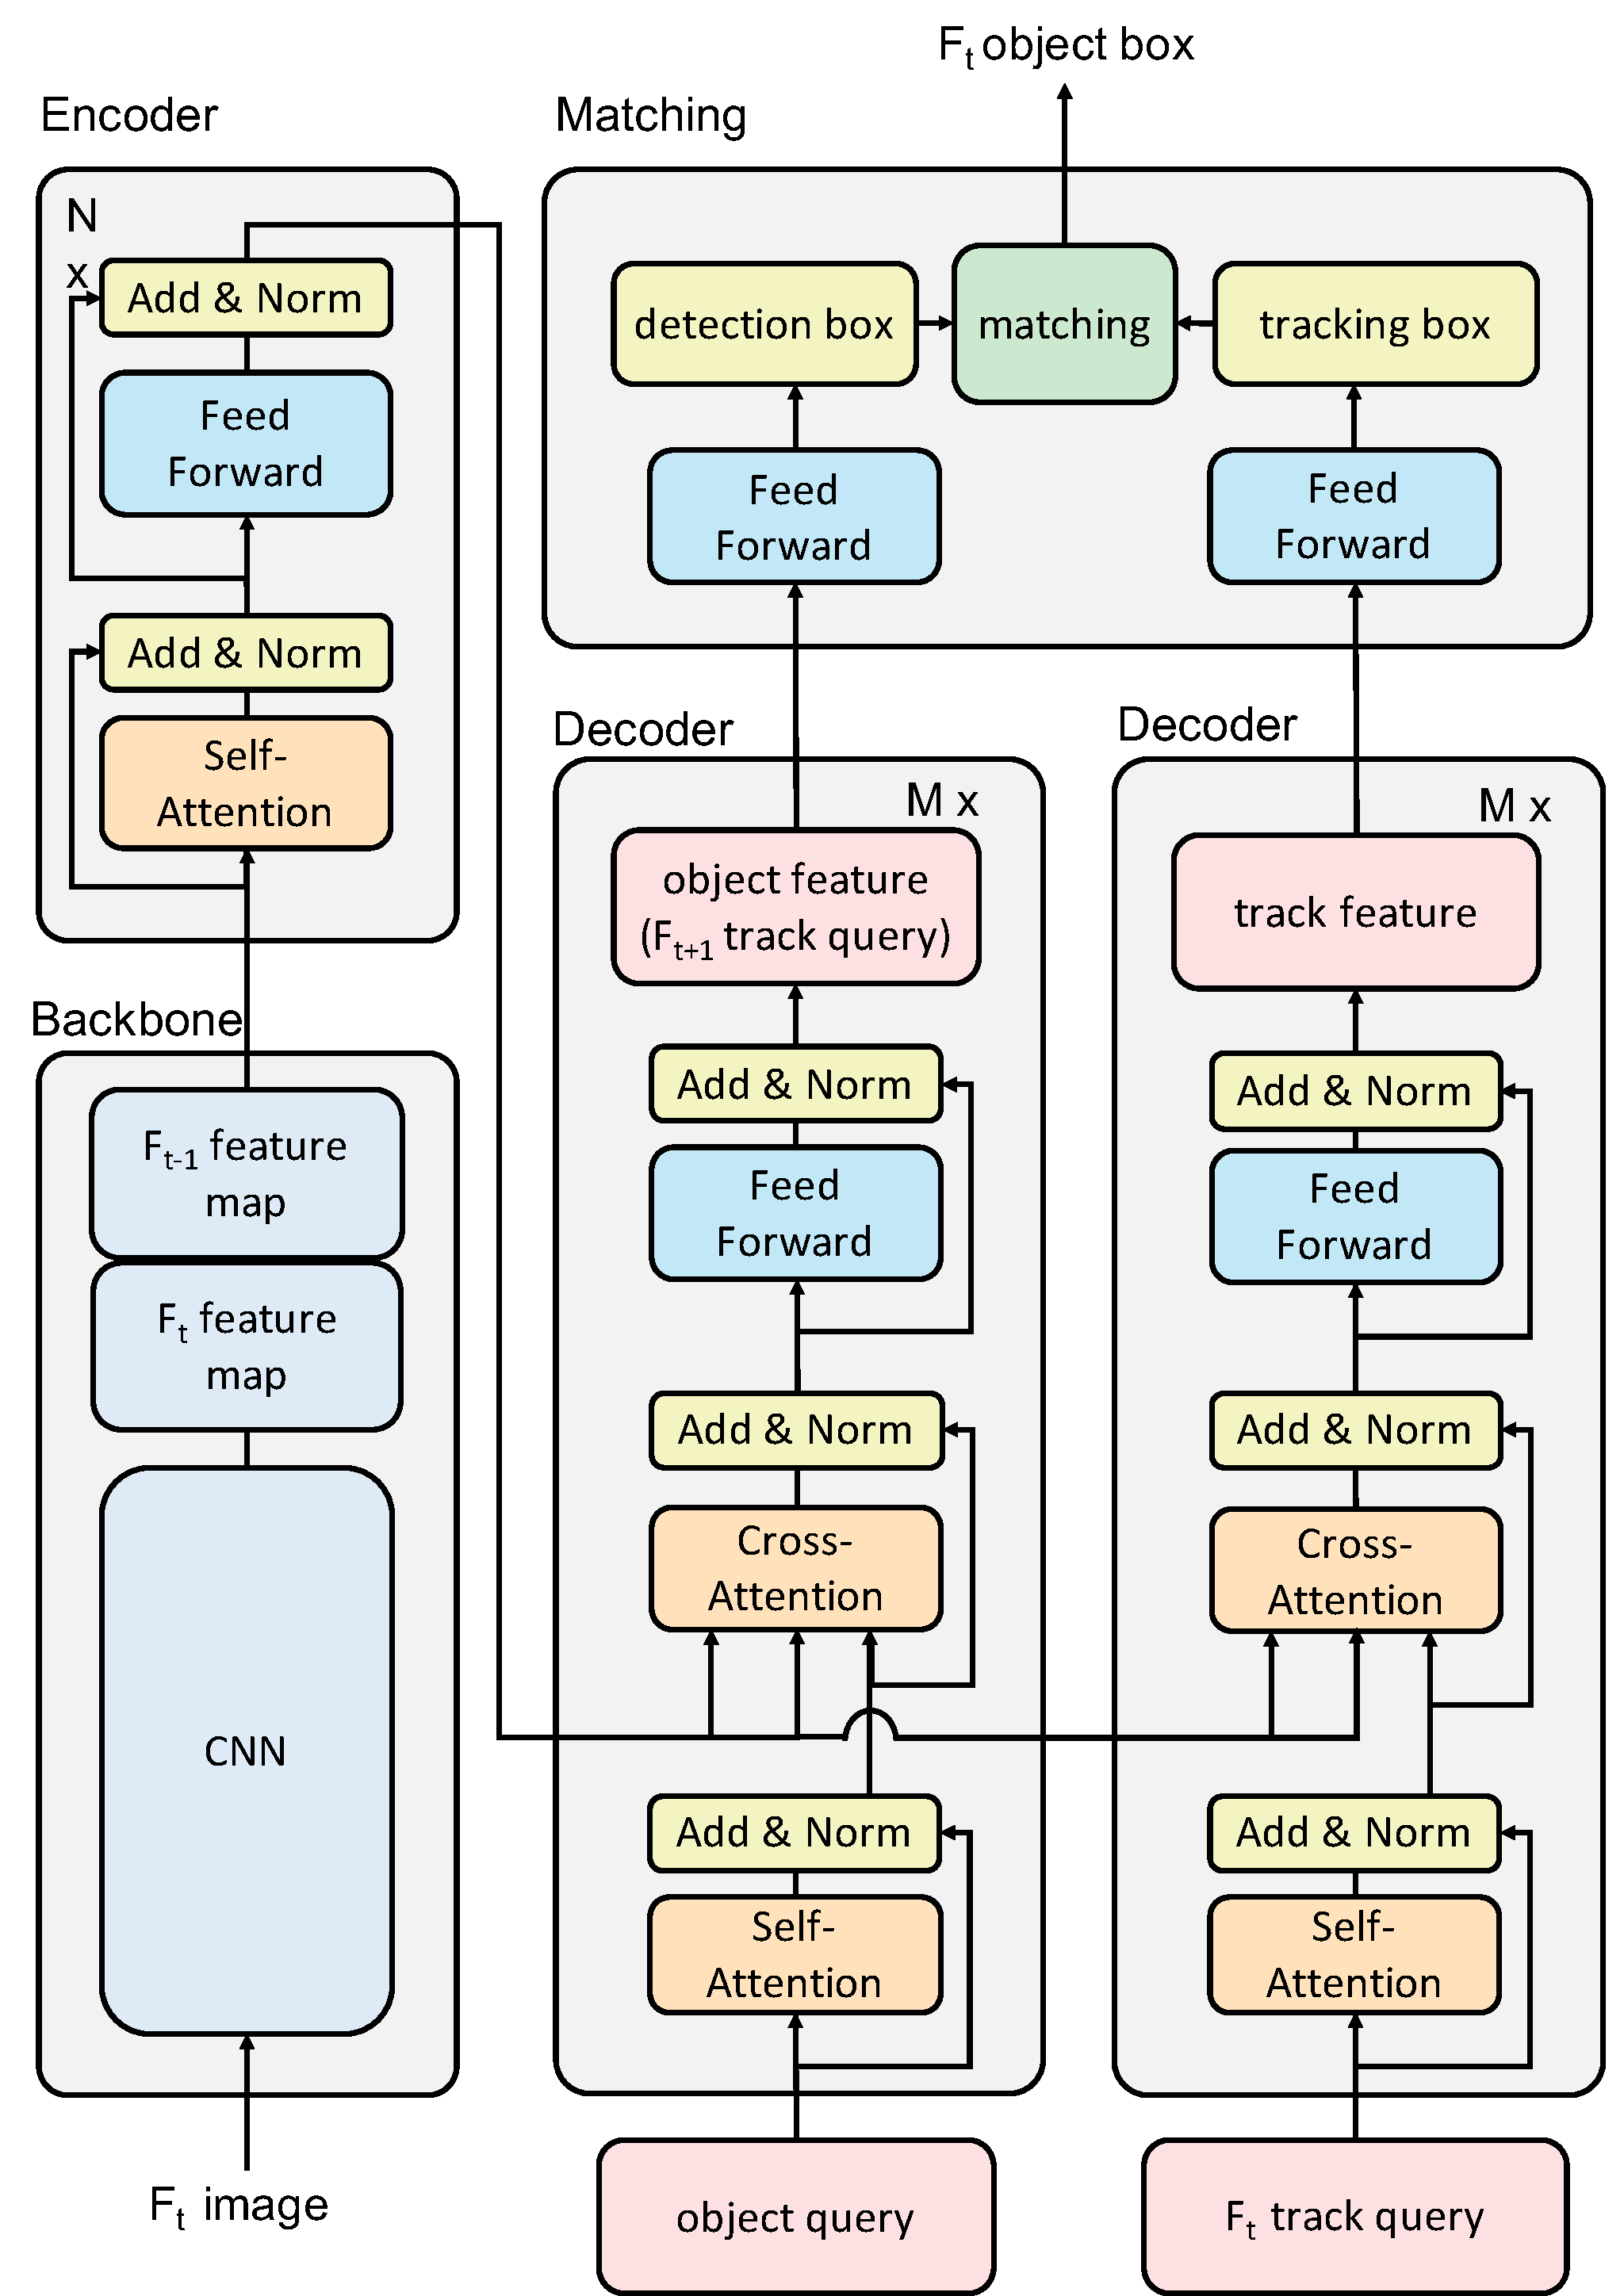
\includegraphics[width=\linewidth]{pictures/transTrack_model.pdf}
        \caption{TransTrack model architecture}
        \label{fig:Transtrack_model}
    \end{minipage}
    \hfill
    \begin{minipage}{0.6\textwidth}
        \centering
        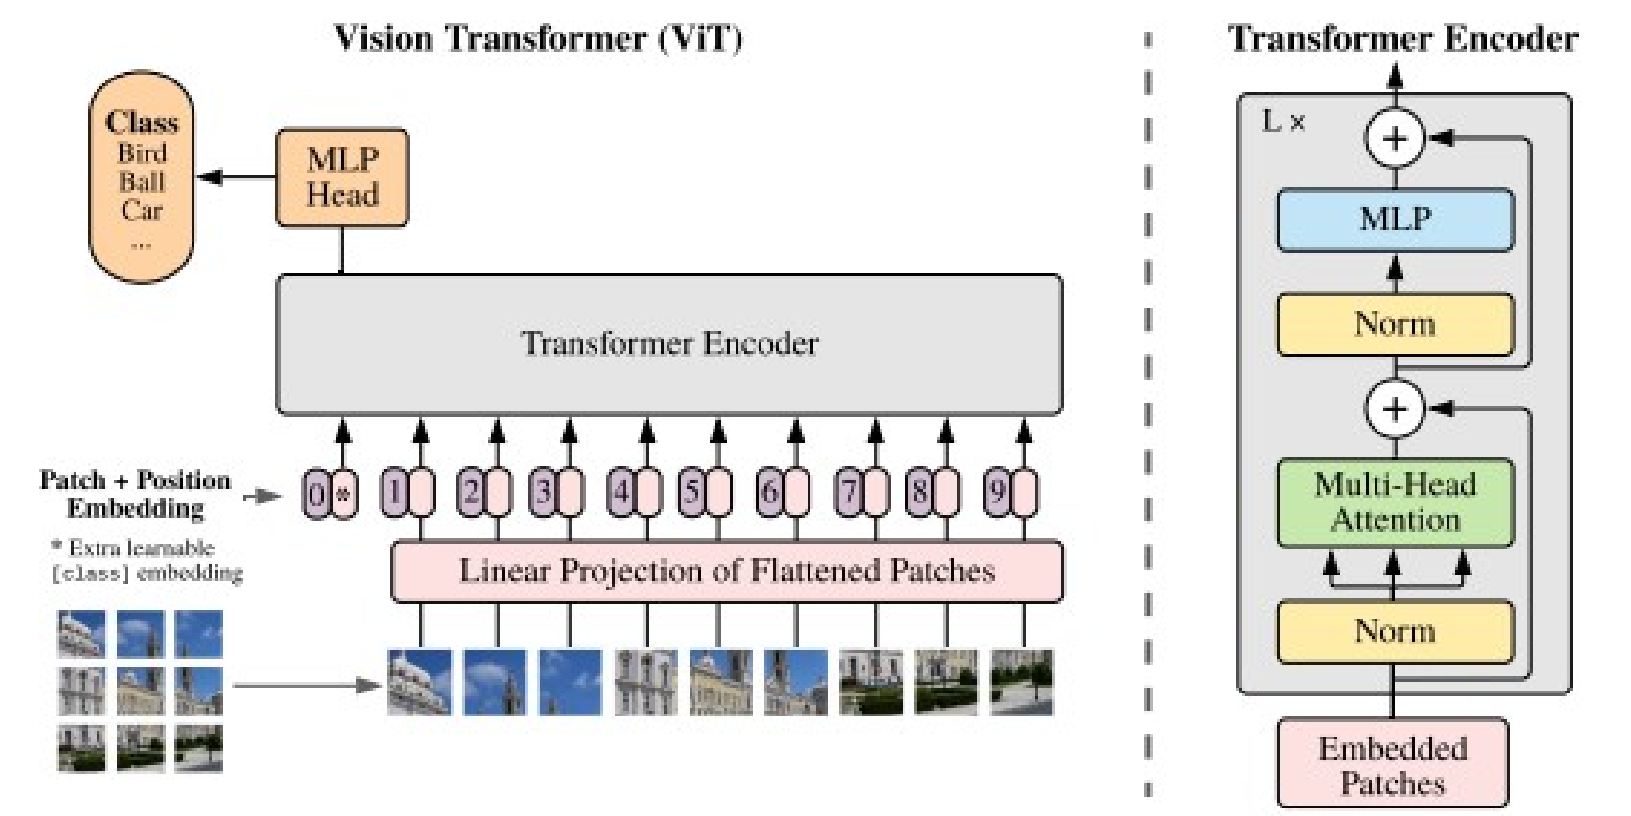
\includegraphics[width=\linewidth]{pictures/VisionTransformer.pdf}
        \caption{Vision Transformer illustrative example}
        \label{fig:vision_trasformer}
    \end{minipage}
\end{figure}

\textbf{TransTrack}, Introduced by Sun et al. in 2020, was pioneered in transformer-based MOT. It simplifies the tracking pipeline by integrating joint detection and tracking in a single shot. The system processes consecutive frames through an encoder-decoder architecture, where a shared encoder generates feature maps, and dual decoders produce detection and tracking boxes Fig. ~\ref{fig:Transtrack_model}. These are matched using IoU-based Hungarian algorithm to form ordered object sets, eliminating the need for non-maximum suppression. However TransTrack struggles with crowded scenes and small objects due to limited ReID integration. Its computational complexity, lags behind faster methods like FairMOT \cite{FairMOT}. 

TrackFormer \cite{trackformer} employs a DETR detector and seamlessly forms target trajectories across multiple video frames in an autoregressive manner. By constructing a spatial graph transformer encoder, a temporal transformer encoder and a spatial graph transformer decoder, it organizes the tracking trajectories of each object into a set of weighted sparse graphs \cite{k-shortest-paths-for-mot, GMCP-tracker, tensor-based-high-order-graph-matching}, successfully modeling spatial and temporal interactions between potentially multiple objects. \textbf{TrackFormer}\cite{trackformer} and \textbf{MOTR} \cite{MOTR} also corresponds to TBA (it was mentioned above); 

\subsection{Comparison of Multiple Object Tracking (MOT) Paradigms}

\begin{table}[H]
\centering
\caption{Comparison of MOT Paradigms}
\begin{tabular}{|>{\raggedright\arraybackslash}m{2cm}|>{\raggedright\arraybackslash}m{4cm}|>{\raggedright\arraybackslash}m{3.5cm}|>{\raggedright\arraybackslash}m{4.5cm}|>{\raggedright\arraybackslash}m{3.5cm}|}
\hline
\textbf{Paradigm} & \textbf{Key Characteristics} & \textbf{Strengths} & \textbf{Challenges} & \textbf{Performance Examples} \\
\hline
\textbf{SDE} & Separates detection and ReID tasks; offline uses batch processing, online uses current/past frames. & High accuracy in occlusion-heavy scenes (offline); real-time capability (online). & High computational complexity; offline impractical for real-time; online struggles with long-term occlusions, similar targets. & DeepSORT: 61.4\% MOTA (MOT16), ByteTrack: 80.3\% MOTA (MOT17). \\
\hline
\textbf{JDE} & Single model for detection and ReID; primarily online tracking. & Reduced computational cost; handles diverse object scales (e.g., FairMOT). & Conflicts between detection/ReID tasks; limited training data; struggles with crowded scenes, long-term occlusions. & FairMOT: 73.7\% MOTA (MOT16), TransMOT: 76.9\% MOTA (MOT17). \\
\hline
\textbf{TBR} & Direct trajectory prediction via regression; joint optimization of detection, motion, association. & Low computational cost; effective in occlusion-heavy/crowded scenes; models long-range dependencies. & Limited ReID integration; struggles with long-term occlusions or appearance-based distractors. & TrackFormer: 62.1\% MOTA (MOT17), CenterTrack: 67.8\% MOTA (MOT17). \\
\hline
\textbf{TBA} & Transformer-based for long-range dependencies; overlaps with TBR/JDE. & Excels in complex object relationships; simplifies pipeline (e.g., TransTrack). & High computational complexity; struggles with crowded scenes, small objects, new appearances. & TransTrack: Limited ReID integration, TrackFormer: 62.1\% MOTA (MOT17). \\
\hline
\label{MOT_paradigms_table}
\end{tabular}
\end{table}

\section{ReID Approaches}

\begin{figure}[h]
    \centering
    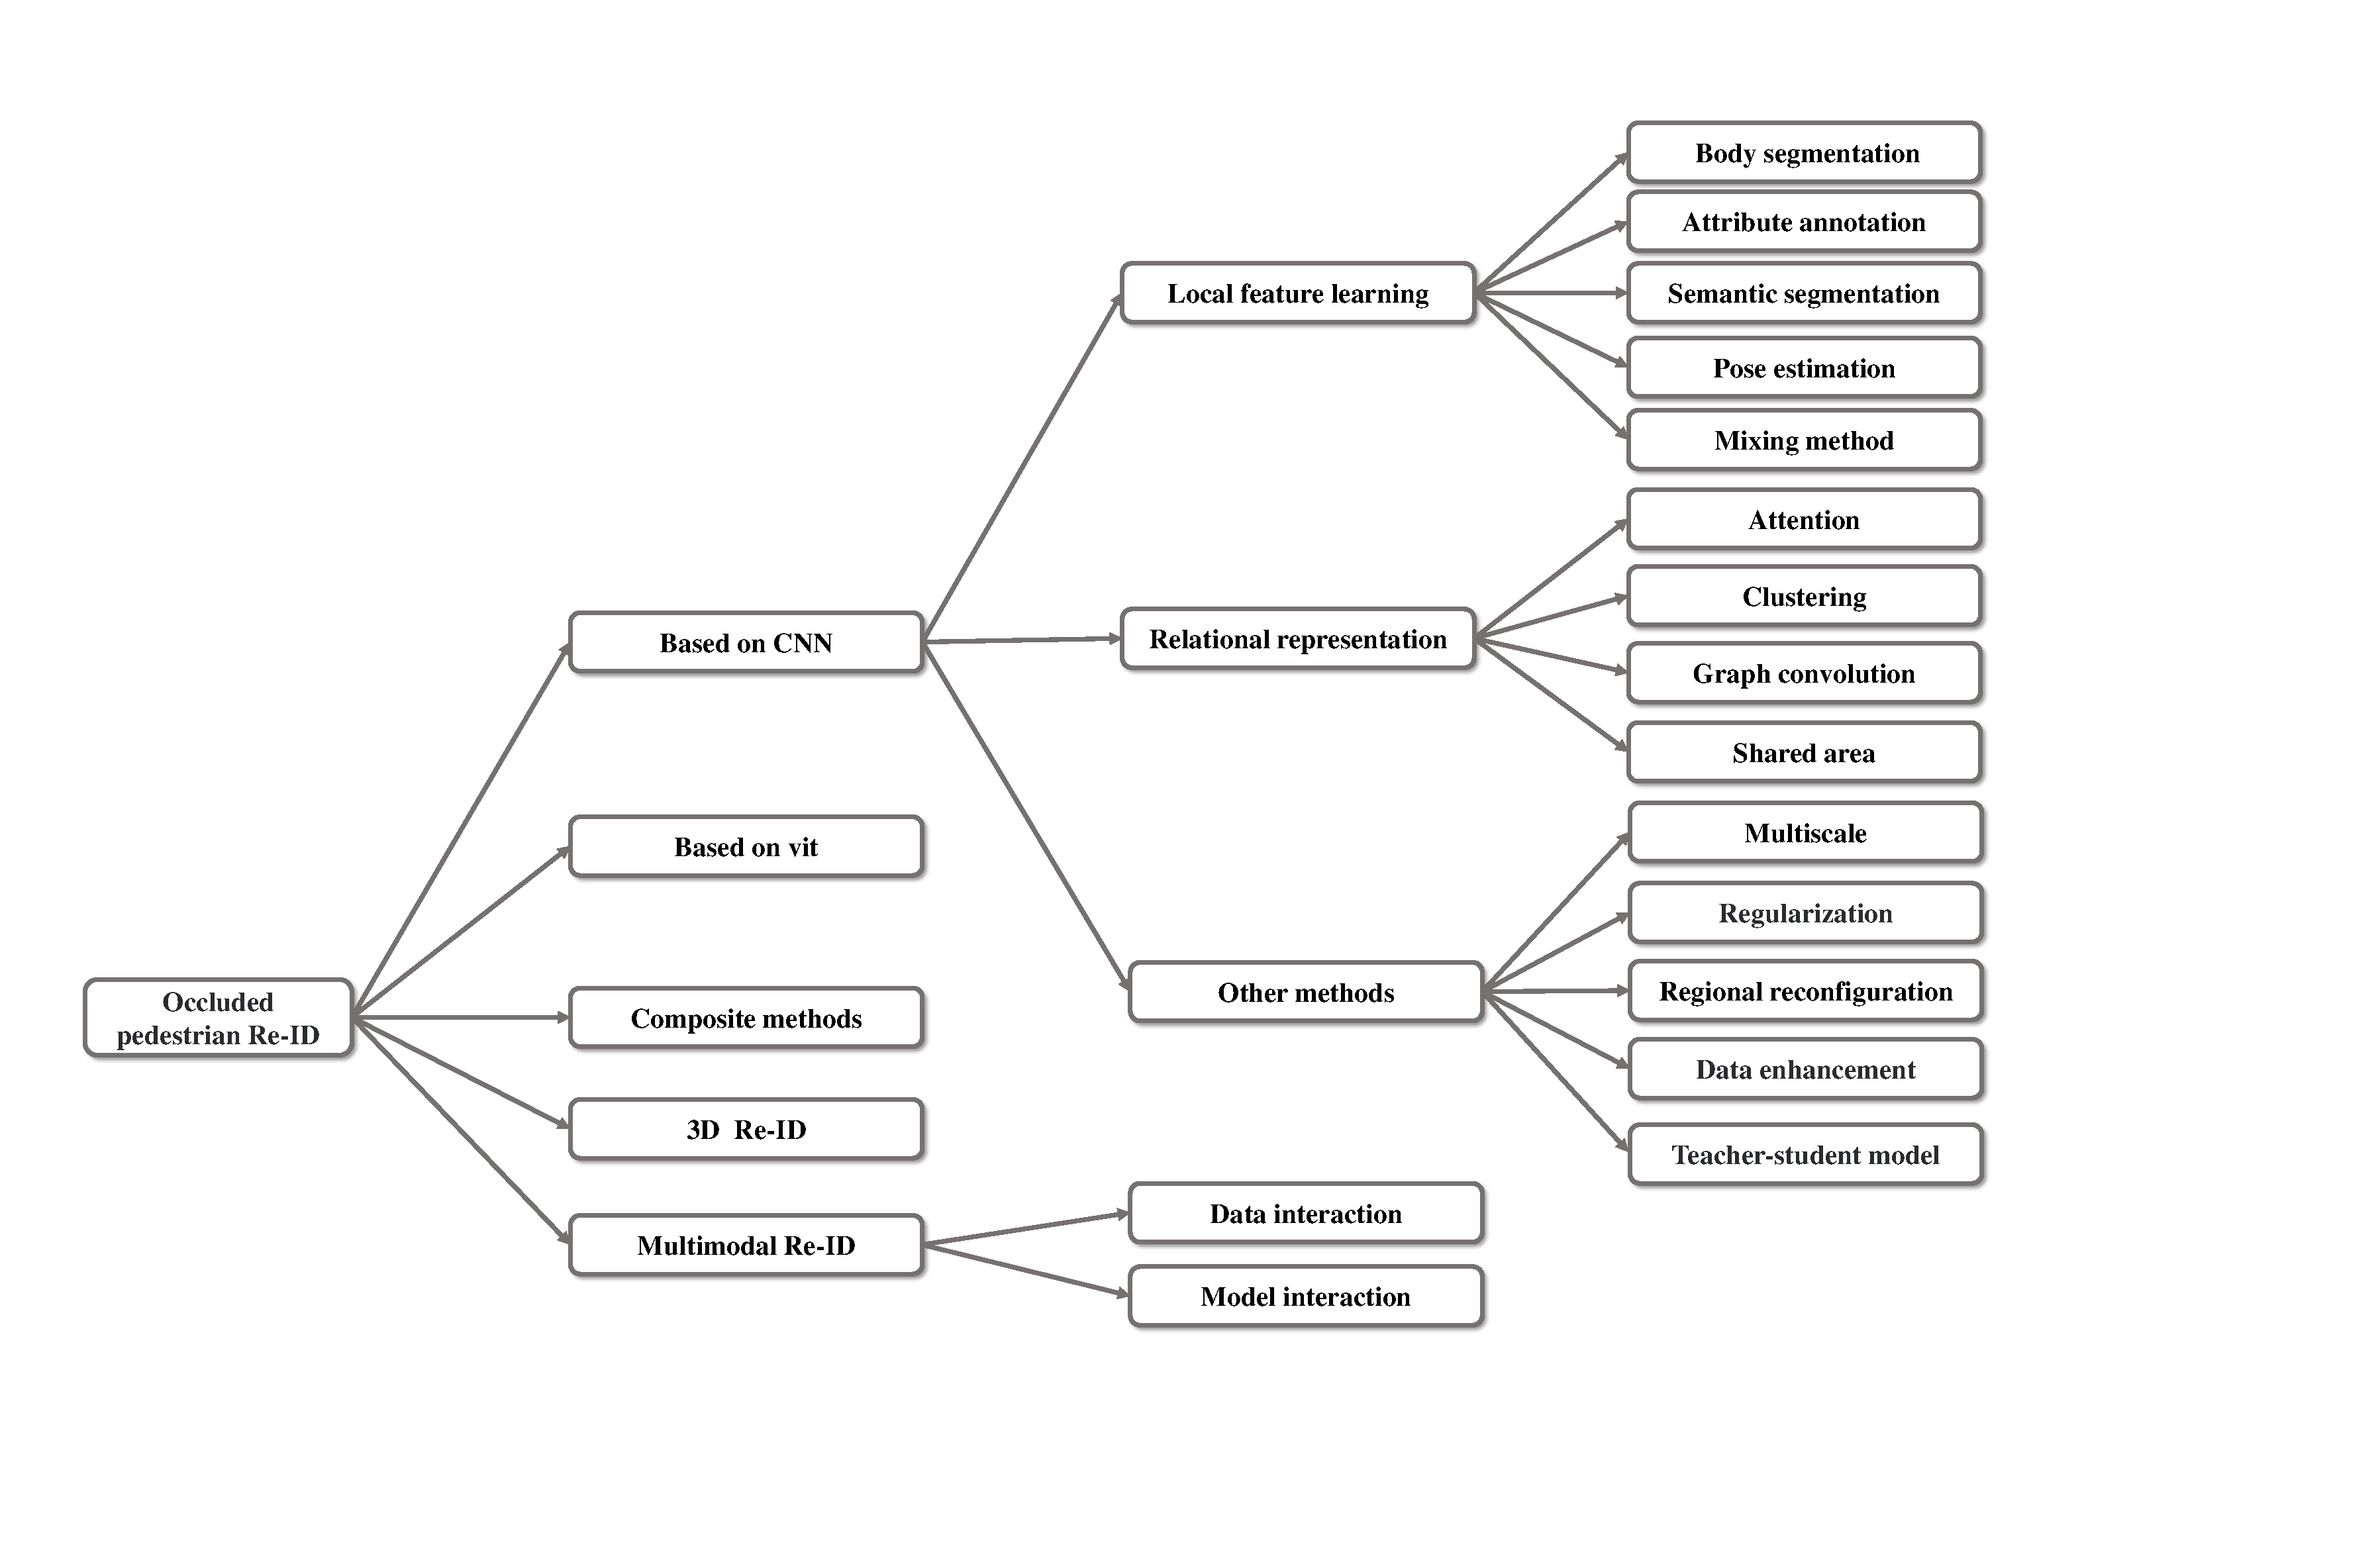
\includegraphics[width=0.8\linewidth]{pictures/reid_models_cat.pdf}
    \caption{Overall structure of ReID approaches}
    \label{fig:reid_models_cat}
\end{figure}

\paragraph{Intro} Person re-identification (Re-ID) is a critical component of solving MOT problem, aiming to match identities despite challenges like occlusion, noise, and misalignment. In this segment I focus on deep learning-based Re-ID models. Authors of this magnificent survey \cite{reid_survey} categorize the approaches into five main paradigms Fig.~\ref{fig:reid_models_cat}:
\begin{itemize}
    \item \textbf{CNN-based Methods} - early method, which extracts local and relational features, 
    \item \textbf{Transformer-based Methods} - utilize Vision Transformers (ViTs) for capturing long-range dependencies and detailed contextual information. 
    \item \textbf{Hybrid Structure-based Methods} - combine CNNs and transformers or other architectures.
    \item \textbf{3D Person Re-ID Methods} - work with three-dimensional data (e.g., point clouds) to provide spatial context
    \item \textbf{Multimodal Person Re-ID Methods} - employ multiple data modalities (e.g. RGB, infrared, depth information, etc).
\end{itemize}

\subsection{CNN-based Methods}

CNN models by design excel at extracting local features, making them suitable for occlusion handling by focusing on visible regions or modeling relationships between features. This category is subdivided firther into \textbf{Local Feature Learning}, \textbf{Relational Representation}, and \textbf{Other Methods.}

\paragraph{Local Feature Learning} - Focuses on extracting and using local features.
In this work \cite{DPPR} (deep partial person re-identification (\textbf{DPPR})), authors use an attention-based matching mechanism to prioritize features from body parts. The attention model selects a subset of CNN feature vectors. 
In this work \cite{SPReID} (Semantic Parsing for Person Re-identification 2018), authors employ a semantic parsing model for separating body regions (generating probability maps). This approach allows to explicitly separate body parts (candidates) for matching problem. In HOReID (Hight order topology 2020) the authors employ pose estimation, forming a topological graph to suppress noise Fig.~\ref{fig:horeid}. HOReID creates a learnable Pose-guided relational matrix. Combining pose estimation with graph-based noise suppression 
archives significantly improves previous results. 
A further improvement was proposed in \textbf{GASM} (2020) \cite{GASM} by semantic segmentation and pose estimation to separate pedestrians from backgrounds. Its strength lies in saliency-aware feature extraction through joint semantic and pose guidance. \textbf{CBDB-Net} (2021) \cite{CBDB-Net} proposed removing some parts of feature maps, simulating real-world incomplete data to train more resilient pedestrian representations.

\begin{figure}[h]
    \centering
    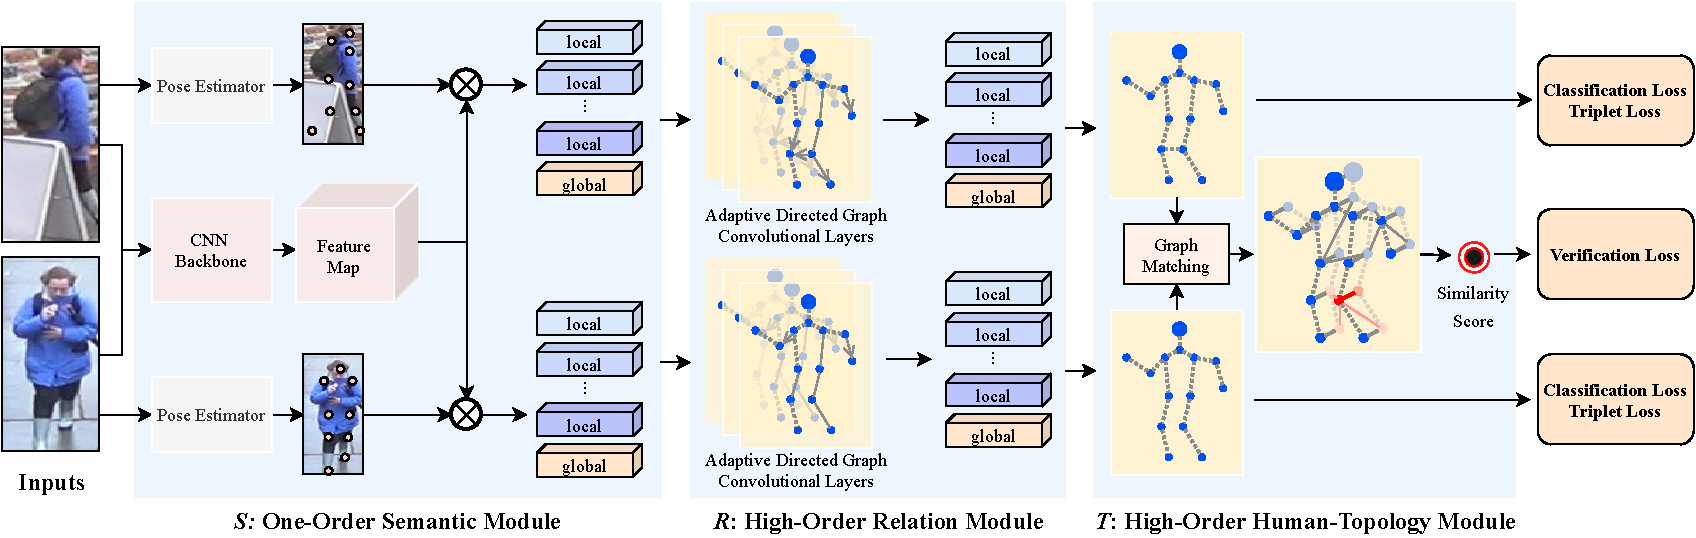
\includegraphics[width=0.9\linewidth]{pictures/HOReid.pdf}
    \label{fig:horeid}
\end{figure}

\paragraph{Relational Representation} - Focuses on learning relationships between features.
In \textbf{AACN} \cite{AACN} proposes using pose-derived attention maps with visibility scores. The authors of this paper focus on visibility-aware attention system for matching unoccluded pedestrian features. In \textbf{VPM} \cite{VPM} authors employ self-supervised model for localization of the visibility of shared regions. Also it uses weighted feature extraction.  In \textbf{ISP} \cite{ISP} authors develops a technique that clusters pixels into pseudo-labels to distinguish person from background in a self-supervised way. (unlike it was done in \cite{GASM}). That paper make a significant step forward in occlusion management, by designing automatic denoising method. 

\paragraph{Other methods}: \textbf{RFCNet} \cite{RFCNet} suggests an encoder-decoder system to restore occluded features using spatial context from non-occluded areas. \textbf{IGOAS} \cite{IGOAS} offers a progressive occlusion augmentation strategy in training section. Such gradual occlusion training approach has proven effective.

\subsection{Transformer-based Methods} 

\textbf{TransReID} \cite{TransReID} First to apply ViT to Re-ID using multi-head self-attention to focus on body parts without downsampling loss. Unlike the predecessors, TransReID excels in preserving details for occlusion scenarios. Later, \textbf{PFD} (Pose-guided Feature Disentangling) \cite{PFD} proposes a transformer encoder with pose-guided feature aggregation, which allows to focus on visiable parts. Such combination of of pose and transformer technology improves discriminative feature separation. \textbf{FED} (Feature Erasing and Diffusion Network) \cite{FED} addresses non-target pedestrian occlusion with feature erasure and diffusion. This non-target feature removing (via score diffusion) imroves robutness by reducing non-target features impact. 

\subsection{Hybrid Structure-based Methods}

Recent advancements have introduced sophisticated models like the Pose-guided Inter- and Intra-part Relational Transformer (\textbf{Pirt}) and the Fine-Grained Multi-Feature Fusion Network (\textbf{FGMFN}). 

\begin{figure}[h]
    \centering
    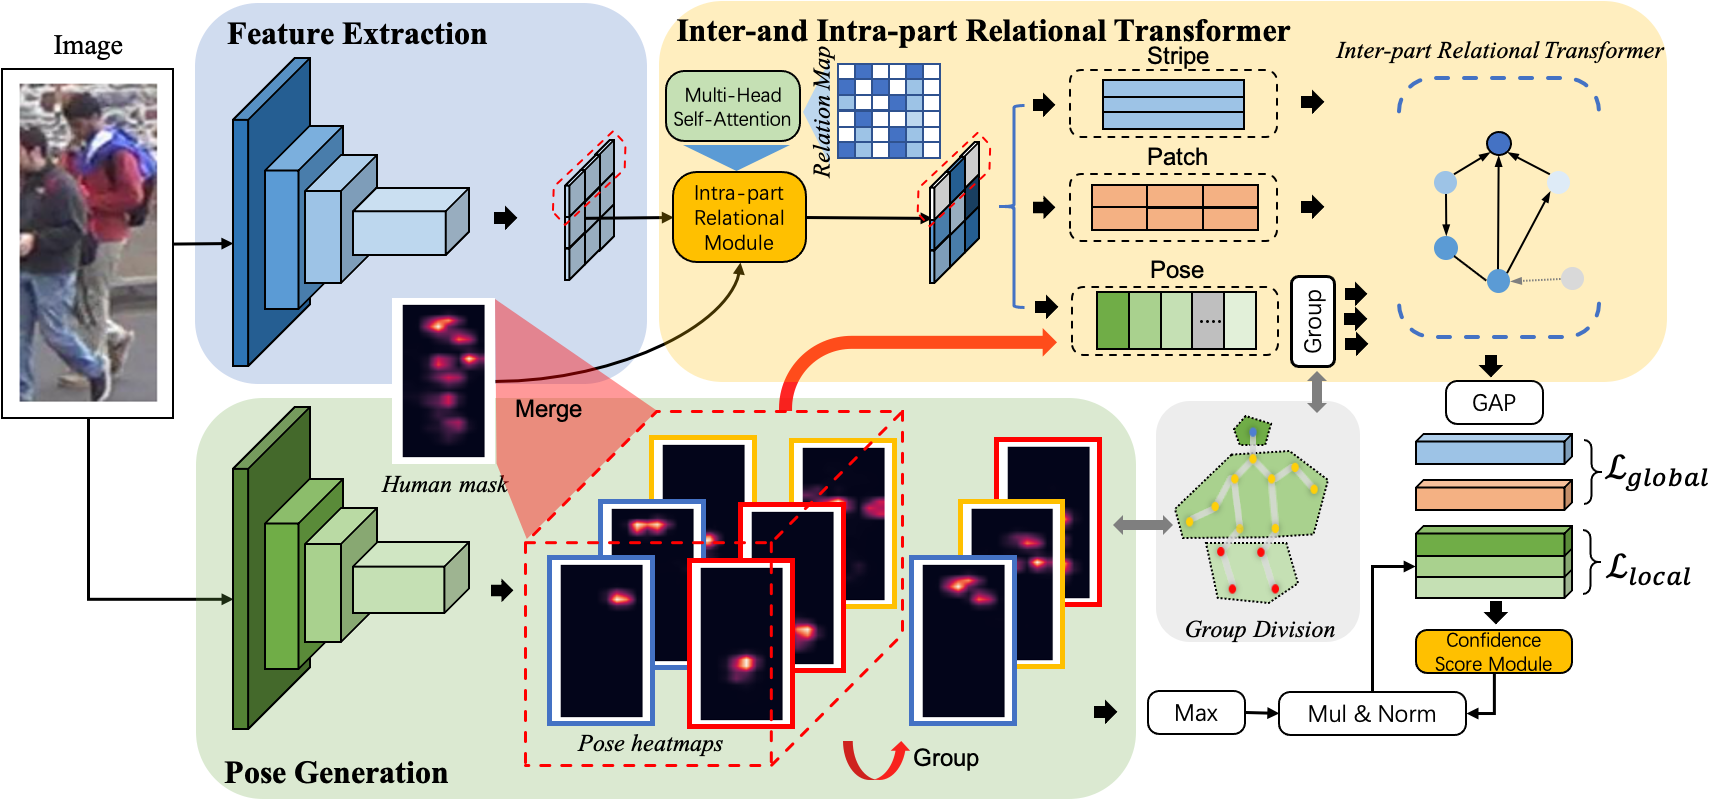
\includegraphics[width=0.9\linewidth]{pictures/pirt_pipeline.png}
    \caption{Pirt overall architecture}
    \label{fig:pirt_pipeline}
\end{figure}

 The \textbf{Pirt} \cite{Pirt} model use pose estimation and expand keypoint regions into larger masks and grouping them. As shown at the Fig.~\ref{fig:pirt_pipeline} Pirt employs a dual relational approach: an intra-part module extracting local relations using mask-guided features. The inter-part relational transformer captures long-range correlations between different part nodes, treating each part (features of this body part) as a graph node within the transformer architecture. Also Pirt utilizes striped slices (as in \cite{IGOAS}), patched grids and pose-keypoint regions.  For final matching it  ntegrates global features with these part-based local features for improving robutness.

 The \textbf{FGMFN} model \cite{FGMFN}, conversely, operates as a dual-branch network designed to extract discriminative features without using an external pose estimation models Fig. ~\ref{fig:FGMFN_pipe}. In global feature branch it employes a chinking strategy, diviging the feature map into original, tow-division and three-division segments to capture multi-granularity features.  In partial feature branch it utilizes a Spatial Transformer Network \cite{Spatial-Temporal-Attention} to automatically localize the pedestrian's upper body. Then the feature map of this upper body region is horizontally segmented into three part, and Relation-aware Attention Module (RAM) applied to each part to extract fine-grained information and further improve discriminative details. Finally, features from both branches are fused archiving robust feature representation for further matching. 

 \begin{figure}[h]
    \centering
    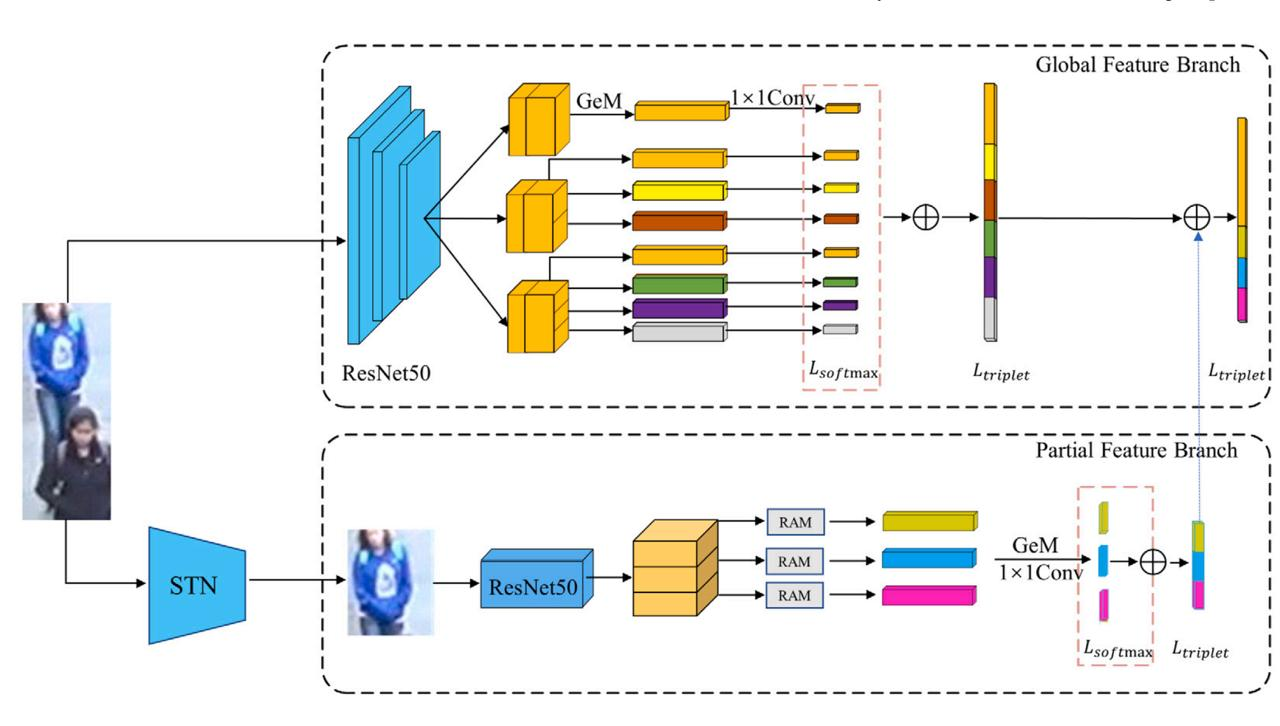
\includegraphics[width=0.8\linewidth]{pictures/FGMFN_pipe.jpeg}
    \caption{\textbf{FGMFN} architecture. STN is the Spatial Transformer Network module, RAM is the Relation-aware Attention Module, GeM stands for Generalized-mean pooling, and $\bigoplus$ denotes feature concatenation operation}
    \label{fig:FGMFN_pipe}
\end{figure}

\subsection{3D Person Re-ID Methods}
Key component of 3D Person Re-ID is Three-dimensional human pose estimation. It involves determining the 3D locations of articulated body joints from images or videos. It helps Re-ID because it gives more detailed spatial information than 2D methods, making it easier to tell people apart, especially when they are partly hidden or seen from different angles. Human body structure in this context is often represented using \textbf{skeleton-based models}, which depict the body as a tree structure of keypoints connected by edges, or more complex parametric models like the \textbf{Skinned Multi-Person Linear model (SMPL).} \cite{SMPL}. The SMPL model represents the human skin as a triangulated mesh with thousands of vertices, parameterized by shape and pose, allowing for detailed 3D body joint estimation. Another notable representation was proposed in DensePose \cite{DensePose}. The authors established dense correspondences between image pixels and a surface-based 3D model of the human body. Fig.~\ref{fig:DensePose}. In fact, 3D pose estimation methods typically involve either \textbf{directly predicting 3D coordinates} from images or \textbf{"lifting" 2D pose estimations} into 3D space.

 \begin{figure}[h]
    \centering
    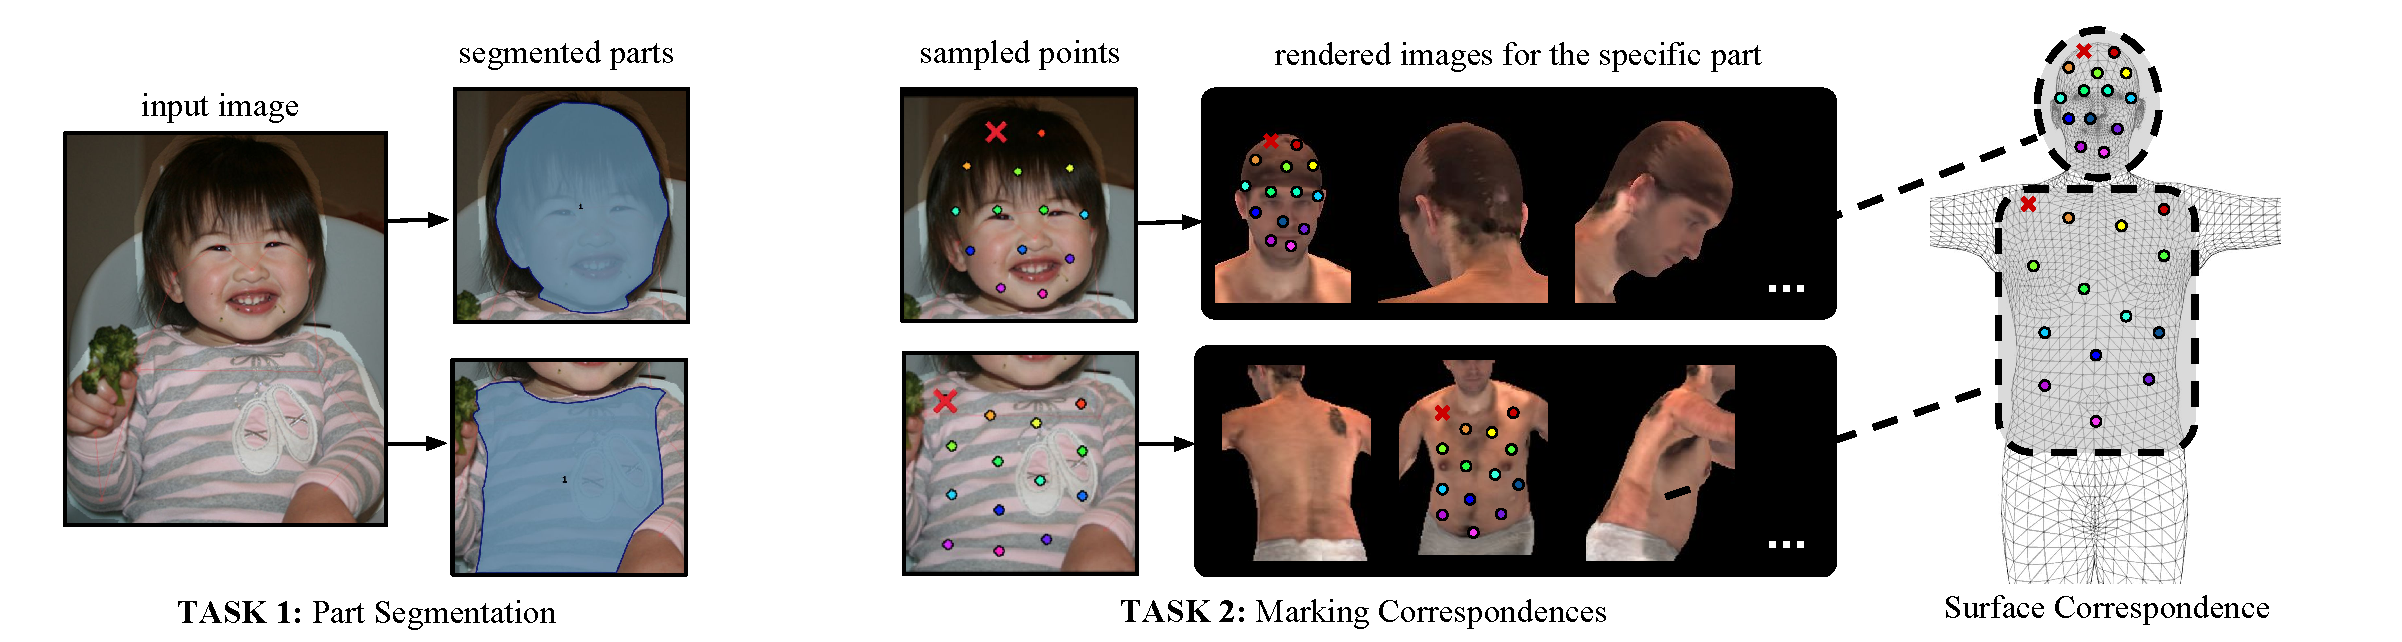
\includegraphics[width=0.8\linewidth]{pictures/DensePose.pdf}
    \caption{DensePose pipeline}
    \label{fig:DensePose}
\end{figure}

Despite its benefits (such methods overtake 2D methods in accuracy) 3D pose estimation faces significant challenges \cite{3D-pose-estimation-review}, mainly depth ambiguities when guessing 3D structure from 2D inputs and the shortage of large, real-world 3D datasets. First of all input types differ: with monocular (single image) 3D pose estimation being an unclear problem because many 3D poses can match a single 2D projection. To fix this, some methods directly predict 3D joint coordinates or estimate voxel-based probabilities for joints in a 3D space. Another common approach is to first find 2D poses and then "lift" them to 3D, such as using a neural network to learn this 2D-to-3D conversion or combining 2D joint heatmaps with 3D image clues. SMPL-based methods often adjust the model to match detected 2D keypoints, like in SMPLify \cite{SMPLify}, or directly predict SMPL parameters from image features. Using multiple camera views can greatly reduce depth uncertainty, however merging data from different cameras brings its own difficulties. Techniques here include combining 2D heatmaps from different views into a common 3D space, bringing consistency across multiple views, or using classical triangulation on 2D pose estimates \cite{3D-pose-estimation-review}. 


 \begin{figure}[h]
    \centering
    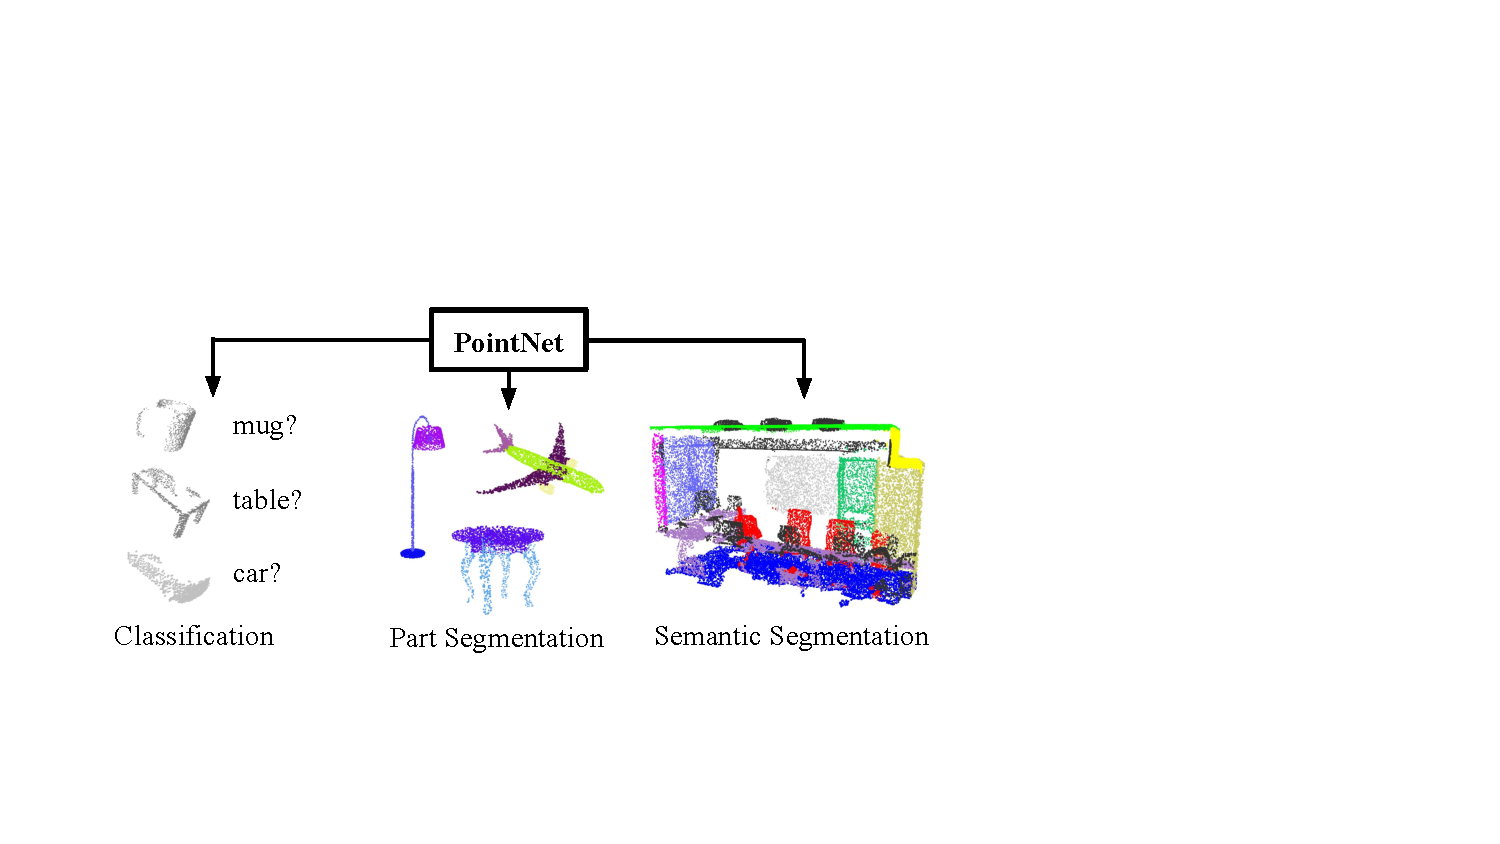
\includegraphics[width=0.8\linewidth]{pictures/point-net.pdf}
    \label{fig:PointNet}
\end{figure}

Beyond pose estimation, methods that directly process 3D point cloud data offer a powerful alternative for 3D Re-ID. \textbf{PointNet} \cite{PointNet} pioneered a deep learning architecture that takes in unordered point sets (groups of 3D coordinates, sometimes with extra details like color or normals Fig.~\ref{fig:PointNet}), respecting the permutation invariance of points in the input. Key features proposed by authors in PointNet is using a symmetric function (specifically max pooling), to aggregate information from individual point features into a global descriptor, ensuring that the network's output is invariant to the order of input points.
 The model learns to find and encode important points well. For tasks like segmentation—key for part-based Re-ID—PointNet mixes big-picture features with local point features, that point representation is aware of both its local geometry and the overall context of the shape. To deal with shape changes, PointNet uses \textbf{joint alignment networks (T-nets)} that predict transformation matrices to adjust input points and features, with a regularization term encouraging the feature transformation matrix to be orthogonal to preserve information. Working directly with raw point clouds skips errors from voxelization or multi-view rendering, and the model’s skill at learning from a few "critical points" (like an object’s skeleton) helps it handle noise and missing data—useful traits for Re-ID in messy, real-world settings.

This methods can be considered as further direction in my research, but currently there are not used. However I think they are worth to be mentioned, because this is powerful approach (in case i need more precise matching) in Re-ID \cite{reid_survey} and quite interesting in it's own. 

\subsection{Multimodal Person Re-ID Methods}

\textit{I found this method interesting, because it extends query-gallery matching on embeddings (typically appearance only) by introduction depth aware encoder model for generating embeddings.} This paper \cite{rgb-depth} addresses the challenge of cross-modal person re-identification (Re-ID) specifically between RGB (color-visual) and depth images. 

\paragraph{Purpose:} Main purpose is to investigate and propose a novel method for re-identifying individuals when one view is an RGB image and the other is a depth image. This idea becoming more relevant with cheap RGB-D cameras and sensor-heavy systems like self-driving cars. The core difficulty lies in the significant "modality gap" due to the different nature of information between RGB and depth sensors, in addition to standard Re-ID challenges like viewpoint changes, occlusions, and variations in pose and illumination.


\begin{figure}[h]
    \centering
    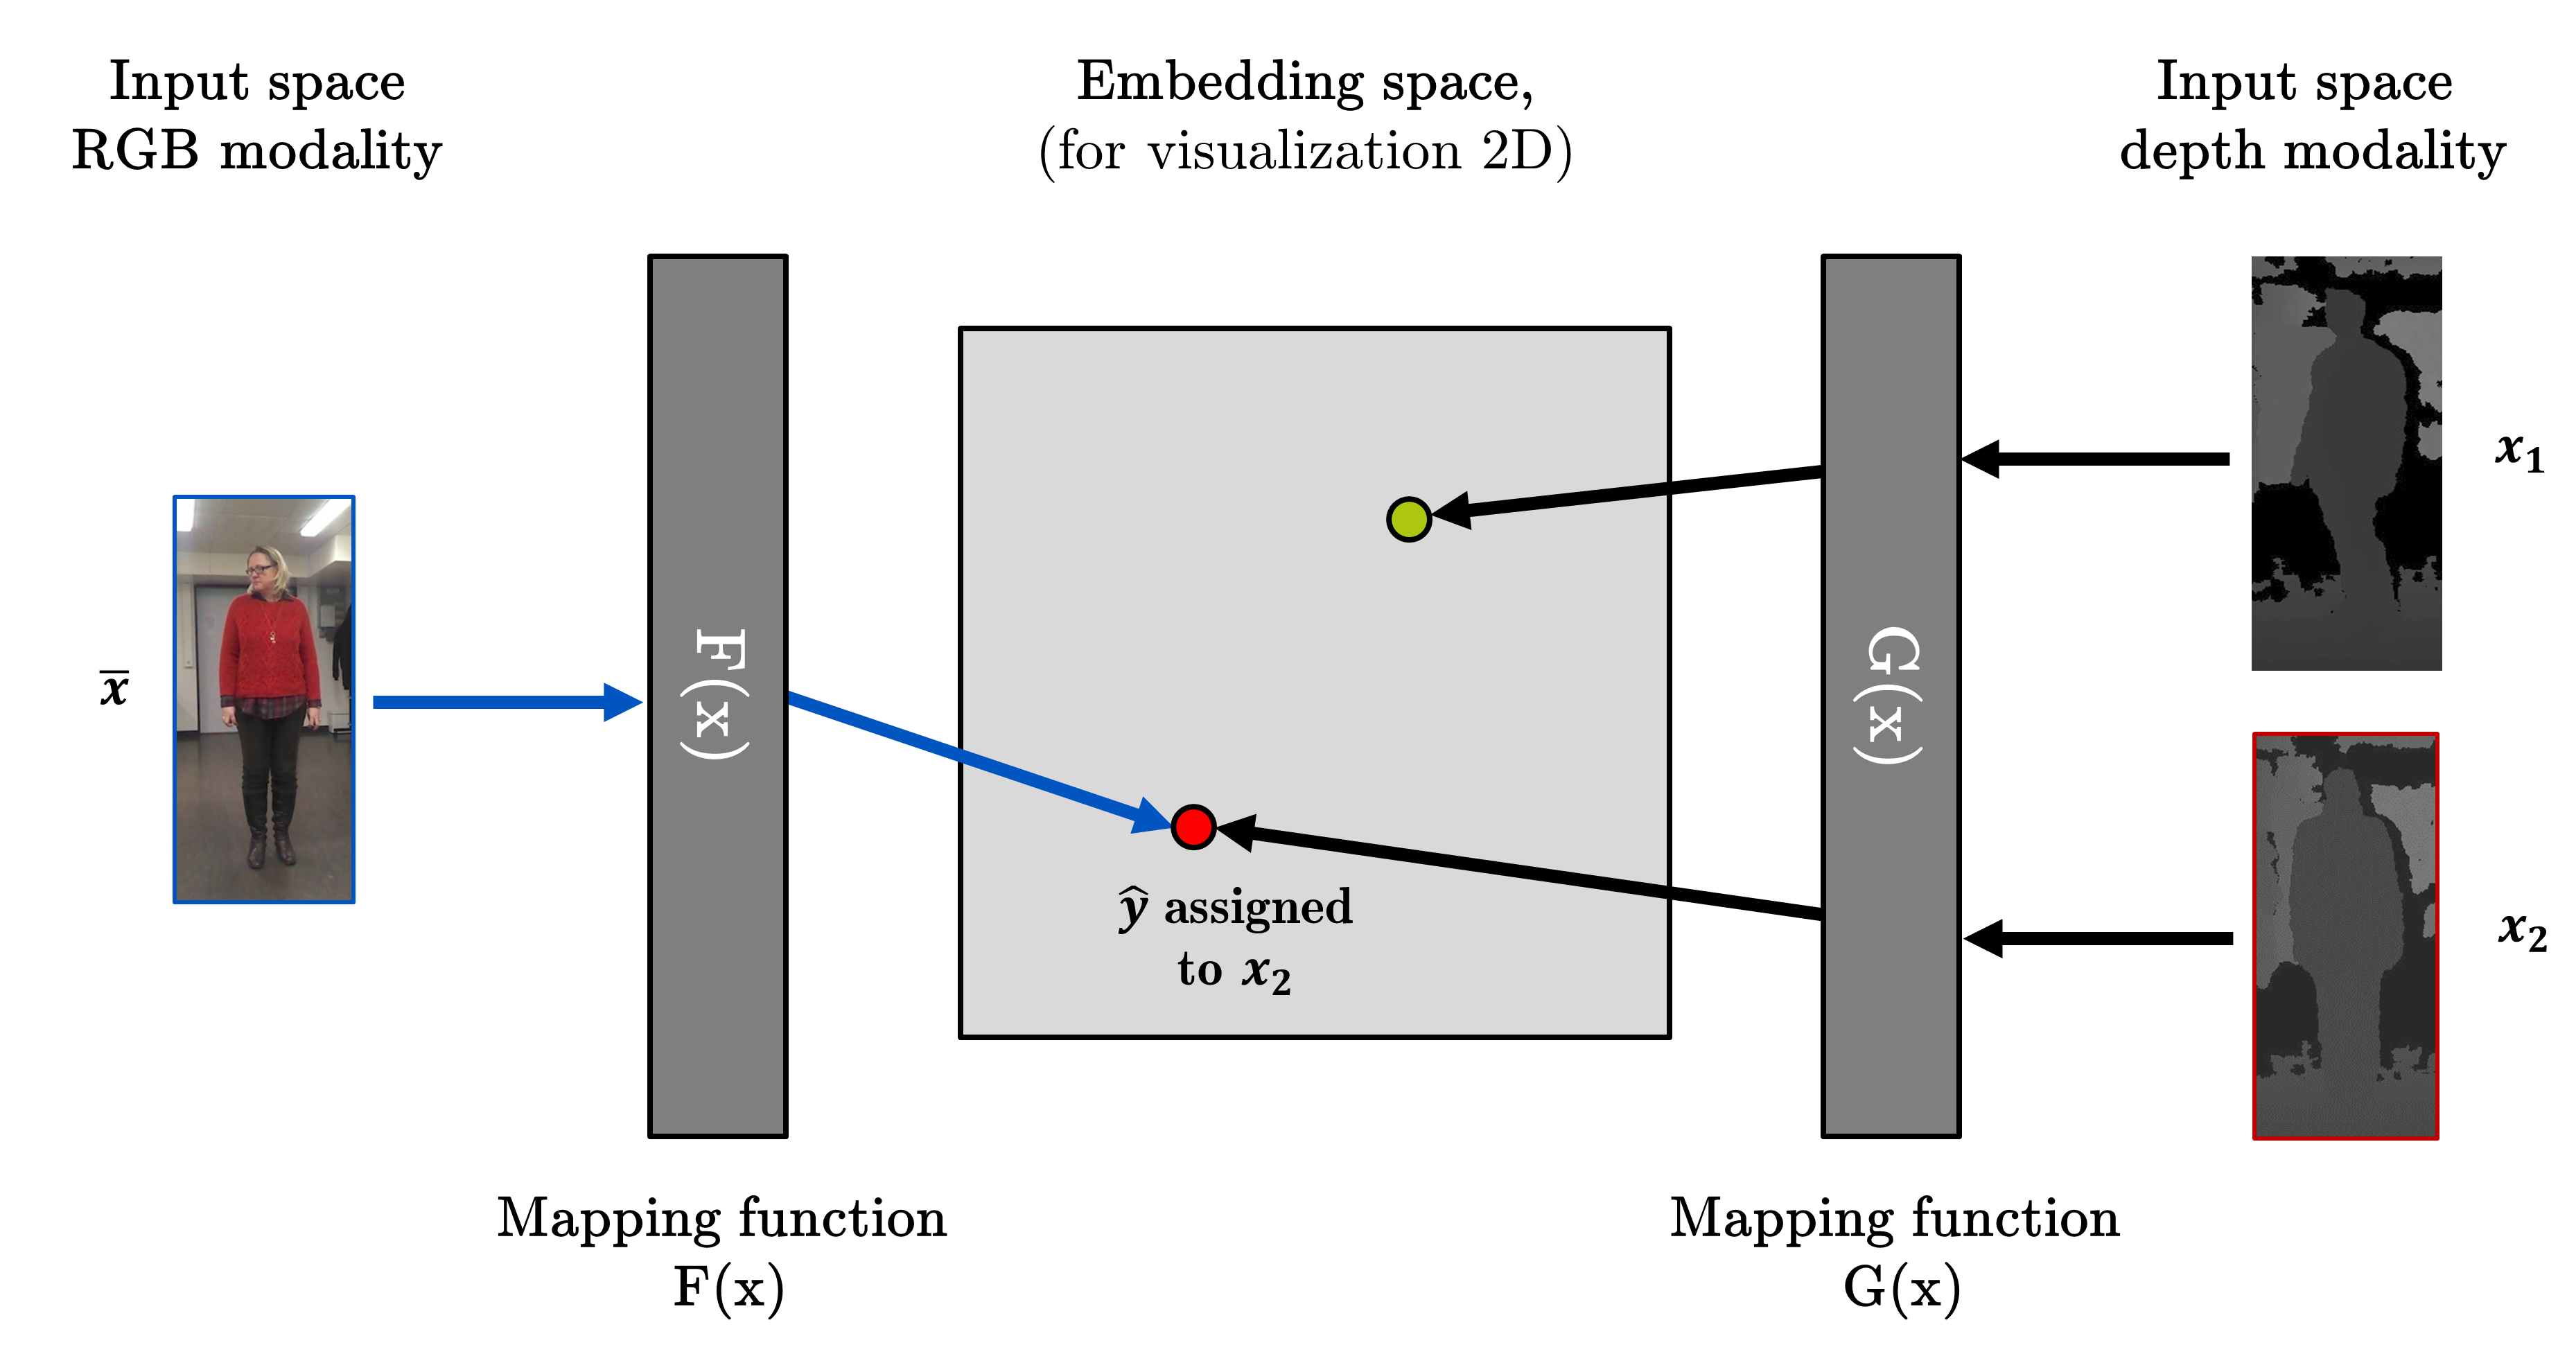
\includegraphics[width=0.6\linewidth]{pictures/depth-embed-match.png}
    \label{fig:depth-rgb-embed-match}
\end{figure}

\paragraph{Methods:} The key author's contribution is a two-step cross-modal distillation training procedure Fig.~\ref{fig:depth-scheme}.

\begin{enumerate}
	\item \textbf{Step I (Teacher Training)}: CCN, typically a ResNet50, is first trained for single-modal Re-ID on a "teacher" modality (e.g., depth images) using standard Re-ID losses like triplet loss or softmax loss.
	\item \textbf{Step II (Student Distillation):} The trained "teacher network" is then distilled into a "student" network for the second modality (e.g., RGB images). For that purpose, student network learns to mimic the feature embeddings or output distributions of the teacher network, effectively transferring the learned representation. The paper author's empirically investigates that distilling from depth (teacher) to RGB (student) yields superior performance.
\end{enumerate}
To further refine the feature representation, the authors propose integrating a \textbf{cross-modal gated attention mechanism} into the distillation process. During training, features from the teacher modality (depth) are used to generate a spatial attention map. Later, this attention map used to train the student network (RGB) by modulation its feature maps. This helps to focus on more relevant spatial regions and convolutional filters that align with the structural information present in the teacher modality (ref: Fig.~\ref{fig:depth-rgb-embed-match})


 \begin{figure}[h]
    \centering
    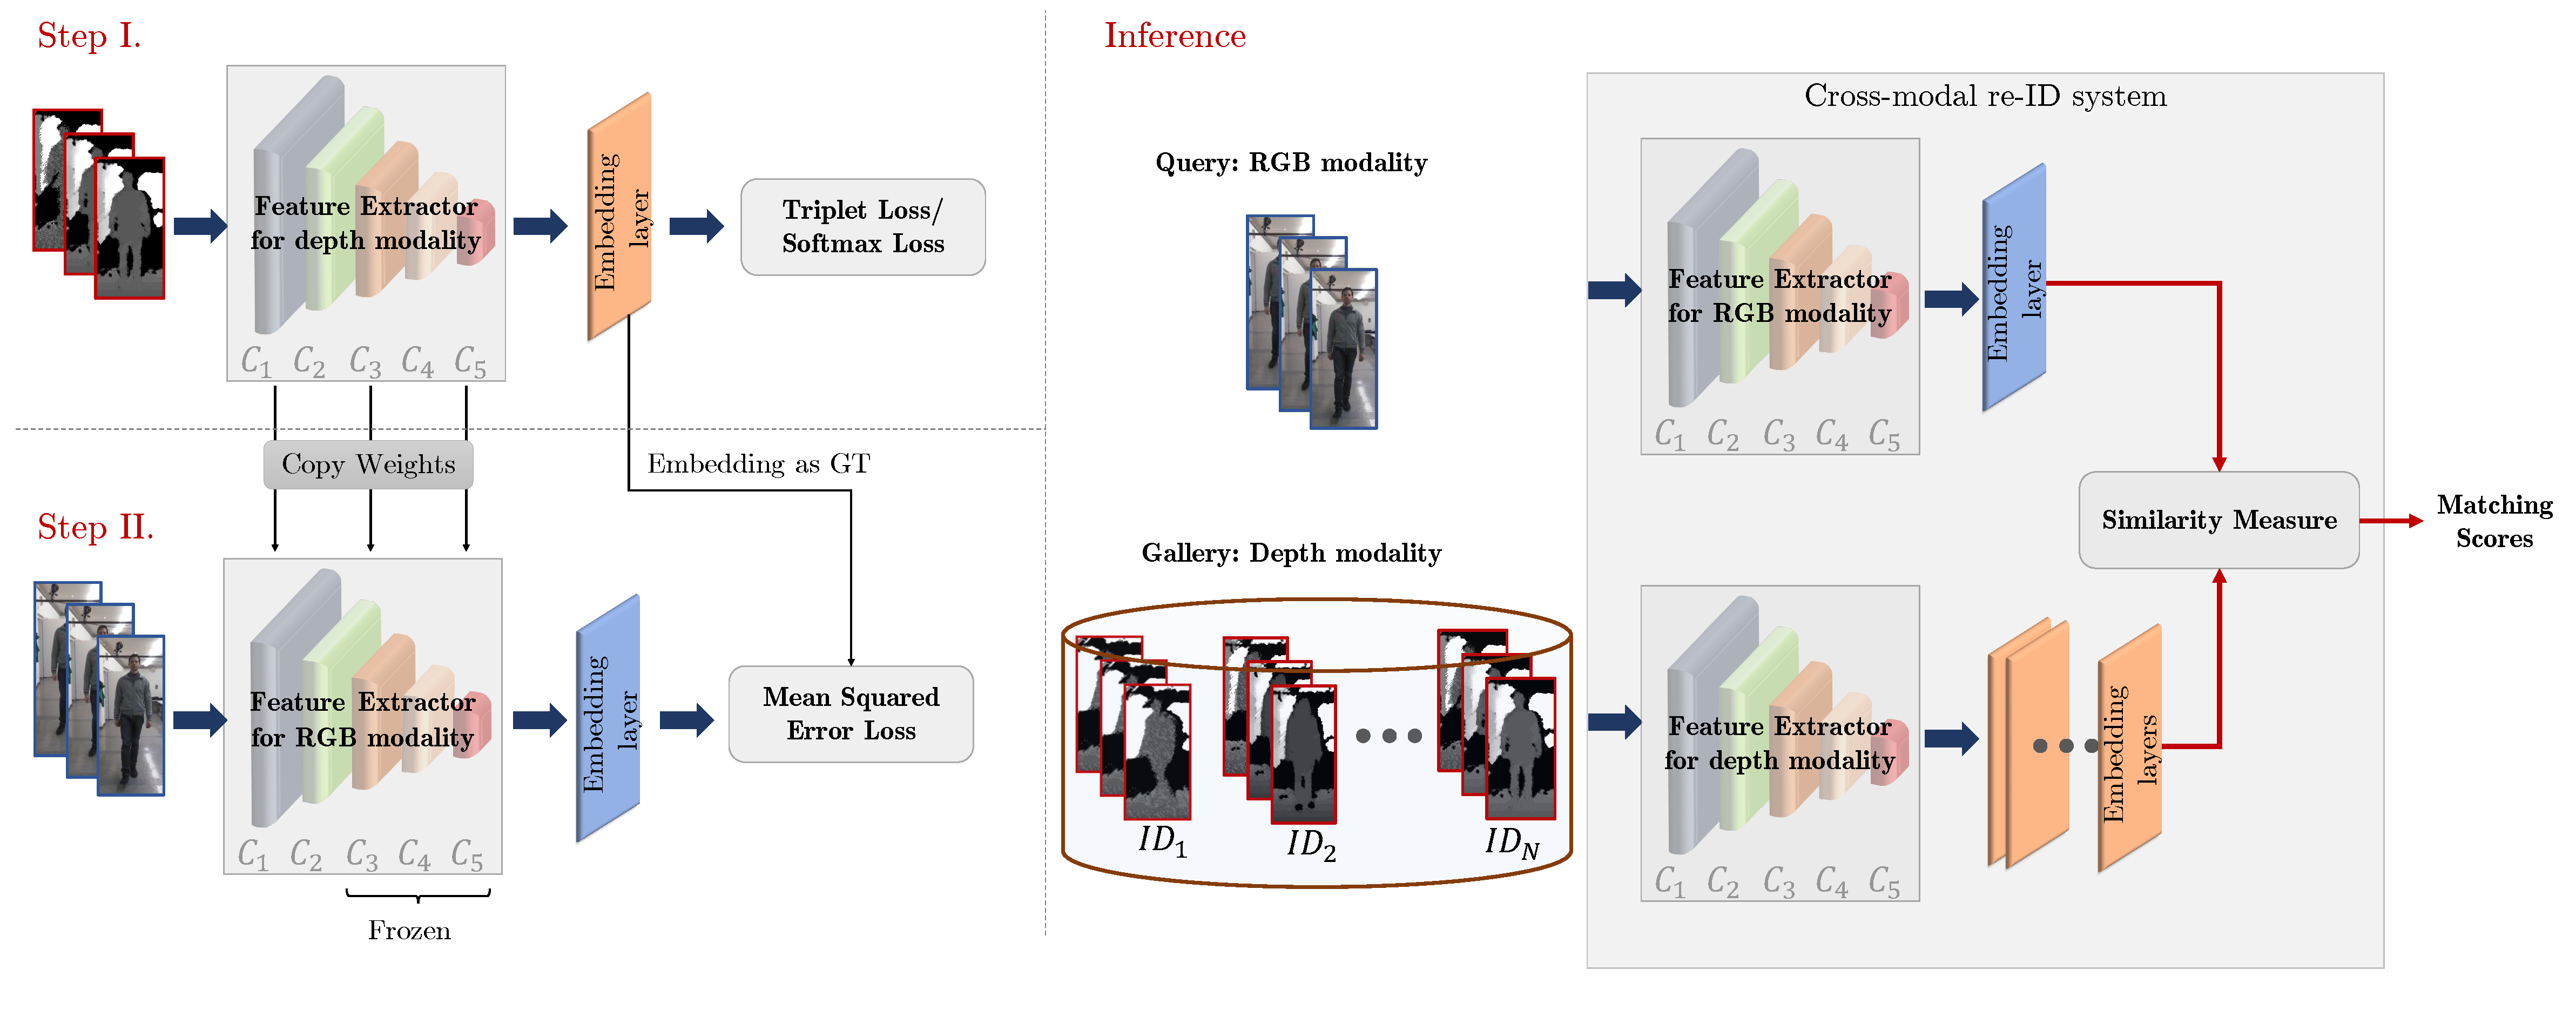
\includegraphics[width=0.9\linewidth]{pictures/depth-scheme.pdf}
    \caption{\textbf{RBG-Depth} training (left) and Inference (right) scheme: Step I involves training of a CNN for single-modal re-identification. In step II, the knowledge from the first modality is transferred to the second one. During inference, query and gallery images from different modalities are evaluated to produce feature embeddings and matching scores for cross-modal re-identification.}
    \label{fig:depth-scheme}
\end{figure}


\section{Related works: Cross-Camera Specific Re-ID}

\paragraph{Section Purpose:} 

This section reviews literature specifically addressing the challenges of cross-camera person Re-ID, which involves maintaining consistent identities across multiple camera views. This is complicated by changes in viewpoint, illumination, and occlusion. We examine key strategies—appearance-based methods, techniques for camera-invariant features, and the use of geometric constraints like homography—to contextualize this research's approach.

\subsection{Adversarial Camera Alignment Network (ACAN) for Unsupervised Cross-Camera Person Re-Identification \cite{ACAN}}


In this paper authors addressing matching individuals across non-overlapping camera views. They point the lack of labeled cross-camera data and propose a novel Unsupervised Cross-Camera (UCC) person Re-ID framework that utilizes only within-camera labels, which are easier to get through tracking and light manual labeling—avoiding the need for expensive cross-camera annotations. The main challenge in this setting is the distribution discrepancy across camera views, caused by differences in pose, occlusion, resolution, lighting, and background noise. Unlike traditional unsupervised methods that depend on pseudo-labels or external datasets, this approach only uses intra-camera data to fix this mismatch Fig.~\ref{fig:acan_inter_labeling}

\begin{figure}[h]
    \centering
    \begin{minipage}{0.45\textwidth}
        \centering
        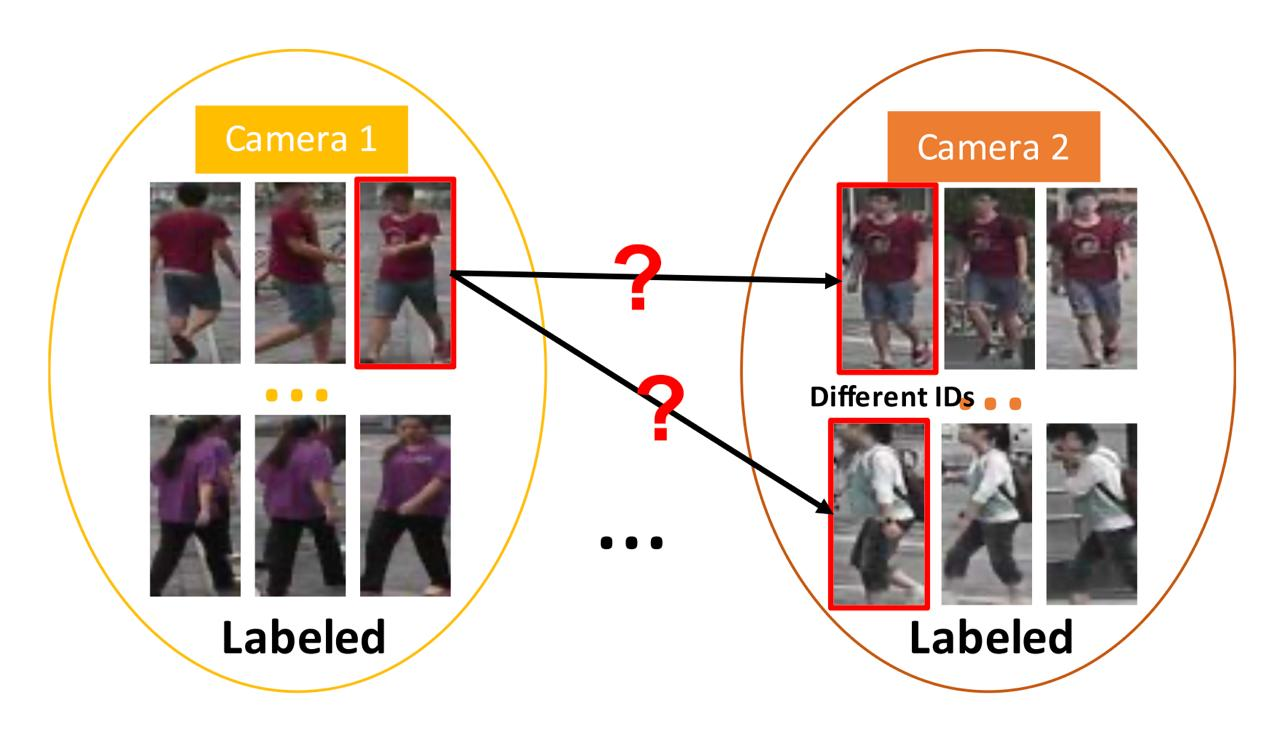
\includegraphics[width=\linewidth]{pictures/acan_inter_labeling}
        \caption{ACAN's setting of unsupervised “cross-camera” person Re-ID. Note that there is only two cameras at this  figure. As seen, we know the relationship of any two images from the same camera, while we do not have the label information of any two images from different cameras.}
        \label{fig:acan_inter_labeling}
    \end{minipage}
    \hfill
    \begin{minipage}{0.45\textwidth}
        \centering
        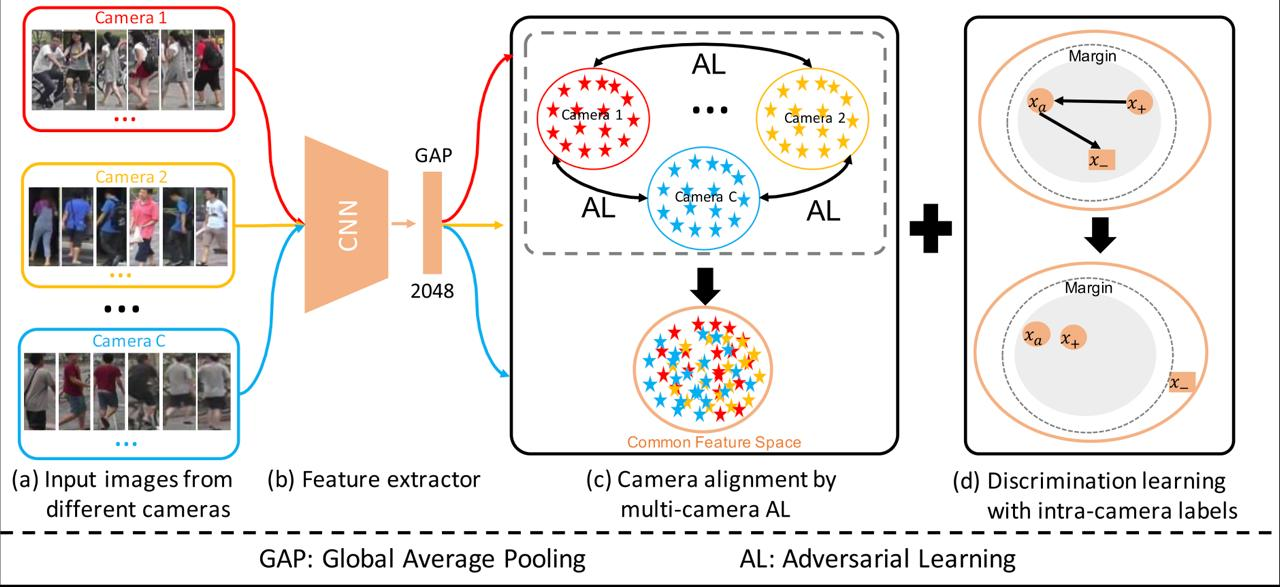
\includegraphics[width=\linewidth]{pictures/acan_pipe}
        \caption{An illustration of the proposed adversarial camera alignment network (ACAN).}
        \label{fig:acan_pipe}
    \end{minipage}
\end{figure}

To tackle this challenge, the authors introduce the Adversarial Camera Alignment Network (ACAN), which employs Multi-Camera Adversarial Learning (MCAL) to align the distributions of different cameras into a shared feature space Fig. ~\ref{fig:acan_pipe}. ACAN combines two primary tasks: a camera-alignment task and a supervised within-camera learning task. For alignment it employs the \textbf{Gradient Reversal Layer (GRL)}, a widely used technique that maximizes discriminator loss to improve camera distinctions, and a novel \textbf{"Other Camera Equiprobability"} (OCE) scheme. A new technique that forces the discriminator to treat all other cameras as equally likely (except the true one), preventing GRL’s "many-to-one" error in multi-camera cases. Extensive experiments on large-scale datasets demonstrate ACAN’s superiority over SOTA unsupervised methods that depend on labeled sources. 


\subsection{ReidTrack: Reid-only Multi-target Multi-camera Tracking \cite{Specker-ReID}}

Specker et al. 2023 present ReidTrack, a new method for multi-camera tracking that uses only appearance-based re-identification. This is usefull approach when camera setups or their spatial relationships (shared views, time-synchronization are unknown or hard to determine.

The main innovation is its multi-stage hierarchical clustering approach. For single-camera (inter-camera) tracking (reid), the system first handles non-overlapping detection using IoU-based tracking, if it's not enough it applies appearance-based clustering, and then, finally, deals with harder overlapping detections. Such step-by-step method better menages person-to-person occlusion. For cross-camera linking, ReidTrack extends the same clustering idea, using average appearance features to match identities across cameras. Simply using center of object features cluster, that is getting several crops of object, then extracting appearance features from them and take the mean across all dimensions for achieving average object embedding. 

A notable strength of ReidTrack is its computational efficiency. The authors achieve this through: 1. using YOLOv8 for detection, 2. frame downscaling, and  3. initial IoU-based tracking that reduces the load on the more computationally expensive re-identification steps. The paper demonstrates that appearance features alone can perform ReID task on non-complex scenes. 

\subsection{ReIDTrack - Multi-Object Tracking and Segmentation Without Motion \cite{reid-object-segmentaion}}

This work presents ReIDTrack, a tracking-by-detection system that breaks from traditional MOT methods (which use matching algorithms, like IoU and other \cite{SORT, DeepSORT, StrongSORT}) by using appearance features for matching, completely removing motion-based techniques (like Kalman filters) and IoU-based linking. The approach is driven by modern detectors' and re-ID models' improved cases where motion cues fail, such as low-FPS video or irregular motion patterns.

Authors uses their self-supervised appearance model (MoCo-v2 with ResNet50), which eliminates the need for costly tracking annotations during training (like was proposed in \cite{ACAN}. Their framework combines  CBNetV2 with Swin-B backbones (object detection model) with a simplified ByteTrack-inspired \cite{ByteTrack} association strategy, matching detections to tracklets solely through ReID distance (similarity between appearance embeddings). They also (as was proposed in \cite{Specker-ReID}) averaging features over tracklets, which reduce the computational cost and reduce features outliers from occlusion detections.

\begin{figure}[h]
    \centering
    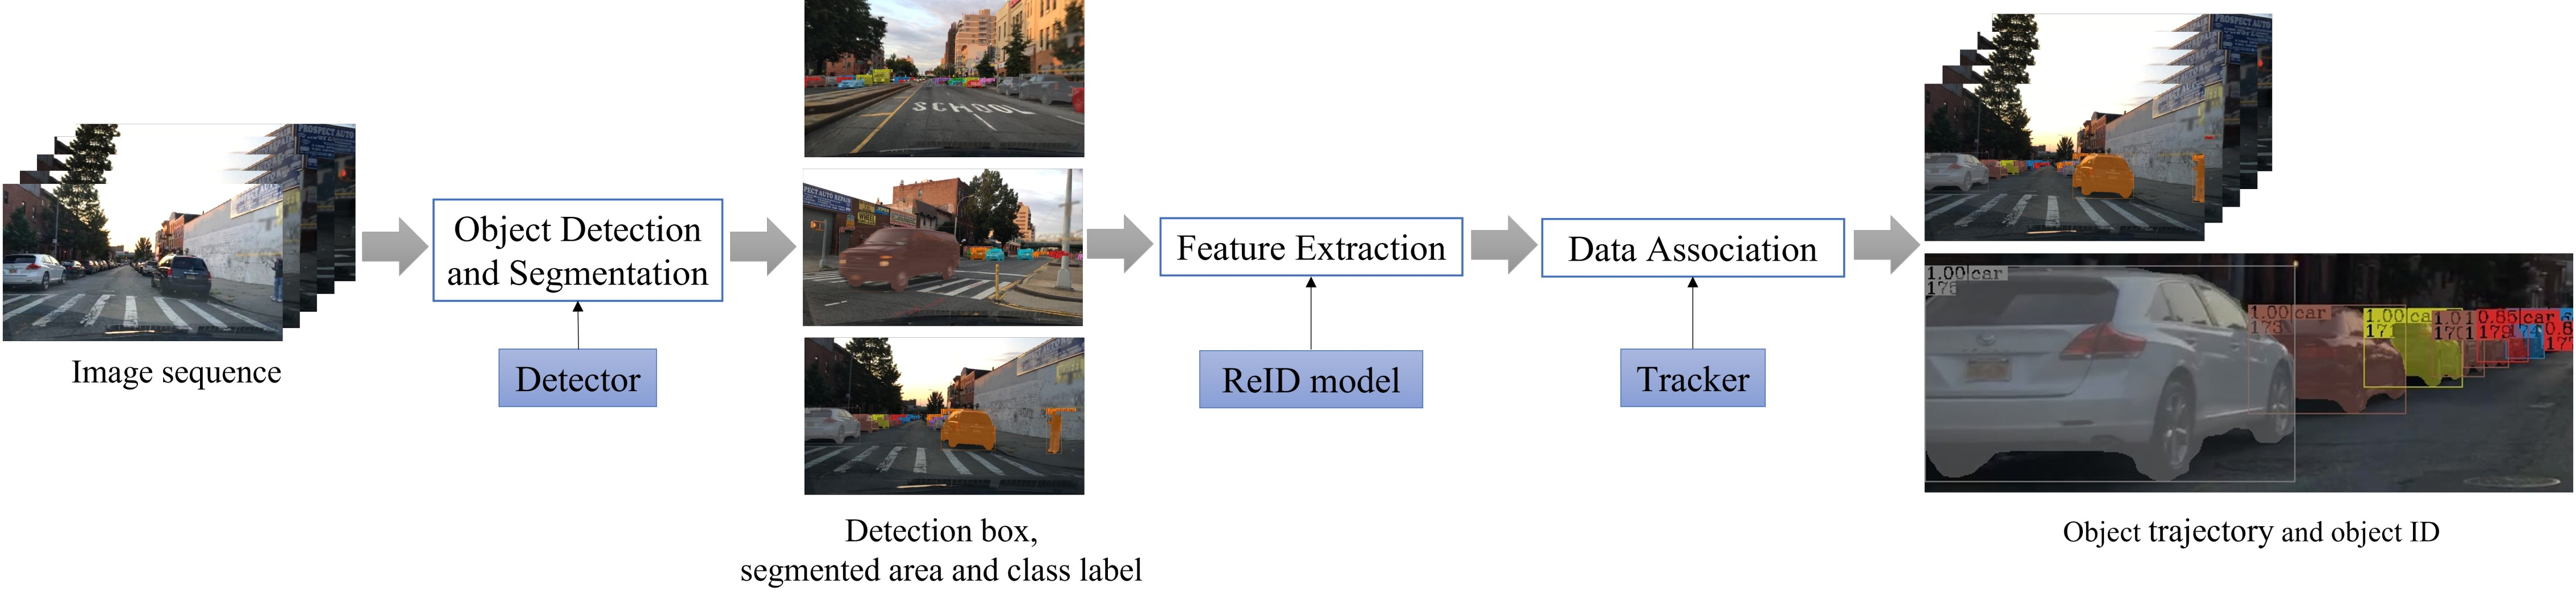
\includegraphics[width=0.95\linewidth]{pictures/no-motion-pipe}
    \caption{No-motion, segmentation-appearance-based ReID approach}
    \label{fig:no-motion-pipe}
\end{figure}

The authors demonstrate that appearance-only tracking can achieve SOTA-level performance (they take 1st place in the BDD100K MOTS challenge). Their results shows that motion cues, traditionally considered essential, may not be indispensable when paired with strong detection and ReID models. The findings point toward simpler, label-efficient tracking systems, especially where motion is hard to model.
 
\subsection{A Comprehensive Deep Learning Model for Improved Person Re-identification Using Multi-Camera Streaming Pipeline \cite{comp-dl-ReID}.}

To tackle Cross-Camera ReID problem, Patel et al. (2025) build a framework using SOTA components. Their methodology employs YOLOv8 \cite{yolov8} (which is not a cutting-edge model in fact in 2025, view corresponding section above), DeepSORT \cite{DeepSORT}, a MOT Tracking algorithm (which also isn't a SOTA solution in nowadays, for example \cite{ByteTrack, TransCenter, TransTrack, BoTsort, os-sort, StrongSORT}), but quite good custom transformer model built on the TorchReID framework: they utilize custom-trained OSNet (like in \cite{os-sort, deep-os-sort}) and ResNet50 models, which are fine-tuned on a blend of the Market 1501 dataset and a bespoke UNI09 dataset. The overall system achieves impressive (really impressive for such simple detection and tracking models) results, with OSNet attaining a 98.4\% mean Average Precision (mAP) and ResNet50 achieving 96.1\% mAP on the Market 1501 dataset.

However, when \textbf{I tested this approach} using different models, I was not able to get good results, due to a number of reasons. First, because I see each person for only a couple of seconds, I do not have time to collect a sufficiently diverse set of crops that show the same person in slightly different positions. Therefore at the second camera we view the same person with nothing common in appearance. For example on the first camera we see a man with his back turned to us, we see his black jacket and a brown briefcase on his back, on the next camera the man is facing the camera and we see his unzipped black jacket with a white T-shirt underneath. Visually these two observations are very different. Therefore, this approach is rather applicable for inter-camera reid tasks. However, since I have read many papers that use a similar purely visual method with several heuristics, I was obliged to test the applicability of this method on my own data.


\subsection{CLIP-ReID: Exploiting Vision-Language Model for Image Re-Identification without Concrete Text Labels \cite{clip-reid}}

This paper by Siyuan Li, Li Sun, and Qingli Li proposes a novel methodology which adapt the pre-trained vision-language model CLIP for image re-identification (ReID) tasks. Unlike traditional ReID approaches \cite{reid-object-segmentaion, reid_survey}, which rely on labeled dataset, in this paper the self-supervised learning from \cite{ACAN} was used. The authors introduce a two-stage training strategy that uses CLIP’s cross-modal features, achieving SOTA performance on various ReID datasets, including MSMT17, Market-1501, and VehicleID.

Vision-language models, such as CLIP (was originaly proposed by Radford et al. 2021 \cite{CLIP}) significantly excels CNN models in tasks like classification and segmentation by merging two modalities: natural language and visual. CLIP is a dual-encoder architecture trained to aligns image and text features in a shared embedding space. Prior adaptations of CLIP, such as CoOp (Zhou et al. 2021) \cite{CoOp-clip} for classification and DenseCLIP (Rao et al. 2022) \cite{dense-clip} for segmentation, propose to use task-specific prompts or fine-tuning, but not address ReID's challenge of non0semantic labels. Thankfully, this work \cite{clip-reid} fills this gap by introducing CLIP-ReID, a pioneering approach that re-purposes CLIP for ReID without concrete text labels Fig. ~\ref{fig:clip-reid-differ}

\begin{figure}[h]
    \centering
    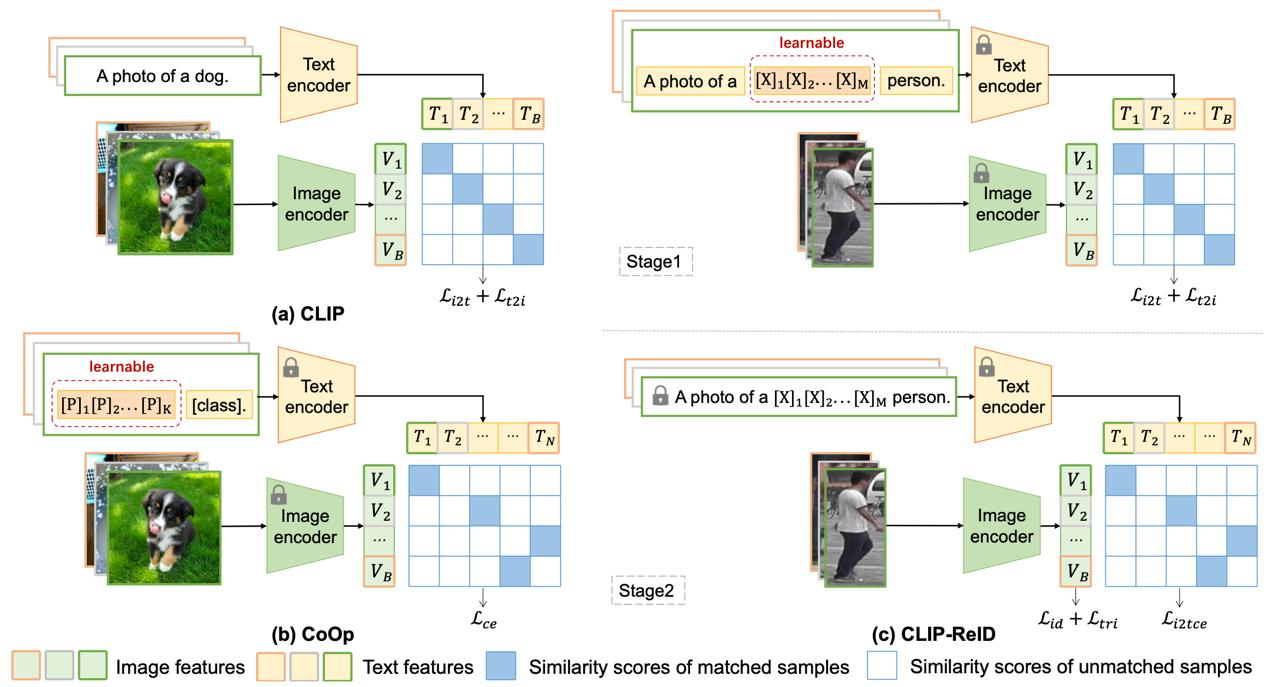
\includegraphics[width=0.95\linewidth]{pictures/clip-reid-differ.jpeg}
    \caption{Overview of the CLIP-ReID approach compared to CLIP and CoOp. (a) describes the model of CLIP, using pairs of text and image to train the image encoder and text encoder. (b) shows the model of CoOp, which fixes the image encoder and text encoder and fine-tunes text prompt in the downstream dataset. (c) is the proposed CLIP-ReID method, which fixes the text encoder and image encoder in the first training stage, optimizes a set of learnable text tokens to generate the text features, and then uses the text features to optimize the image encoder in the second training stage.}
    \label{fig:clip-reid-differ}
\end{figure}

The methodology, proposed by authors, hinges on a two-stage training strategy. In the first stage, authors train a ID-specific learnable text tokens to generate pseudo-textual descriptions, optimizing them using a contrastive learning, while preserving CLIP's pre-trained encoders. This approach allows the models itself to create identity-specific textual representations. The second stage fine-tunes CLIP's image encoder: it takes the text features learned in the first stage and uses them to guide the image encoder's training through multiple loss functions - the standard triplet loss and ID loss for ReID, plus a special cross-entropy loss that keeps the image features aligned with the text features. This introduce tow key technical improvements: side information embeddings (SIE) help the model to recognize when the same person appears under different cameras or viewpoint, and Overlapping Patches (OLP), which adjust how the model looks at image parts. This dual-stage process not only adapts CLIP’s cross-modal strengths to ReID but also outperforms state-of-the-art methods on datasets like MSMT17 (73.4\% mAP) and VehicleID (85.3\% mAP), as validated by extensive experiments and ablation studies. 

\begin{figure}[h!]
    \centering
    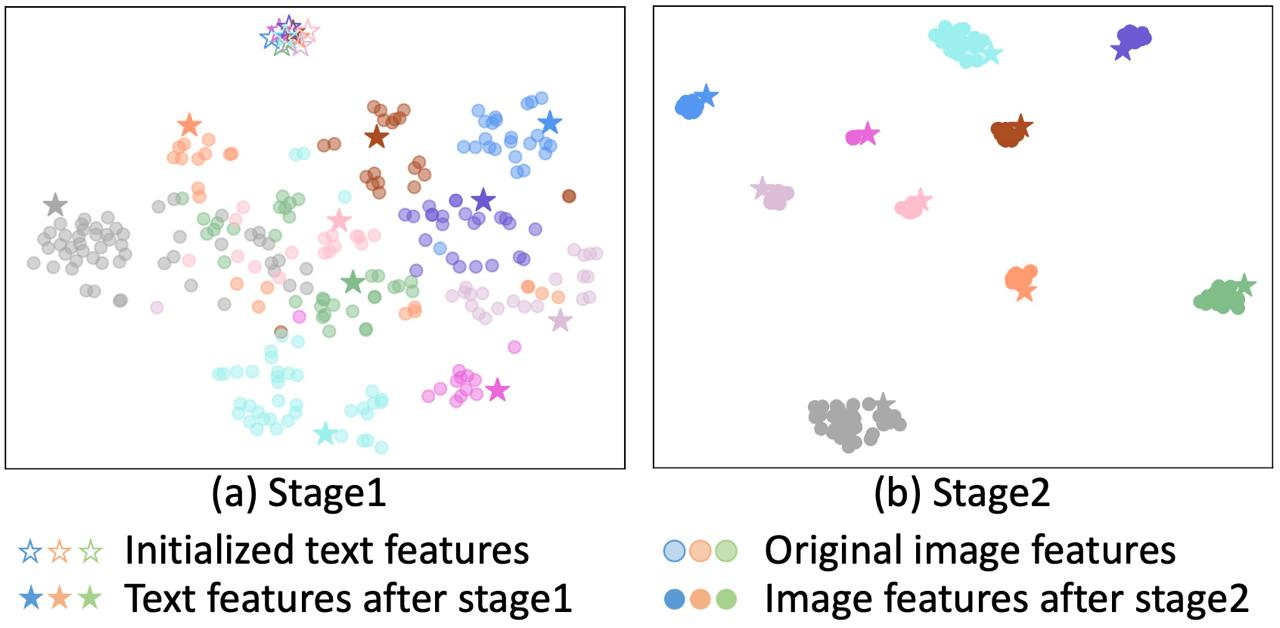
\includegraphics[width=0.65\linewidth]{pictures/clip-tsne.jpeg}
    \caption{t-SNE visualization on image and text features (Van der Maaten and Hinton 2008). Randomly selected 10 persons in the MSMT17 are represented by different colors. The dots and pentagons indicate the image and text features, respectively. (a) and (b) show the data distributions after the first and second training stage.}
    \label{fig:clip-tsne}
\end{figure}


Overall this structure leads to more discriminative feature extraction Fig.~\ref{fig:clip-tsne}. \textbf{I have also tried this approach}, and I can say that it worked noticeably better than the appearance only approach. However, its accuracy was still insufficient. Besides, with longer observation we will collect more and more data, adding more and more different people to our gallery, and the discriminativeness of the feature will be nullified, as there will be too many candidates (up to the point that we will see different people with exactly the same visual-descriptive representation).


\subsection{View-Centric Multi-Object Tracking with Homographic Matching in Moving UAV \cite{Homography-UAV}}

In this paper Deyi Ji et al. 2024 presents HomView-MOT designed to address the challenges of MOT in dynamic scenarios captured by moving Unmanned Aerial Vehicles (UAVs). Unlike traditional MOT methods (which are made for static or semi-static views) this framework handles drone movements like hovering, turning and altitude changes that cause major viewpoint shifts. The solution combines homography-based techniques with view-centric learning tacking with UAV datasets (VisDrone and UAVDT). 

The core of HomView-MOT lies in three innovative components: \textbf{Fast Homography Estimation} (FHE), \textbf{Homographic Matching Filter} (HMF), and \textbf{View-Centric ID Learning} (VCIL). FHE (using skip-frame sampling to reduce computation) efficiently calculates homography between frames Fig.~\ref{fig:UAV_homography}. HMF projects object boxes to a shared view plane for more accurate "physical IoU" matching instead of traditional IoU Fig.~\ref{fig:UAV_matching} VCIL employs \textbf{Homographic Slot Attention} (HSA) to learn better ID features across different viewpoints (for more comprehensive ReID embeddings). 

The method builds on standard tracking-by-detection (\hyperref[sec:Separate_Detection_Embedding]{SDE} and \hyperref[sec:Joint_detection_embedding]{JDE}) but enhances both detection and association stages. For detection, a shared network outputs boxes and ID features refined through VCIL. During association, HMF aligns boxes to a common view while VCIL improves feature matching.

\begin{figure}[h]
    \centering
    \begin{minipage}{0.5\textwidth}
        \centering
        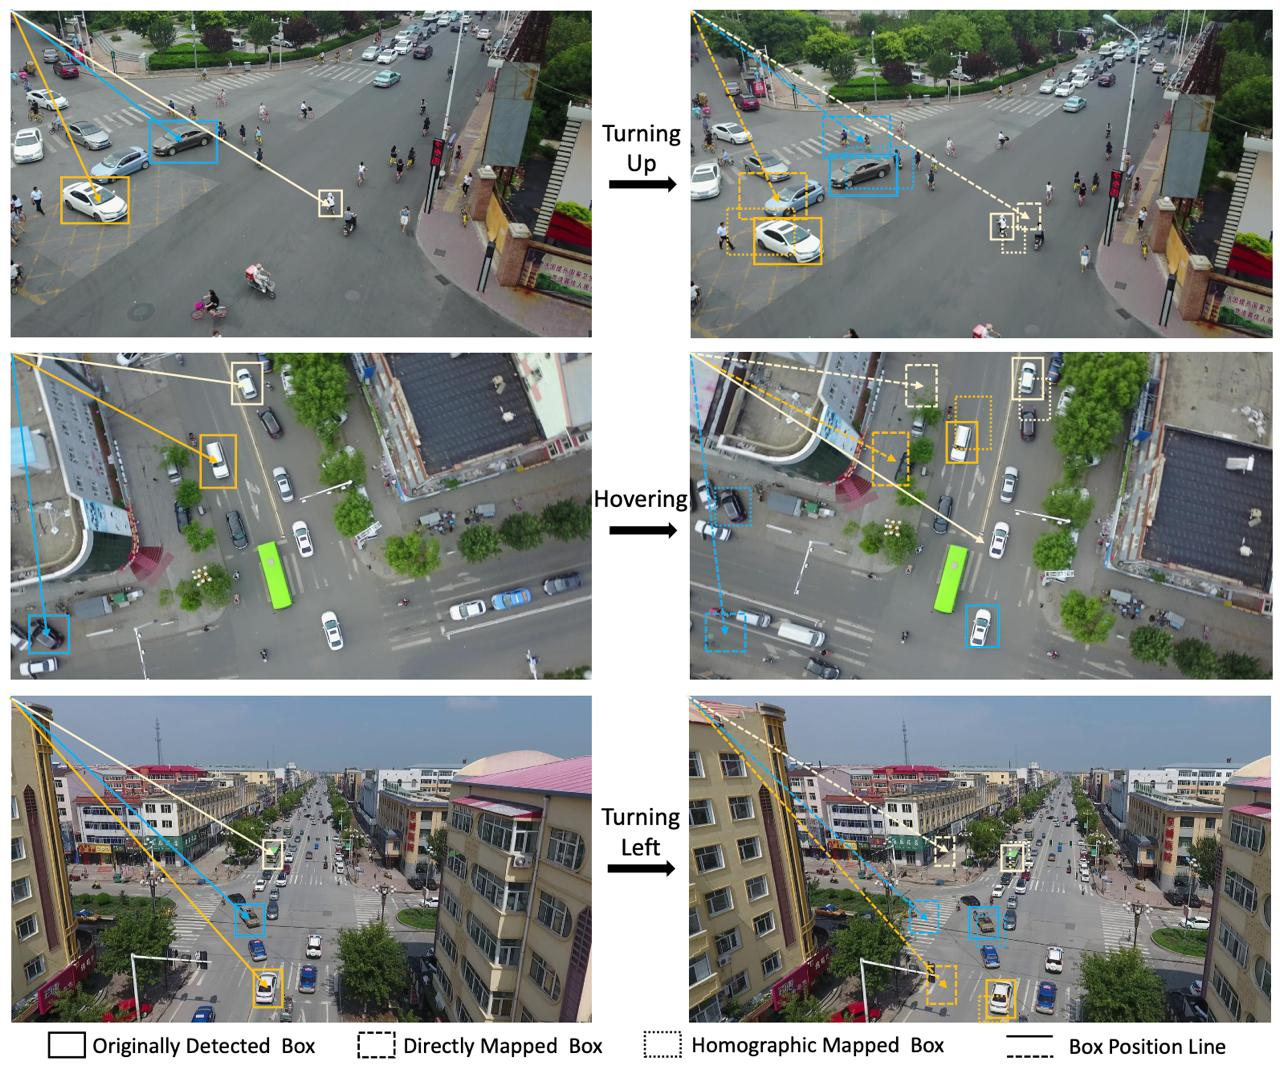
\includegraphics[width=\linewidth]{pictures/homography_UAV.jpeg}
        \caption{As seen, Homographic Matching Filter demonstrate better and more reasonable IoU association (relative to the real world) then traditional ordinary IoU association}
        \label{fig:UAV_matching}
    \end{minipage}
    \hfill
    \begin{minipage}{0.45\textwidth}
        \centering
        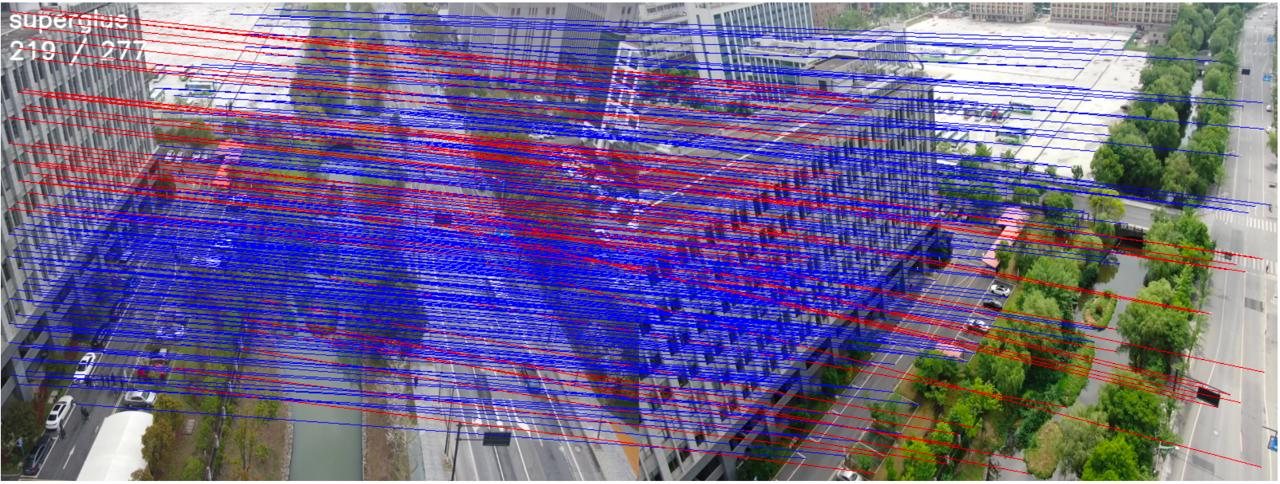
\includegraphics[width=\linewidth]{pictures/UAV_hom_map.jpeg}
        \caption{One example of the calculation of Homography matrix. The lines indicate the matching of key points between the two frames. Very old, therefore very fast HOG method.}
        \label{fig:UAV_homography}
    \end{minipage}
\end{figure}


Compared to existing work, HomView-MOT shows significant advantages. It outperforms UAVMOT's manual motion rules and works better than static-camera methods like \cite{DeepSORT, SORT, StrongSORT}. The homography-based HMF proves more robust than motion filters, while VCIL better handles viewpoint changes than standard ReID. 


\subsection{Applying multi layer homography for multi camera person tracking  \cite{multi-layer-homography}}
The paper "Applying Multi Layer Homography for Multi Camera Person Tracking" by Dejan Arsić \cite{multi-layer-homography} not explicitly designed for person re-identification (ReID), but propose multi-layer homography approach, which significantly enhances scene positioning and object association, which are critical for ReID tasks, especially in cross-camera settings. As was mentioned above matching individuals across different camera views, often hindered by occlusions, viewpoint changes, and appearance variations. The paper’s multi-layer homography tackles these issues by using more stable spatial localization. This approach use geometric constraints to significantly (in most cases absolutely) reducing the potential candidates set. Its focus on homography aligns with \cite{Homography-UAV}, which uses homography for multi-object tracking (MOT) in dynamic UAV scenarios, though Arsić et al. apply it to static multi-camera setups.

\paragraph{Methodology}
\emph{}
\textbf{1. Adaptive Foreground Segmentation}. Uses a Gaussian Mixture Model (GMM) to extract foreground blobs (\textit{Yes, its primitive, but it was in 2008 and still working)}, enhanced with shadow and highlight detection to reduce false positives Fig.~\ref{fig:shadow_detection}.

\begin{figure}[h]
    \centering
    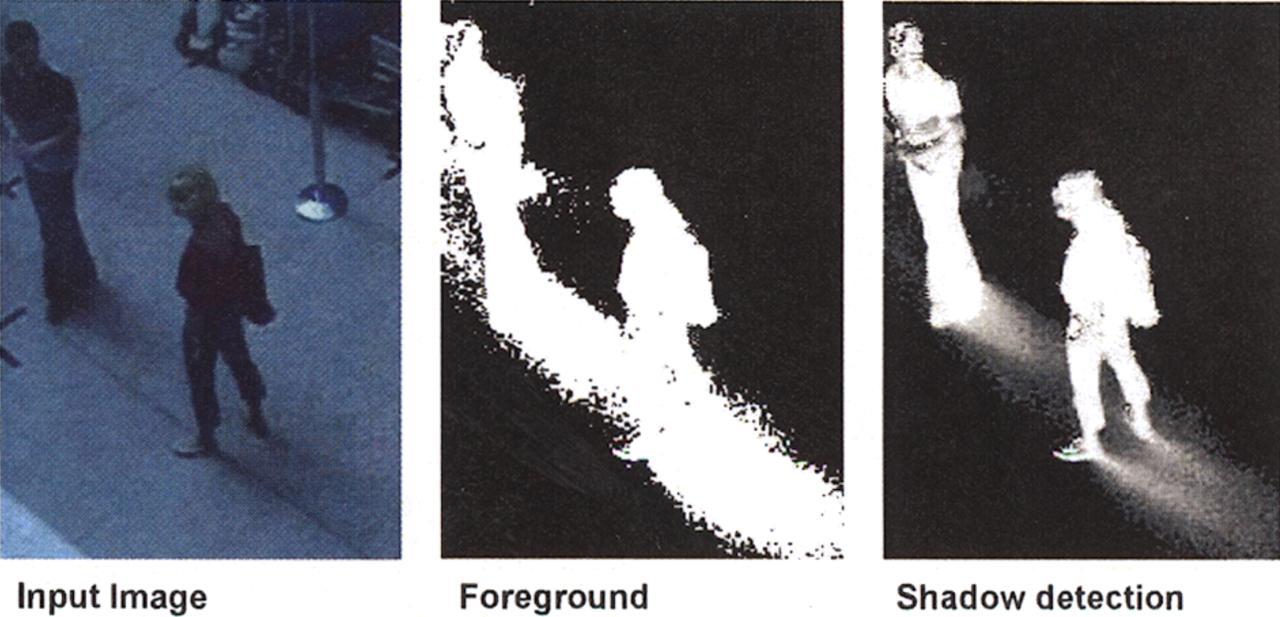
\includegraphics[width=0.65\linewidth]{pictures/shadow_detection.jpeg}
    \caption{Shadow detection in an image from PETS2007}
    \label{fig:shadow_detection}
\end{figure}

\textbf{2. Multi-Layer Homography for Object Detection}. Extends traditional (2D plane) homography (e.g., \cite{Homography-UAV}) by applying transformations across multiple height layers (0–2 meters), creating a pseudo-3D scene reconstruction. Blob boundaries from each camera are projected into layered planes, and intersections identify object positions. This reduce occlusion issues by using multiple perspectives, similar to how \cite{Homography-UAV} Homographic Matching Filter aligns objects in a shared view plane.


\begin{figure}[h]
    \centering
    \begin{minipage}{0.5\textwidth}
        \centering
        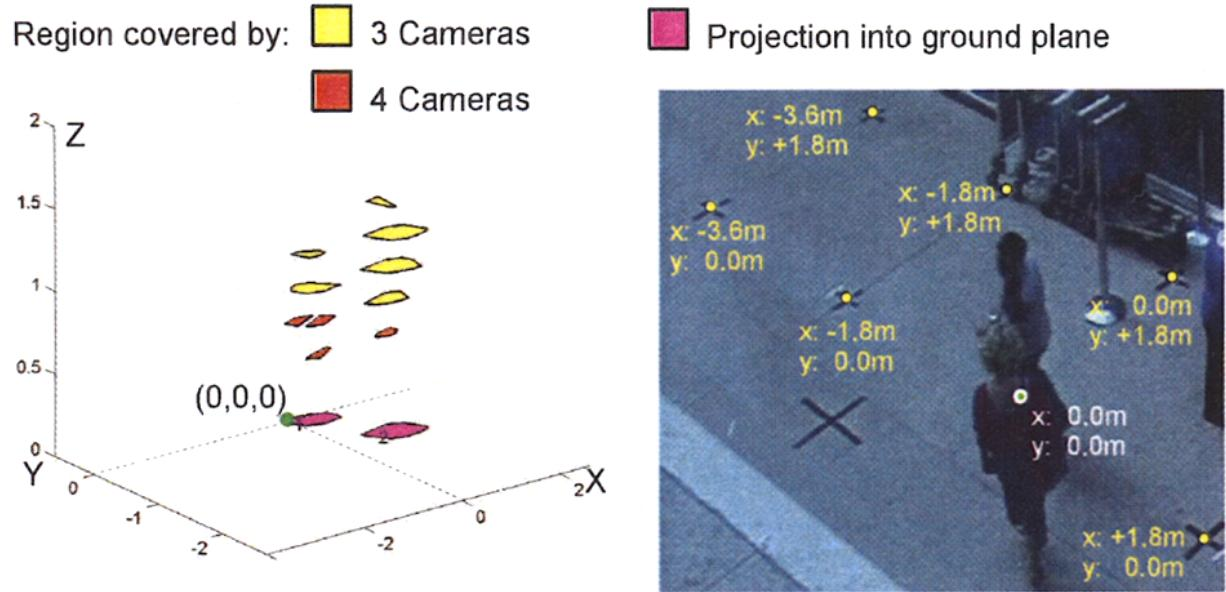
\includegraphics[width=\linewidth]{pictures/multi_layer_projections.jpeg}
        \caption{Exemplary multi layer transform in 6 layers and projection into the ground plane}
        \label{fig:multi_layer_projections}
    \end{minipage}
    \hfill
    \begin{minipage}{0.45\textwidth}
        \centering
        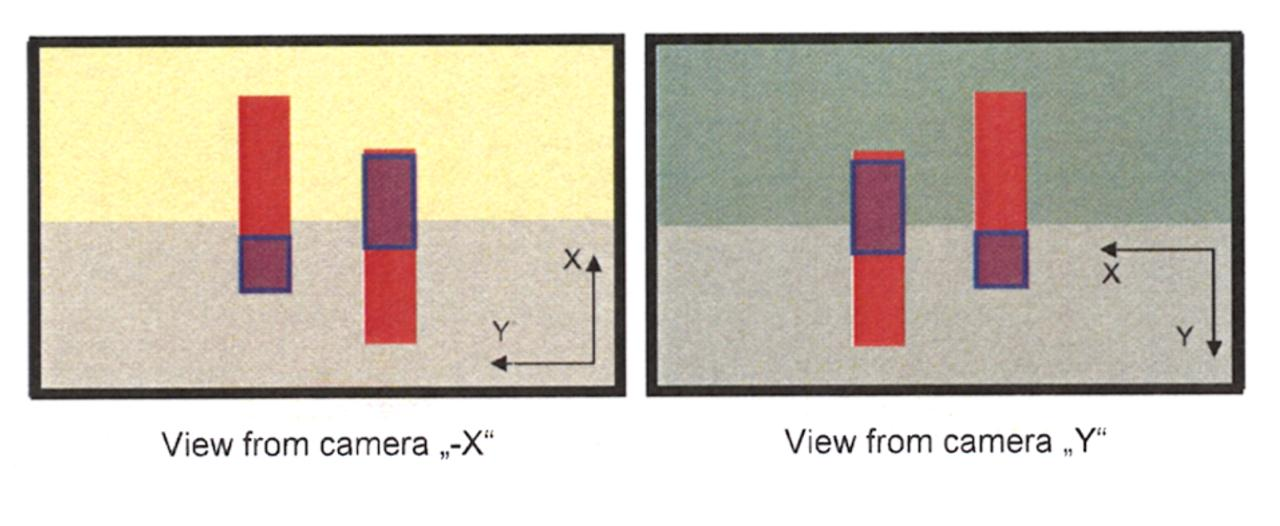
\includegraphics[width=\linewidth]{pictures/multi_layer_views.jpeg}
        \caption{All possible object positions are transformed back into 2D.}
        \label{fig:multi_layer_views}
    \end{minipage}
\end{figure}

 \textbf{3. False Positive Handling and Tracking} Back-projects 3D regions into 2D camera views to eliminate objects occluded in all perspectives, reducing false positives by 72\%. Employs a Kalman filter for trajectory prediction and SIFT features (it's 2008, so it is what it is) for identity resolution, akin to \cite{Homography-UAV} View-Centric ID Learning (VCIL) for feature matching across viewpoints.

\section{Research Objectives/Statement}

\subsection{Overview}

This research aims to design a system which constructs continuous trajectories for every visitor using a network of static, ceiling-mounted surveillance cameras. This data can be further utilized for analyzing customer movement within a shopping mall. For example for tracking conversion, behavioral pattern of buyers, areas of high interest and other business-useful statistics. Our cameras operate at 30 FPS, capture color footage, are time-synchronized, and include some with overlapping fields of view. No additional modalities (e.g., depth or point clouds \cite{rgb-depth, 3D-pose-estimation-review, PointNet}) are available. The primary goal is to generate continuous trajectories for every visitor across their entire visit. This problem is divided into two key sub-tasks:

\begin{enumerate}
	\item \textbf{Single-Camera Multiple Object Tracking}: Tracking all individuals within a single camera’s footage while maintaining their unique identities over time.
	\item \textbf{Cross-Camera Person Re-identification}: Linking the same individual across different cameras to form seamless, mall-wide trajectories. 
\end{enumerate}

\subsection{Single-Camera Multiple Object Tracking: Formalization}
\label{subsec:sigle-camera-formalization}

\paragraph{Input Space}
The input to the single-camera MOT system is a sequence of video frames from a single camera, along with associated metadata (e.g., timestamps).
\begin{itemize}
    \item \textbf{Frame Sequence}: Let $\mathcal{I} = \{I_1, I_2, \ldots, I_K\}$ denote the sequence of $K$ frames, where each frame $I_k$ at time $k$ is an image in the space $\mathcal{I}_k \subseteq \mathbb{R}^{H \times W \times C}$. Here, $H$ is the height, $W$ is the width, and $C=3$ is the number of color channels (RGB) for the 30 FPS color video.
    \item \textbf{Timestamps}: Each frame $I_k$ is associated with a timestamp $t_k \in \mathbb{R}_{\geq 0}$, assuming time synchronization across cameras. The sequence of timestamps is $\mathcal{T} = \{t_1, t_2, \ldots, t_K\}$, where $t_{k+1} - t_k \approx \frac{1}{30}$ seconds (for 30 FPS).
    \item \textbf{Input Space}: The input space is the Cartesian product of frame and timestamp sequences:
    \[
    \mathcal{S}_{\text{input}} = \mathcal{I} \times \mathcal{T} = \{ (I_1, t_1), (I_2, t_2), \ldots, (I_K, t_K) \}
    \]
    where each $(I_k, t_k) \in \mathbb{R}^{H \times W \times 3} \times \mathbb{R}_{\geq 0}$.
\end{itemize}

\paragraph{State Space}
The state of an object (person) in a frame describes its properties, such as position and velocity, in the context of tracking:
\begin{itemize}
    \item \textbf{Object State}: For the $j$-th person in frame $k$, the state is denoted $\mathbf{x}_k^j \in \mathcal{X}$, where $\mathcal{X}$ is the state space. Typically, the state includes:
    \begin{itemize}
        \item \textbf{Position}: The bounding box center $(c_x, c_y)$ in pixel coordinates
        \item \textbf{Size}: The width $w$ and height $h$ of the bounding box
        \item \textbf{Velocity}: Optional components $(v_x, v_y)$ for motion prediction.
    \end{itemize}
    Thus, the representation is:
    \[
    \mathbf{x}_k^j = [c_x, c_y, w, h, v_x, v_y]^T \in \mathbb{R}^6
    \]
    \textbf{Note:} in open-cv library bounding boxes described not by center coordinates + (w, h), but by coordinates of top-left corner of bounding box.
    \item \textbf{Frame States}: The collection of states for all $N_k$ persons in frame $k$ is:
    \[
    \mathbf{X}_k = (\mathbf{x}_k^1, \mathbf{x}_k^2, \ldots, \mathbf{x}_k^{N_k}) \in \mathcal{X}^{N_k}
    \]
    \item \textbf{Sequential States}: The states of the $j$-th person across frames $a$ to $b$ form a tracklet:
    \[
    \mathbf{x}_{a:b}^j = \{\mathbf{x}_a^j, \mathbf{x}_{a+1}^j, \ldots, \mathbf{x}_b^j\} \in \mathcal{X}^{b-a+1}
    \]
\end{itemize}

\paragraph{Measurement Space}
In the Tracking-by-Detection paradigm, measurements are derived from a detector (YOLO in my case). For the $j$-th person in frame $k$, the measurement $\mathbf{z}_k^j \in \mathcal{Z}$ typically includes:
    \[
    \mathbf{z}_k^j = [z_x, z_y, z_w, z_h, s]^T \in \mathbb{R}^5
    \]
    where $(z_x, z_y)$ is the bounding box center, $(z_w, z_h)$ is the width and height, and $s \in [0,1]$ is the detection confidence.
    All measurements in frame $k$ are:
    \[
    \mathbf{Z}_k = (\mathbf{z}_k^1, \mathbf{z}_k^2, \ldots, \mathbf{z}_k^{M_k}) \in \mathcal{Z}^{M_k}
    \]

\paragraph{Output Space (Tracklets)}
The output of the single-camera MOT system is a set of tracklets \textbf{$\mathcal{T} = \{ T^1, T^2, \ldots, T^J \}$}, where a tracklet for the $j$-th person is $ T^j = (id_j, \mathbf{x}_{a:b}^j) $ where $id_j \in \mathbb{N}$ is a unique identifier.


\paragraph{Appearance Features (ReID)}
For each detection $\mathbf{z}_k^j$, the ReID model extracts:
    \[
    \mathbf{f}_k^j \in \mathcal{F} = \mathbb{R}^d
    \]
    for further inter-camera appearance-based ReID

\subsection{Objective}
The objective is to estimate the optimal sequential states for all persons, formulated as a Maximum a Posteriori (MAP) estimation problem: 
\[
\mathbf{X}_{1:k}^* = \arg\max_{\mathbf{X}_{1:k}} p(\mathbf{X}_{1:k} | \mathbf{Z}_{1:k})
\]

 This seeks the most probable set of trajectories given all observed measurements.
 
 
 \subsection{Cross-Camera Person Re-identification: Formalization}
 
 \paragraph{Input Space} The input to the Cross-Camera ReID system consists of tracklets from multiple cameras, generated by the single-camera MOT pipeline (as formalized previously), along with camera metadata (e.g., timestamps and homography mappings.
 
 \begin{itemize}
 	\item \textbf{Cameras}: Let $\mathcal{C} = \{C_1, C_2, \ldots, C_M\}$ denote the set of $M$ cameras in the mall.
 	\item \textbf{Tracklets per Camera}: For camera $C_m$, the single-camera MOT system produces a set of tracklets:
 	\[
 	\mathcal{T}_m = \{ T_m^1, T_m^2, \ldots, T_m^{J_m} \}
 	\]
  where $T_m^j = (id_m^j, \mathbf{x}_{a:b}^{m,j})$ is the tracklet for the $j$-th person in camera $C_m$, with local ID $id_m^j \in \mathbb{N}$ and state sequence $\mathbf{x}_{a:b}^{m,j} = \{\mathbf{x}_a^{m,j}, \ldots, \mathbf{x}_b^{m,j}\} \in \mathcal{X}^{b-a+1}$. The state $\mathbf{x}_k^{m,j} \in \mathcal{X} = \mathbb{R}^6$ includes position, size, and velocity (e.g., $\mathbf{x}_k^{m,j} = [c_x, c_y, w, h, v_x, v_y]^T$).
  	
  	\item \textbf{Appearance Features}: Each tracklet $T_m^j$ is associated with a sequence of appearance features from the ReID model (e.g., OSNet):
  	\[
  	\mathbf{f}_{a:b}^{m,j} = \{\mathbf{f}_a^{m,j}, \ldots, \mathbf{f}_b^{m,j}\} \in \mathcal{F}^{b-a+1}
  	\]
  	where $\mathbf{f}_k^{m,j} \in \mathcal{F} = \mathbb{R}^d$ (e.g., $d=512$ for OSNet) is the feature embedding for the $j$-th person in frame $k$ of camera $C_m$.


	\item \textbf{Timestamps}: Each state $\mathbf{x}_k^{m,j}$ is associated with a timestamp $t_k^m \in \mathbb{R}_{\geq 0}$, synchronized across cameras (i.e., $t_k^m \approx t_k^n$ for cameras $C_m$ and $C_n$ at frame $k$).

	\item \textbf{Homography for Overlapping Cameras}: For a pair of cameras $(C_m, C_n)$ with overlapping fields of view, a homography matrix $H_{m,n} \in \mathbb{R}^{3 \times 3}$ maps pixel coordinates from camera $C_m$ to camera $C_n$. Let $\mathcal{H} = \{ H_{m,n} \mid (C_m, C_n) \text{ have overlapping views} \}$ denote the set of homography matrices.
 \end{itemize}
 
 Overall, the input space combines tracklets, appearance features, timestamps, and homography mappings:
  \[
  \mathcal{S}_{\text{input}} = \prod_{m=1}^M \mathcal{T}_m \times \prod_{m=1}^M \mathcal{F}_m \times \mathcal{T}_{\text{time}} \times \mathcal{H}
  \]
  where $\mathcal{F}_m = \{\mathbf{f}_{a:b}^{m,j} \mid T_m^j \in \mathcal{T}_m\}$ is the set of feature sequences for camera $C_m$, and $\mathcal{T}_{\text{time}} = \prod_{m=1}^M \{t_k^m \mid k=1, \ldots, K_m\}$ is the set of timestamps across all cameras.

\paragraph{Output Space}
The output of the Cross-Camera ReID system is a set of global tracklets, where tracklets from different cameras representing the same person are merged in one set and assigned a shared global ID.

A global tracklet for the $j$-th person is:
  \[
  T^j_{\text{global}} = (id_{\text{global}}^j, \{ T_{m_1}^{j_1}, T_{m_2}^{j_2}, \ldots, T_{m_p}^{j_p} \})
  \]
  where $id_{\text{global}}^j \in \mathbb{N}$ is a unique global ID, and $\{ T_{m_1}^{j_1}, \ldots, T_{m_p}^{j_p} \}$ is the set of camera-specific tracklets (from cameras $C_{m_1}, \ldots, C_{m_p}$) corresponding to the same person.

The set of all global tracklets is:
  \[
  \mathcal{T}_{\text{global}} = \{ T^1_{\text{global}}, T^2_{\text{global}}, \ldots, T^J_{\text{global}} \}
  \]
  where $J$ is the total number of unique persons in the mall. The output space is:
  \[
  \mathcal{S}_{\text{output}} = 2^{\mathbb{N} \times \bigcup_{m_1, \ldots, m_p} (\mathcal{T}_{m_1} \times \cdots \times \mathcal{T}_{m_p})}
  \]
  (the power set of global IDs paired with combinations of camera-specific tracklets).


\paragraph{Spatiotemporal Alignment (Homography-Based)}

\textbf{Coordinate Mapping.} For a tracklet state $\mathbf{x}_k^{m,j} = [c_x, c_y, w, h, v_x, v_y]^T$ in camera $C_m$, the position $(c_x, c_y)$ is mapped to camera $C_n$ using homography $H_{m,n}$:
  \[
  \begin{bmatrix} c_x' \\ c_y' \\ 1 \end{bmatrix} = H_{m,n} \begin{bmatrix} c_x \\ c_y \\ 1 \end{bmatrix}
  \]
  where $(c_x', c_y')$ are the homogeneous coordinates in camera $C_n$, normalized to Cartesian coordinates by dividing by the third component.

\textbf{Shared Coordinate Space}. Assume a common physical plane (here the mall floor). For each camera $C_m$, a homography $H_m$ maps pixel coordinates to a global coordinate system $\mathcal{G} = \mathbb{R}^2$. For a state $\mathbf{x}_k^{m,j}$, the global position is:
  \[
  \mathbf{g}_k^{m,j} = H_m ([c_x, c_y, 1]^T) \in \mathcal{G}
  \]

\textbf{Spatiotemporal Constraint}. Two tracklets $T_m^j = (id_m^j, \mathbf{x}_{a:b}^{m,j})$ and $T_n^i = (id_n^i, \mathbf{x}_{c:d}^{n,i})$ are candidates for the same person if, for some frame $k$ in their overlapping time interval $[t_{\max(a,c)}, t_{\min(b,d)}]$, their global positions are close:
  \[
  \| \mathbf{g}_k^{m,j} - \mathbf{g}_k^{n,i} \|_2 < \epsilon
  \]
  where $\epsilon$ is a spatial tolerance (e.g., 0.5 meters), and timestamps $t_k^m \approx t_k^n$ (due to synchronization) \textit{Details of matching algorithm explained in corresponding section}.

\paragraph{Appearance-Based Matching.}
For non-overlapping cameras or to refine spatiotemporal matches, appearance features are used:

\textbf{Feature Distance}: For tracklets $T_m^j$ and $T_n^i$, compute a similarity score (e.g., cosine similarity) between their feature sequences:
  \[
  s(\mathbf{f}_{a:b}^{m,j}, \mathbf{f}_{c:d}^{n,i}) = \frac{1}{L} \sum_{k \in \text{overlap}} \frac{\mathbf{f}_k^{m,j} \cdot \mathbf{f}_k^{n,i}}{\|\mathbf{f}_k^{m,j}\|_2 \|\mathbf{f}_k^{n,i}\|_2}
  \]
  where $L$ is the number of overlapping frames, and $s \in [-1, 1]$. A threshold $\theta_{\text{appearance}}$ (e.g., 0.8) determines a match.


\paragraph{Objective.}
The Cross-Camera ReID problem is to assign global IDs to tracklets by solving a clustering problem: 
\[
\mathcal{T}_{\text{global}}^* = \arg\max_{\mathcal{T}_{\text{global}}} p(\mathcal{T}_{\text{global}} | \mathcal{T}_1, \ldots, \mathcal{T}_M, \mathcal{H}, \{\mathbf{f}_{a:b}^{m,j}\})
\]
This can be formulated as minimizing an energy function:
\[
\mathcal{T}_{\text{global}}^* = \arg\min_{\mathcal{T}_{\text{global}}} E(\mathcal{T}_{\text{global}} | \mathcal{T}_1, \ldots, \mathcal{T}_M, \mathcal{H}, \{\mathbf{f}_{a:b}^{m,j}\})
\]
where the energy function $E$ includes:

\textbf{Spatiotemporal Term}: Penalizes mismatches in global coordinates and timestamps for overlapping cameras.
  \[
  E_{\text{st}} = \sum_{(m,n) \in \mathcal{H}} \sum_{k} \sum_{(j,i)} \mathbb{1}_{t_k^m \approx t_k^n} \cdot \max(0, \| \mathbf{g}_k^{m,j} - \mathbf{g}_k^{n,i} \|_2 - \epsilon)
  \]
  
  \textbf{Appearance Term}: Penalizes dissimilar features for tracklet pairs assigned the same global ID.
  \[
  E_{\text{app}} = \sum_{T^j_{\text{global}}} \sum_{(T_m^a, T_n^b) \in T^j_{\text{global}}} (1 - s(\mathbf{f}_{a:b}^{m,a}, \mathbf{f}_{c:d}^{n,b}))
  \]
  
  \textbf{Consistency Term}: Ensures each tracklet belongs to exactly one global tracklet.
  
\paragraph{Optimization Framework}
The energy minimization problem can be solved using a \textbf{graph-based clustering approach} (e.g. K-Means) :

 \textbf{Nodes}: Camera-specific tracklets $T_m^j$.

 \textbf{Edges}: Connect tracklets with high spatiotemporal or appearance similarity.

 \textbf{Objective}: Partition the graph into clusters, each representing a global tracklet $T^j_{\text{global}}$, minimizing $E$.

Alternatively, a probabilistic approach can model the joint probability:
\[
p(\mathcal{T}_{\text{global}} | \mathcal{T}_1, \ldots, \mathcal{T}_M, \mathcal{H}, \{\mathbf{f}_{a:b}^{m,j}\}) \propto \prod_{T^j_{\text{global}}} p_{\text{st}}(T^j_{\text{global}} | \mathcal{H}) \cdot p_{\text{app}}(T^j_{\text{global}} | \{\mathbf{f}_{a:b}^{m,j}\})
\]
where $p_{\text{st}}$ and $p_{\text{app}}$ are likelihoods for spatiotemporal and appearance consistency, respectively.

\paragraph{Mapping to Global Tracklets}
The ReID system maps the input $\mathcal{S}_{\text{input}}$ to the output $\mathcal{S}_{\text{output}}$ via a function:
\[
\Psi: \mathcal{S}_{\text{input}} \to \mathcal{S}_{\text{output}}
\]

where $\Psi(\{\mathcal{T}_m\}, \{\mathbf{f}_{a:b}^{m,j}\}, \mathcal{T}_{\text{time}}, \mathcal{H}) = \mathcal{T}_{\text{global}}$. 


\section{Methodology: Single-Camera Multiple Object Tracking.}

\subsection{Components}
Since the Tracking by Detection (\textbf{TBD}) approach prove it’s effectiveness \ref{MOT_paradigms_table} and it's well-integrated, I choose this paradigm. Offline methods excels in accuracy, they was too costly in the computational sense for me. Therefore I was pushed to use \textbf{online} methods. 

As a detection model I choose \textbf{YOLOv12} since it’s best SOTA solution available according to COCO benchmark. \ref{detectionModelTable} 

As a tracker I’ve tried BotSORT \cite{BoTsort}, ByteTrack \cite{ByteTrack} and DeepSORT \cite{DeepSORT}. According to my literature review block and MOT20 benchmark, BotSORT and ByteTrack excels old DeepSORT (despite I appreciate it’s integration). At the end I decide to choose BotSORT, because it excels in crowded-dense scenarios. 

And as the inter-camera ReID model for ByteTrack I choose OSNet model. According to my literature review block Omni-Scale Network is overperform most of ReID inter-camera models (at least at its size, because inference of CLIP models was painful.  Also it's well-integrated in TorchREID library, which significantly simplified my life.

This pipeline considered is SOTA in 2025, however doesn’t bring novelty. Therefore let’s move to post-processing heuristics.







\subsection{Post-processing ReID to Mitigate Identity Switches}

Despite the integration of a robust ReID model (OSNet) within our single-camera MOT pipeline (YOLOv12, BoT-SORT), the nature of online, detection-based tracking can still lead to identity switching, particularly when individuals remain occluded for extended periods (e.g., more than 2 seconds). When an object reappears after such an occlusion, the tracker might assign it a new ID, fragmenting its trajectory. To address this, we implement a post-processing ReID step aimed at re-associating these fragmented tracklets.

The fundamental approach for this intra-camera ReID post-processing is analogous to the appearance-only strategy detailed for cross-camera ReID (see Section 7.1: Attempts of Using Appearance-Only Approach), adapted here for re-linking tracklets within the same camera view. The core idea is to use a query-gallery framework based on visual appearance features.

\subsubsection{Methodology}

When a tracklet, say $T_{A}$, terminates (e.g., due to occlusion or temporarily leaving the frame) and shortly thereafter a new tracklet, $T_{B}$, initiates in a spatially proximate region, $T_{A}$ becomes a "query" and $T_{B}$ (along with other newly initiated tracklets in the vicinity) forms a "gallery" of candidates for re-association.

\begin{enumerate}
    \item \textbf{Feature Extraction and Aggregation:}
    \begin{itemize}
        \item For the query tracklet $T_{A}=(id_{A}, x_{a:b}^{A}, f_{a:b}^{A})$, which ended at frame $b$, we consider its appearance features $f_{k}^{A}$ from its last few observed frames. These are aggregated into a representative feature vector $\overline{f}^{A}$ using averaging, similar to Equation 4:
        $$ \overline{f}^{A} = \frac{1}{N_A} \sum_{k=b-N_A+1}^{b} f_{k}^{A} $$
        where $N_A$ is the number of recent frames from $T_A$ used for representation.

        \item For each candidate tracklet $T_{B}=(id_{B}, x_{c:d}^{B}, f_{c:d}^{B})$ in the gallery, which started at frame $c$, we use its initial appearance features $f_{k}^{B}$. These are similarly aggregated into $\overline{f}^{B}$:
        $$ \overline{f}^{B} = \frac{1}{N_B} \sum_{k=c}^{c+N_B-1} f_{k}^{B} $$
        where $N_B$ is the number of initial frames from $T_B$ used.
    \end{itemize}

    \item \textbf{Similarity Scoring:}
    The similarity between the query tracklet $T_A$ and a candidate tracklet $T_B$ is computed using the cosine similarity between their aggregated feature vectors:
    $$ s(\overline{f}^{A}, \overline{f}^{B}) = \frac{\overline{f}^{A} \cdot \overline{f}^{B}}{\|\overline{f}^{A}\|_{2} \|\overline{f}^{B}\|_{2}} $$
    This score $s \in [-1, 1]$ indicates the visual similarity, with higher values suggesting a stronger match.

    \item \textbf{Matching and Merging:}
    A match is confirmed if the similarity score $s(\overline{f}^{A}, \overline{f}^{B})$ exceeds a predefined threshold, $\theta_{\text{relink}}$ (e.g., $\theta_{\text{relink}} = 0.85$, determined empirically). If a match is found with the highest similarity score above this threshold, the tracklets $T_A$ and $T_B$ are considered to represent the same individual. Consequently, tracklet $T_B$ is merged into $T_A$ by assigning $id_A$ to all observations in $T_B$ and concatenating their state and feature sequences. A greedy approach is used to assign matches, ensuring each new tracklet is linked to at most one prior tracklet in this post-processing phase.
\end{enumerate}

\subsubsection{Justification and Effectiveness}

This appearance-based re-linking strategy is adopted due to its demonstrated effectiveness in challenging ReID scenarios and its relative simplicity for this post-processing stage. The underlying assumption is that even if the online tracker loses an identity due to prolonged occlusion, the appearance features extracted upon re-detection should be sufficiently similar to those captured before occlusion.

The effectiveness of the learned appearance features (from OSNet) in distinguishing identities is illustrated in Figure \ref{fig:tsne_reid}. The t-SNE visualization shows that feature embeddings for the same individual (represented by a unique color) tend to form distinct clusters, separated from the clusters of other individuals. This clear separation in the feature space supports the viability of using appearance similarity to correctly re-cluster or re-link track fragments that were erroneously assigned different IDs by the online tracker.

\begin{figure}[H]
    \centering
    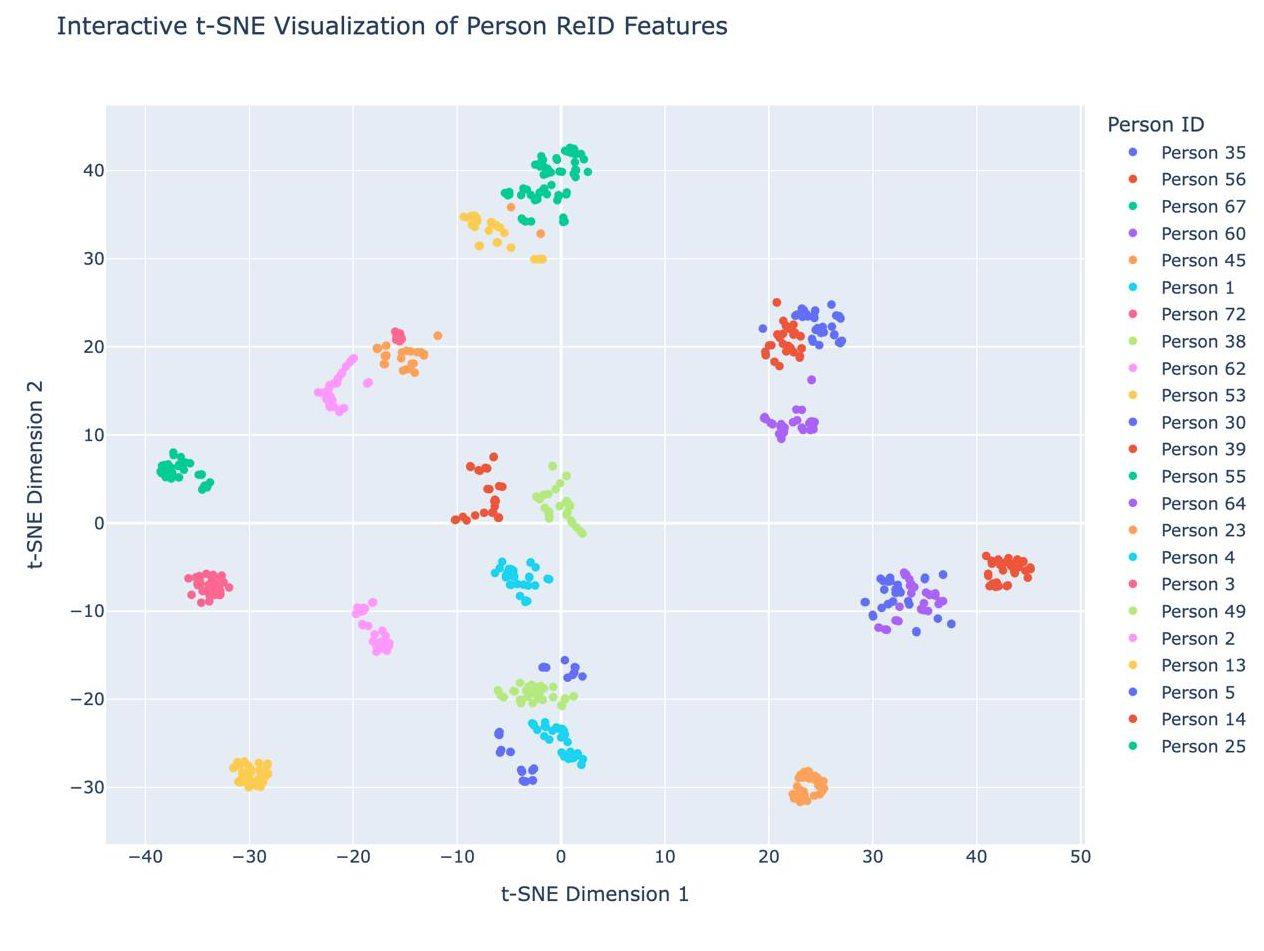
\includegraphics[width=0.8\textwidth]{pictures/tsne_inter_reid.jpeg}
    \caption{t-SNE projection of OSNet appearance features for multiple individuals. The distinct clustering for each person (indicated by color) demonstrates the feature space's discriminative power, enabling effective re-identification for post-processing tasks.}
    \label{fig:tsne_reid}
\end{figure}

For now, this basic visual ReID approach is employed without additional complex heuristics for the intra-camera ID switch correction, relying on the strength of the feature embeddings. Future work could explore incorporating motion continuity or short-term spatio-temporal predictions as additional cues to further refine the re-linking decisions.



























\subsection{Post-processing Heuristics}

Despite using state-of-the-art models (YOLOv12 for detection, BoT-SORT for tracking, and OSNet for ReID) for Single-Camera Multiple Object Tracking (MOT), online processing introduces challenges requiring post-processing. In particular, the Tracking by Detection (TBD) paradigm can produce erroneous tracks, known as \textit{phantom tracks}, due to detection misses.

\paragraph{Phantom Tracks}
In the TBD paradigm with online processing, phantom tracks arise when the tracker compensates for missed detections by predicting bounding boxes based on the motion model. Let a track for object $A$ be represented as a sequence of bounding boxes $\mathcal{T}_A = \{b_t = (x_t, y_t, w_t, h_t) \mid t = 1, \dots, T\}$, where $b_t$ is the bounding box at frame $t$, defined by center coordinates $(x_t, y_t)$, width $w_t$, and height $h_t$. The track is confirmed by detections up to frame $T_d \leq T$, where $T_d$ is the last frame with a detection from YOLOv12.

For frames $t > T_d$, if YOLOv12 fails to detect object $A$, the tracker uses a motion model (e.g., Kalman filter) to predict $b_t$:
\[
b_t = f_{\text{motion}}(b_{t-1}, v_{t-1}, \Sigma_{t-1}),
\]
where $f_{\text{motion}}$ is the motion prediction function, $v_{t-1}$ is the estimated velocity, and $\Sigma_{t-1}$ is the uncertainty covariance, which grows with time. As $t - T_d$ increases, $\Sigma_t$ expands, causing the predicted box $b_t$ to grow larger and less reliable, forming a phantom track. This is problematic if object $A$ has left the frame or remains occluded for many frames (i.e., $t - T_d > \tau$, where $\tau$ is the tracker's memory threshold).

\paragraph{Solution}
To eliminate phantom tracks, we apply a post-processing heuristic that terminates tracks at the last detection-confirmed frame. Formally, for track $\mathcal{T}_A$, we retain only the subsequence $\mathcal{T}_A' = \{b_t \mid t \leq T_d\}$, discarding predicted boxes for $t > T_d$. This ensures that tracks are anchored to verified detections, preventing exploding bounding boxes.


\paragraph{Manikin Misclassification}
Another disadvantage of using TBD is highly reliance of detection model outputs. For instance, YOLOv12, for some reason, very confidently (conf. about 0.9), classify makings are people.
Formally model assign high-confidence detections to static objects, initiating tracks $\mathcal{T}_i = \{b_t = (x_t, y_t, w_t, h_t) \mid t = 1, \dots, T\}$ for object $i$, where $b_t$ is the bounding box at frame $t$ with center $(x_t, y_t)$, width $w_t$, and height $h_t$. It leads to unnecessary, false tracks, which will mess up our further ReID and data analysis. To handle it I propose the movement statistics heuristic. 

Unlike moving objects, manikins show minimal displacement, causing the tracker (BoT-SORT) to maintain such unnecessary tracks.

To quantify movement, we compute the spatial boundaries of track $\mathcal{T}_i$ over its observation history:
\[
B_i = \left( \min_t x_t - \frac{w_t}{2}, \max_t x_t + \frac{w_t}{2}, \min_t y_t - \frac{h_t}{2}, \max_t y_t + \frac{h_t}{2} \right),
\]
defining the bounding rectangle $[x_{\min}, x_{\max}, y_{\min}, y_{\max}]$. We then calculate the average bounding box size for track $i$:
\[
\bar{w}_i = \frac{1}{T} \sum_{t=1}^T w_t, \quad \bar{h}_i = \frac{1}{T} \sum_{t=1}^T h_t.
\]
The normalized movement range is:
\[
\Delta x_i = \frac{x_{\max} - x_{\min}}{\bar{w}_i}, \quad \Delta y_i = \frac{y_{\max} - y_{\min}}{\bar{h}_i}.
\]
A static object (e.g., manikin) has low $\Delta x_i$ and $\Delta y_i$ (e.g., $\Delta x_i, \Delta y_i < \theta$), where $\theta$ is an empirically determined threshold (e.g., $\theta = 2$, meaning the object moves less than twice its average box size).


\paragraph{Solution}
To eliminate manikin tracks, we apply a post-processing heuristic that filters tracks based on their normalized movement range. For each track $\mathcal{T}_i$, if $\max(\Delta x_i, \Delta y_i) < \theta$, the track is classified as static and removed. This approach ensures only track with noticeable movement (likely people), reducing false positives from static objects (likely manikin)

\begin{figure}[h]
    \centering
    \begin{minipage}{0.45\textwidth}
        \centering
        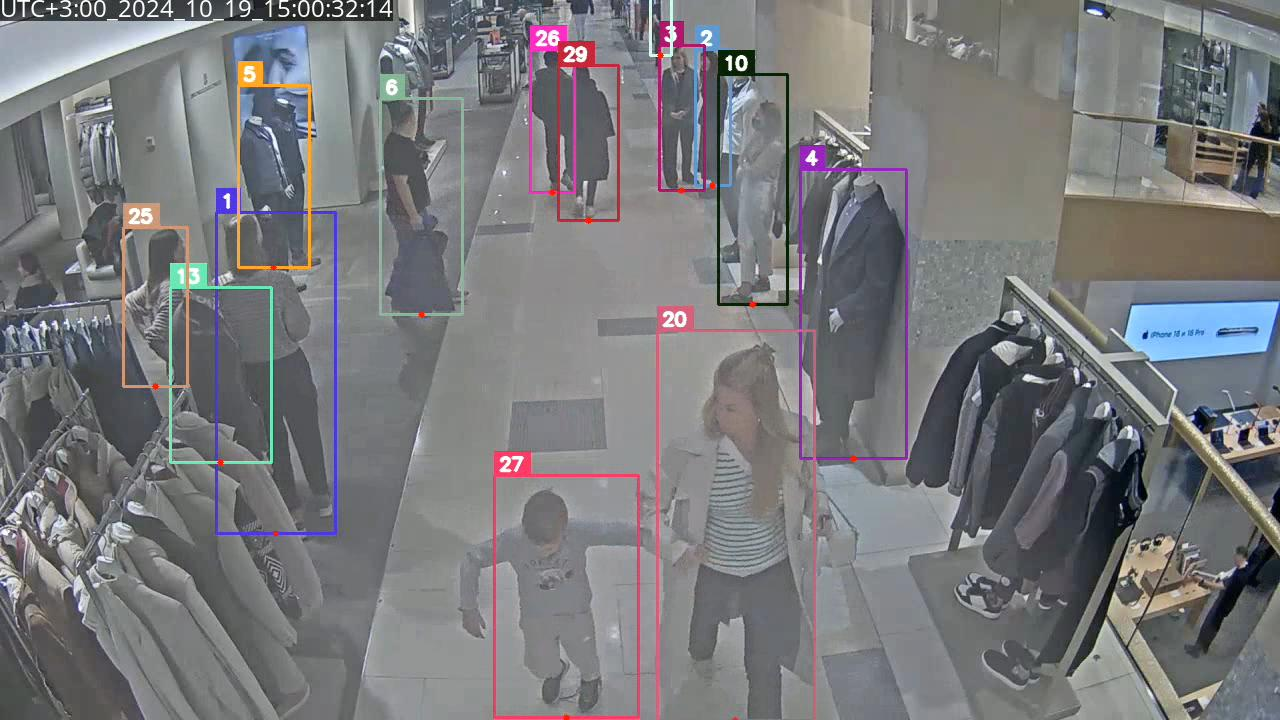
\includegraphics[width=\linewidth]{pictures/manik_a.jpeg}
        \caption{Result of Single-Camera MOT Pipeline work before post-processing heuristics.}
        \label{fig:manik_a}
    \end{minipage}
    \begin{minipage}{0.45\textwidth}
        \centering
        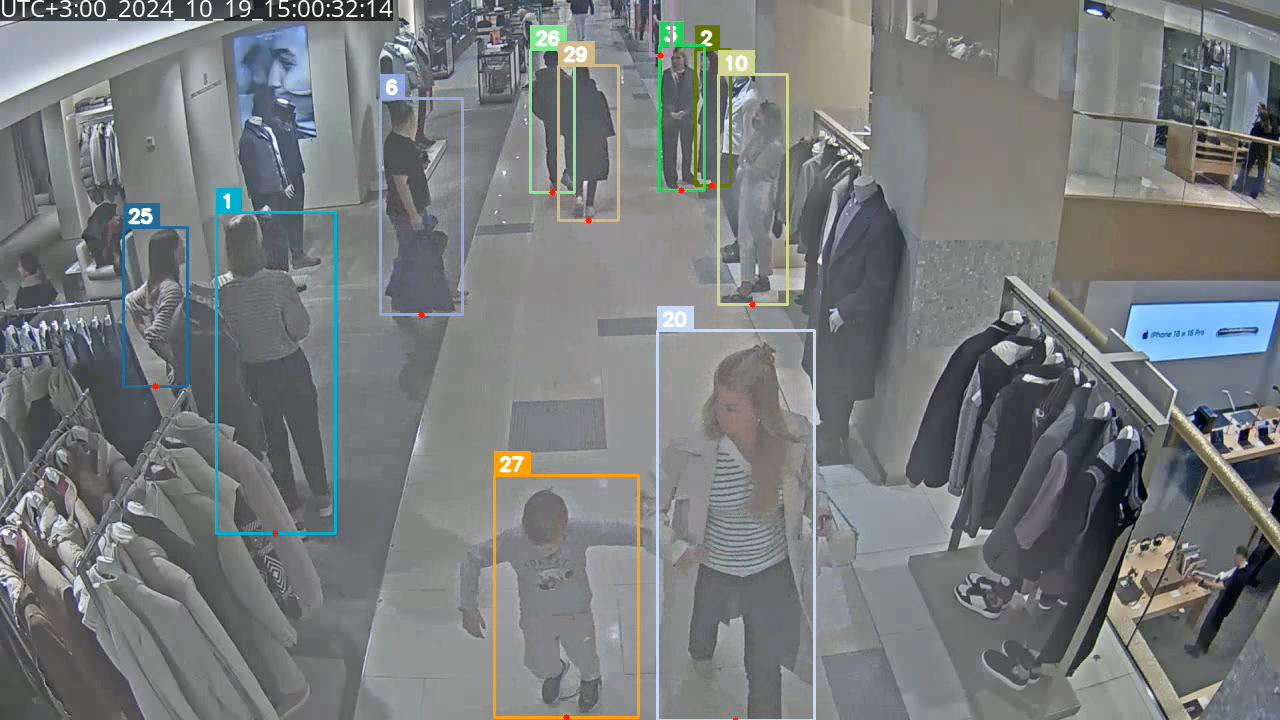
\includegraphics[width=\linewidth]{pictures/manik_b.jpeg}
        \caption{Result of Single-Camera MOT Pipeline work after post-processing heuristics.}
        \label{fig:manik_b}
    \end{minipage}
\end{figure}


\paragraph{Additional Cleanup Heuristics}
To further enhance track reliability, we apply the following minor heuristics:
\begin{enumerate}
    \item \textbf{Minimum Track Length}: Tracks with fewer than $\tau_{\text{min}}$ frames (e.g., $\tau_{\text{min}} = 20$, less than a second at 30 FPS) are removed. Formally, for track $\mathcal{T}_i$ with length $T_i$, if $T_i < \tau_{\text{min}}$, the track is discarded, as short tracks provide insufficient information for meaningful analysis.
  
    \item \textbf{Non-Confirmed Frames Threshold}: Tracks with a high proportion of non-confirmed (tracker-generated) frames are unreliable, risking identity switches and ReID errors. Let $T_{i,\text{det}}$ be the number of detection-confirmed frames in $\mathcal{T}_i$, and define the non-confirmed ratio as $r_i = \frac{T_i - T_{i,\text{det}}}{T_i}$. If $r_i > \phi$ (e.g., $\phi = 0.8$), the track is removed to prevent propagation of unreliable predictions.
\end{enumerate}

\section{Cross-Camera Person Re-identification}

\subsection{Attempts of Using Appearance-Only Approach}

Our initial approach to solving the Cross-Camera Person Re-identification (ReID) problem employed an appearance-only strategy, utilizing a gallery-query framework as reviewed in \cite{Specker-ReID}. As was discussed above this method relies on visual features extracted from cropped images to match identities across cameras.

Below, we detail the implementation, formalize the matching process, evaluate its performance, and discuss its limitations, which prompted the adoption spatiotemporal cues.

\subsubsection{Implementation}

Following the single-camera MOT pipeline (Section~\ref{subsec:sigle-camera-formalization}), each camera $C_m \in \mathcal{C}$ produces a set of tracklets $\mathcal{T}_m = \{ T_m^1, T_m^2, \ldots, T_m^{J_m} \}$, where each tracklet $T_m^j = (id_m^j, \mathbf{x}_{a:b}^{m,j}, \mathbf{f}_{a:b}^{m,j})$ includes a local ID, state sequence $\mathbf{x}_{a:b}^{m,j} \in (\mathbb{R}^6)^{b-a+1}$, and appearance feature sequence $\mathbf{f}_{a:b}^{m,j} \in (\mathbb{R}^{512})^{b-a+1}$ generated by ReID Model (e.g. OSNet). To perform cross-camera matching, we adopt a gallery-query framework where tracklets from one camera (query) are compared against tracklets from other cameras (gallery).

For each tracklet $T_m^j$, we extract crops from bounding boxes $\mathbf{x}_k^{m,j}$ using some heuristic sampling and process them with ReID model to obtain feature embeddings $\mathbf{f}_k^{m,j}$. To reduce computational complexity, we aggregate features within a tracklet by averaging \cite{Specker-ReID}:
\begin{equation}
\bar{\mathbf{f}}^{m,j} = \frac{1}{b-a+1} \sum_{k=a}^b \mathbf{f}_k^{m,j},
\end{equation}
where $\bar{\mathbf{f}}^{m,j} \in \mathbb{R}^{512}$ represents the average feature vector for tracklet $T_m^j$. We compute pairwise similarities between tracklets $T_m^j$ and $T_n^i$ from cameras $C_m$ and $C_n$ using cosine similarity \textit{(or other similarity metric, depending on our discriminative model, for OSNet it is cosine)}:

\begin{equation}
s(\bar{\mathbf{f}}^{m,j}, \bar{\mathbf{f}}^{n,i}) = \frac{\bar{\mathbf{f}}^{m,j} \cdot \bar{\mathbf{f}}^{n,i}}{\|\bar{\mathbf{f}}^{m,j}\|_2 \|\bar{\mathbf{f}}^{n,i}\|_2},
\end{equation}

where $s \in [-1, 1]$. A match is confirmed if $s > \theta_{\text{appearance}}$, with $\theta_{\text{appearance}} = 0.85$ determined empirically. The TorchReID library facilitates efficient feature extraction and integration with OSNet, streamlining the process.

We tested multiple ReID models, including OSNet and ResNet-based architectures, as reviewed in \cite{Specker-ReID}. Matches were assigned using a greedy algorithm, selecting the highest similarity pairs above the threshold while ensuring each tracklet is assigned to at most one global tracklet $T^j_{\text{global}} \in \mathcal{T}_{\text{global}}$, as defined in Section~\ref{subsec:sigle-camera-formalization}.


\begin{figure}[h]
    \centering
    \begin{minipage}{0.4\textwidth}
        \centering
        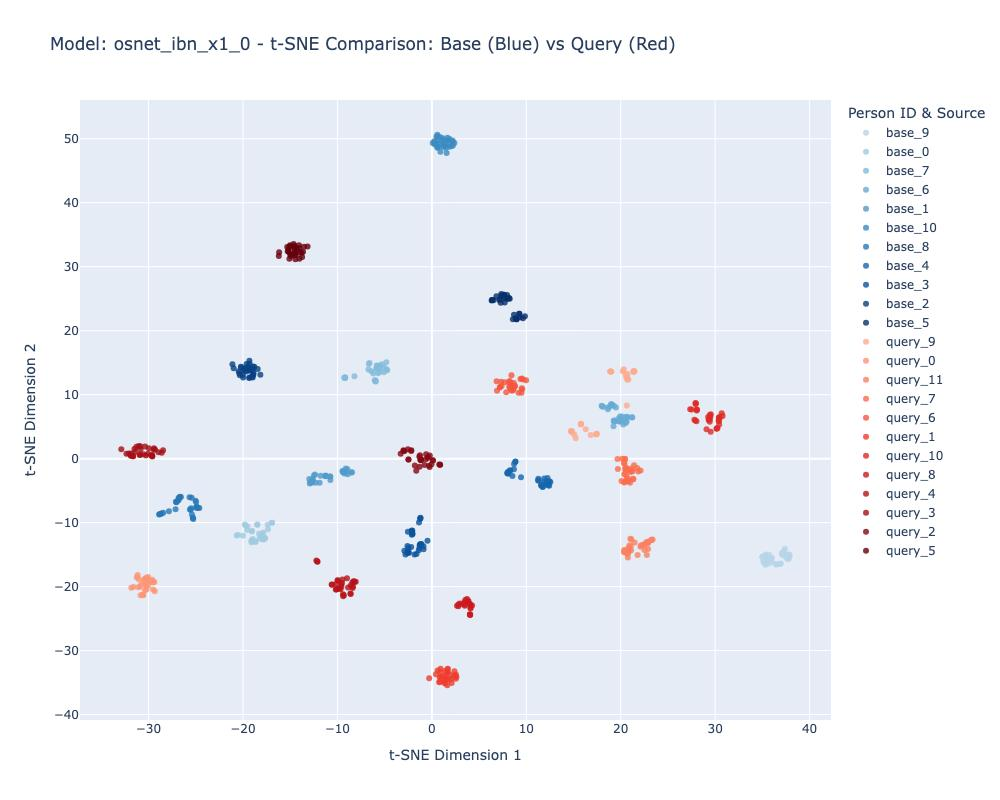
\includegraphics[width=\linewidth]{pictures/tsne_osnet.jpeg}
        \caption{t-SNE projection clustering of appearance only feature representative, OSNet results.}
        \label{fig:tsne_osnet}
    \end{minipage}
    \begin{minipage}{0.4\textwidth}
        \centering
        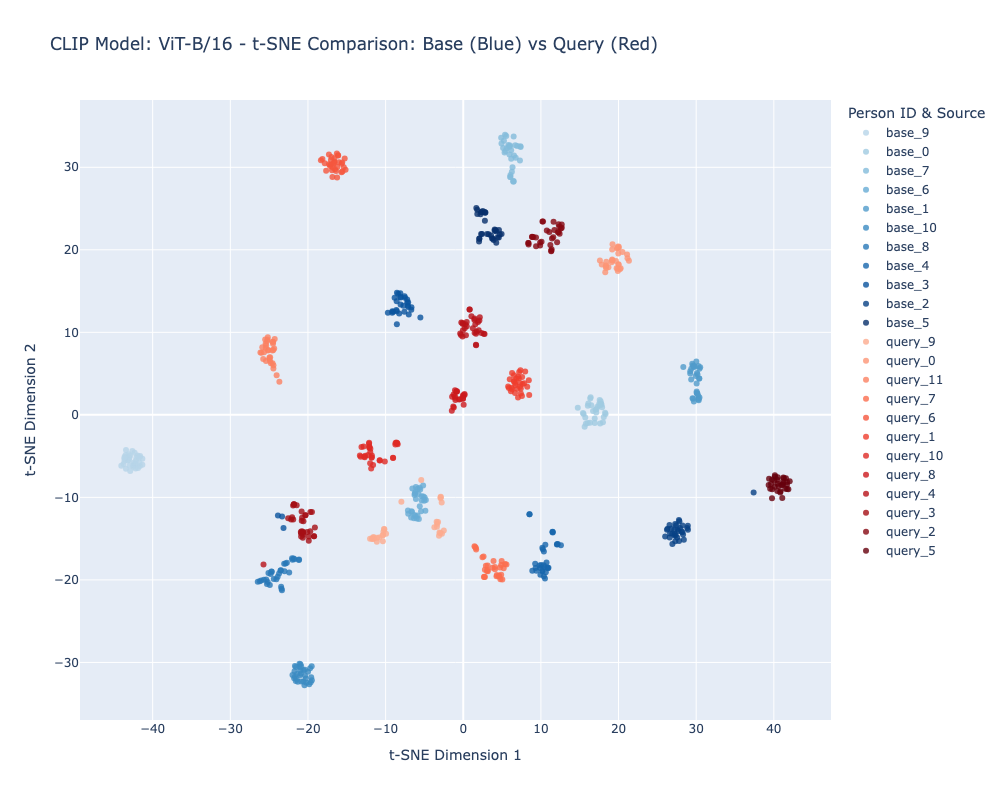
\includegraphics[width=\linewidth]{pictures/tsne_clip.png}
        \caption{t-SNE projection clustering of appearance only feature representative, CLIP results.}
        \label{fig:tsne_clip}
    \end{minipage}
\end{figure}

\subsubsection{Formal Matching Objective}

The objective is to group camera-specific tracklets into global tracklets $\mathcal{T}_{\text{global}}$ by maximizing the total similarity across matched pairs:
\begin{equation}
\mathcal{T}_{\text{global}}^* = \arg\max_{\mathcal{T}_{\text{global}}} \sum_{T^j_{\text{global}}} \sum_{(T_m^a, T_n^b) \in T^j_{\text{global}}} s(\bar{\mathbf{f}}^{m,a}, \bar{\mathbf{f}}^{n,b}),
\end{equation}
subject to the constraint that each tracklet $T_m^j$ belongs to exactly one global tracklet. This optimization assumes that high similarity scores indicate the same person, leveraging the feature space $\mathcal{F} = \mathbb{R}^{512}$ defined in Section~\ref{subsec:sigle-camera-formalization}.


\subsubsection{Performance and Limitations}

The appearance-only approach was evaluated using a t-SNE visualization of the feature embeddings $\bar{\mathbf{f}}^{m,j}$ across cameras (Figures ~\ref{fig:tsne_clip}\ref{fig:tsne_osnet}), revealing poor clustering of same-person identities. Quantitative evaluation using the IDF1 metric showed low identity consistency, indicating frequent mismatches. The key limitations are:
\begin{itemize}
    \item \textbf{Limited Observation Duration}: People in mall are typically visible for couple of seconds only per camera, resulting in sparse feature sequences $\mathbf{f}_{a:b}^{m,j}$. This limits the informativeness of the aggregated feature $\bar{\mathbf{f}}^{m,j}$, as it captures only few pose and angle variations.
    \item \textbf{High Appearance Variability}: Differences in camera angles, lighting, and clothing visibility cause significant feature divergence. For instance, a person may appear in a black jacket from behind in camera $C_m$ but with a white shirt visible from the front in camera $C_n$, yielding low similarity scores despite identical identity.
    \item \textbf{Computational Inefficiency}: Extracting features for person (we use 32 images gallery) take a while, especially while using CLIP models.
\end{itemize}
These issues led to suboptimal IDF1 scores and motivated a shift to alternative methods.

\subsection{Creating a Homography}
Homography provides a geometric mapping from each camera's view to a common reference plane, in this case the floor of a retail space. This allows pixel coordinates from any camera to be transformed into a shared "real-world" coordinate system on that plane. This global representation is essential for determining if individuals detected by different cameras are in the same physical location at the same time, a key component of my spatiotemporal constraints.

\paragraph{Intuitive Explanation}
Imagine you have several photos of the same tiled floor, each taken from a different camera angle. For each camera, a homography acts like a specific set of instructions that can warp its photo so that the tiles in it align perfectly with a master "bird's-eye view" map of that floor. To figure out these instructions for one camera, we need to identify several corresponding points (e.g., corners of tiles) that are in that camera's view and whose locations are known on the master floor map. Once you have enough of these "landmark" pairs (at least four, with no three in a straight line) for a camera, you can define its unique transformation to the master floor map.

\paragraph{Mathematical Formalism}
A homography is a projective transformation represented by a $3 \times 3$ matrix. (Note: The `pmatrix` environment used below requires the `amsmath` package).
\begin{enumerate}
    \item \textbf{Homogeneous Coordinates}: To handle projective transformations elegantly, 2D points $(x, y)$ are represented in homogeneous coordinates as 3D vectors $\mathbf{p} = [x, y, 1]^T$.

    \item \textbf{The Homography Equation}: In this work, a homography primarily maps points from a camera $C_m$'s image plane to a common real-world plane (the global floor plane $\mathcal{G} = \mathbb{R}^2$). Each camera $C_m$ is associated with a homography matrix $H_m \in \mathbb{R}^{3 \times 3}$ such that if $\mathbf{p}_m = [x_m, y_m, 1]^T$ are the homogeneous pixel coordinates of a point on the floor in camera $C_m$, its corresponding coordinates $\mathbf{g} = [x_g, y_g, 1]^T$ on the global floor plane are given by:
    $$\lambda_g \mathbf{g} = H_m \mathbf{p}_m$$
    where $\lambda_g$ is a non-zero scale factor. The matrix $H_m$ has the form:
    $$H_m = \begin{pmatrix} h_{11} & h_{12} & h_{13} \\ h_{21} & h_{22} & h_{23} \\ h_{31} & h_{32} & h_{33} \end{pmatrix}$$
    To find the corresponding pixel coordinates $\mathbf{p}_n$ in another camera $C_n$ for the point $\mathbf{p}_m$ from camera $C_m$ (assuming both represent the same physical point on the floor which is visible from both cameras), we first map $\mathbf{p}_m$ to the global plane to get $\mathbf{g}$ using $H_m$. Then, we reproject $\mathbf{g}$ from the global plane back to camera $C_n$'s image plane using the inverse of its homography, $H_n^{-1}$:
    $$\lambda_n \mathbf{p}_n = H_n^{-1} \mathbf{g}$$
    Substituting $\mathbf{g}$ (and ignoring scale factors for simplicity in the composite notation) gives the effective transformation from camera $C_m$ to camera $C_n$ via the global plane as $H_{m \to n} \propto H_n^{-1} H_m$. This approach of using an intermediary global plane is advantageous for robustly aligning multiple camera views. However, for the primary task of determining if two detections (one from each camera) are spatially proximate, explicitly reprojecting points from one camera view to another is often unnecessary. Instead, proximity can be assessed by directly comparing their transformed real-world coordinates on the global plane, as detailed in the application section.

    \item \textbf{Solving for H (Direct Linear Transform - DLT)}:
    A homography has 8 degrees of freedom (as it's defined up to a scale factor). Thus, at least four pairs of corresponding points (pixel coordinates in camera $C_m$ and their known real-world coordinates on the global plane $\mathcal{G}$) are needed to solve for $H_m$. Each point pair $(x_m,y_m) \leftrightarrow (x_g,y_g)$ provides two linear equations in the elements of $H_m$:
        $$h_{11}x_m + h_{12}y_m + h_{13} - h_{31}x_m x_g - h_{32}y_m x_g - h_{33}x_g = 0$$
        $$h_{21}x_m + h_{22}y_m + h_{23} - h_{31}x_m y_g - h_{32}y_m y_g - h_{33}y_g = 0$$
    With $N \ge 4$ point pairs, these equations form a system $A \mathbf{h} = \mathbf{0}$, where $A$ is a $2N \times 9$ matrix and $\mathbf{h}$ is a $9 \times 1$ vector containing the elements of $H_m$. This system is solved using Singular Value Decomposition (SVD). The solution $\mathbf{h}$ is the last column of $V$ in the SVD $A = U \Sigma V^T$. Point coordinate normalization before DLT is crucial for numerical stability.
\end{enumerate}


\begin{figure}[H]
    \centering
    \begin{minipage}{0.48\linewidth}
        \centering
        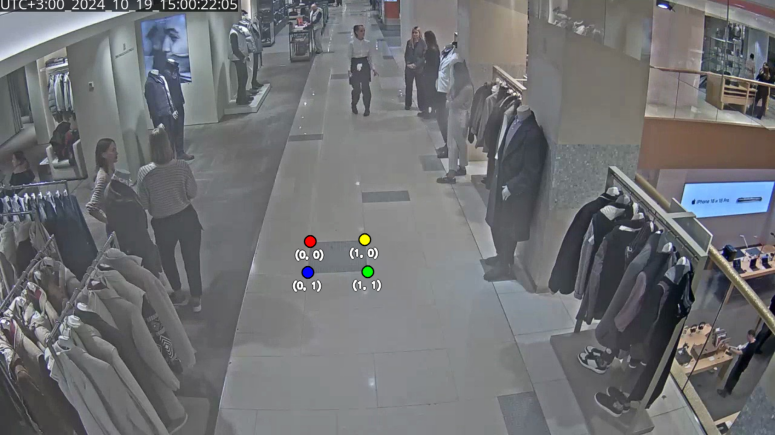
\includegraphics[width=\linewidth]{pictures/keypoints1.png} % Ensure this path is correct
    \end{minipage}
    \hfill % Separator between minipages
    \begin{minipage}{0.48\linewidth}
        \centering
        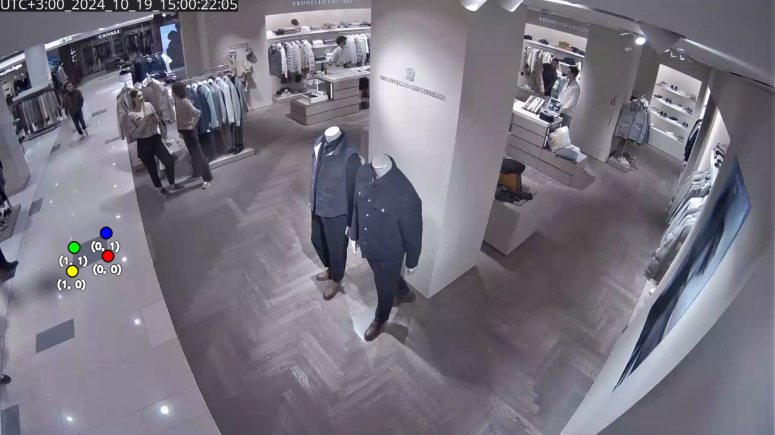
\includegraphics[width=\linewidth]{pictures/keypoints2.png} % Ensure this path is correct
    \end{minipage}
    \caption{Examples of corresponding points (colored dots representing corners of a central 1x1 meter reference tile) selected on the floor plane in Camera 1 (left) and Camera 2 (right) views, used for calculating their respective homography matrices to the global plane.}
    \label{fig:homography_points_pair}
\end{figure}

The alignment isn't perfect due to the camera's \textbf{fisheye distortion}. This type of optical distortion can be further treated using \textbf{lens distortion correction} techniques, typically derived from a camera calibration process which estimates the distortion parameters and allows for the image to be remapped to a rectilinear projection. I've tried to improve the accuracy of my homography mapping, especially trying to handle the fisheye problem by using more manually annotated points. For that, I used points located at the edges (not only on the central 1x1 meter tile) of the camera's shared views, manually annotating their real-world coordinates, taking as the basis the 1x1 tile which I know for sure is square. This is illustrated in Figure~\ref{fig:wide_homography_points_pair}. However, this approach brought no additional accuracy to the homography mapping itself. Therefore, I can conclude that for the purpose of homography estimation, using easily obtainable but well-aligned real-world points (like the corners of a central, known-square tile, as shown in Figure~\ref{fig:homography_points_pair}) is sufficient and possibly better than attempting to incorporate more widely distributed points whose real-world coordinates might be harder to ascertain with high precision, especially if underlying lens distortions are not separately corrected prior to homography calculation.

\begin{figure}[H]
    \centering
    \begin{minipage}{0.48\linewidth}
        \centering
        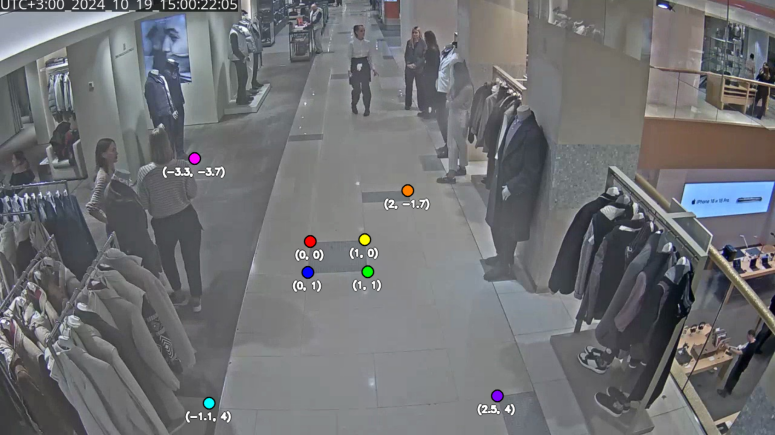
\includegraphics[width=\linewidth]{pictures/keypoints1_ext.png} % Ensure this path is correct
    \end{minipage}
    \hfill % Separator between minipages
    \begin{minipage}{0.48\linewidth}
        \centering
        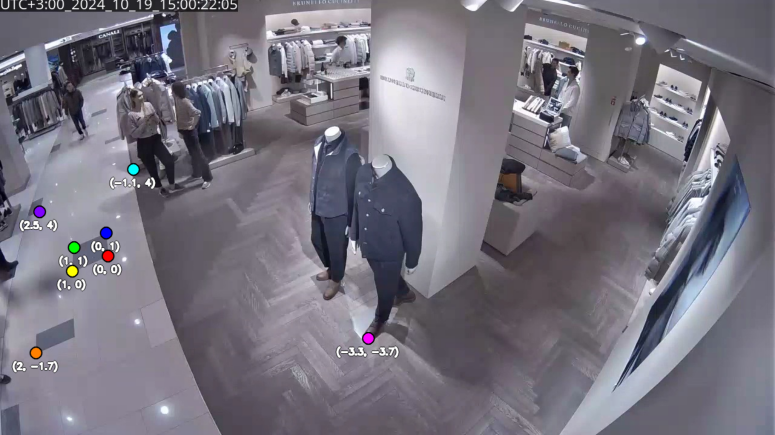
\includegraphics[width=\linewidth]{pictures/keypoints2_ext.png} % Ensure this path is correct
    \end{minipage}
    \caption{Attempt to improve homography accuracy using additional, widely distributed manually annotated points in Camera 1 (left) and Camera 2 (right), showing their annotated real-world coordinates.}
    \label{fig:wide_homography_points_pair}
\end{figure}

\subsubsection{Application in Cross-Camera ReID}
Once the homography $H_m$ (mapping camera $C_m$'s pixel coordinates to the global floor plane $\mathcal{G}$) is established for each camera, the floor position $(c_x, c_y)$ of a detected person (the center of the lower bounding line of their bounding box) in camera $C_m$ can be transformed to a global coordinate $\mathbf{g}_k^{m,j} = H_m ([c_x, c_y, 1]^T)$. These global coordinates, along with timestamps, form the basis for the spatiotemporal constraint in ReID: if two tracklets from different cameras, $T_m^j$ and $T_n^i$, have observations at frame $k$ (or very close in time $t_k^m \approx t_k^n$) such that their global positions $\mathbf{g}_k^{m,j}$ and $\mathbf{g}_k^{n,i}$ are nearby (e.g., $\|\mathbf{g}_k^{m,j} - \mathbf{g}_k^{n,i} \|_2 < \epsilon$), they are considered candidates for being the same person. This significantly prunes the search space for appearance-based matching. Figure~\ref{fig:projection_examples_pair} illustrates how known global coordinates can be projected onto different camera views using their respective inverse homographies ($H_m^{-1}$), demonstrating the alignment achieved. 


We utilize a \textbf{floor-based homography} because it establishes a geometric transformation that accurately maps points from a camera view to a global coordinate system $\mathcal{G}$ under the critical assumption that these points physically lie on the common floor plane. This approach simplifies the complex 3D problem of object localization to a more manageable 2D planar mapping. Consequently, when relating detected persons (who are 3D objects) to this floor plane, it is essential to use the \textbf{lower points of their bounding boxes} (e.g., the center of the bottom edge, approximating the feet's position). 

\begin{figure}[H]
    \centering
    \begin{minipage}{0.48\linewidth}
        \centering
        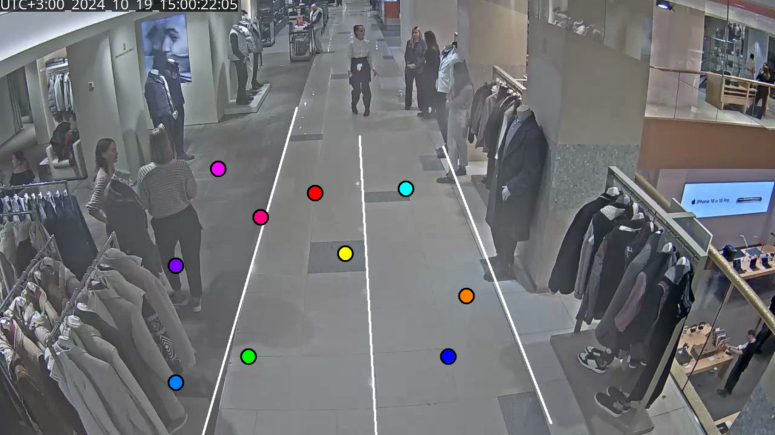
\includegraphics[width=\linewidth]{pictures/camer1_random.png} % Ensure this path is correct
    \end{minipage}
    \hfill % Separator between minipages
    \begin{minipage}{0.48\linewidth}
        \centering
        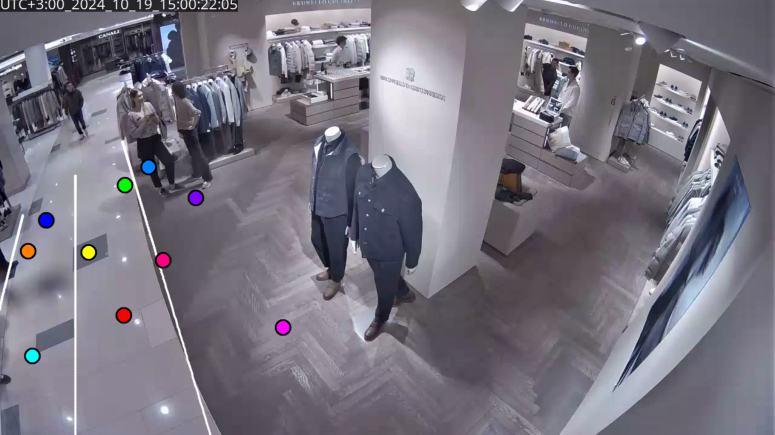
\includegraphics[width=\linewidth]{pictures/camer2_random.png} % Ensure this path is correct
    \end{minipage}
    \caption{Randomly chosen on first camera (left) points and supportive lines are reprojected to second camera (right) using their respective inverse homographies ($H_1^{-1}$ and $H_2^{-1}$).}
    \label{fig:projection_examples_pair}
\end{figure}


\subsection{Coordinate-based Matching}
\label{sec:coord_matching}
Following the homography transformation, for each detected identity $j$ from a camera $C_m$ at a specific frame $k$ with timestamp $t_k$, we possess its "real-world" shared coordinates on the global floor plane. These are derived from the center of its lower bounding box, approximating the feet's position, and denoted as $\mathbf{g}_k^{m,j} = (x_{\text{real},k}^{m,j}, y_{\text{real},k}^{m,j})$. Thus, a tracklet $T^{m,j}$ for identity $j$ from camera $C_m$ can be represented as a sequence of tuples: $T^{m,j} = \{ (k, \mathbf{b}_k^{m,j}, \mathbf{g}_k^{m,j}, t_k) \}_{k=k_{\text{start}}}^{k_{\text{end}}}$, where $\mathbf{b}_k^{m,j}$ represents the bounding box coordinates in the image plane.

The primary goal is, for each query tracklet $T_q$ (an identity from a specific camera), to find a matching tracklet from a set of candidate tracklets $T_c$ (from a base camera) or to establish its uniqueness as a new global identity. It is worth noting that for certain camera views or specific regions within them, we can assume a negligible probability of new identities appearing if there are no physical entrances to that monitored area.

\subsubsection{Initial Approach: Total Best Match}
My initial matching strategy was based on finding the "total best match" at each concurrent timestamp. For a detection within the query tracklet $T_q$ at timestamp $t$, its real-world coordinates $\mathbf{g}_{q,t}$ were compared against the real-world coordinates $\mathbf{g}_{c,t}$ of all active detections in candidate tracklets $T_c$ at the same timestamp $t$. The Euclidean distance $D(\mathbf{g}_{q,t}, \mathbf{g}_{c,t}) = \| \mathbf{g}_{q,t} - \mathbf{g}_{c,t} \|_2$ was calculated. If the minimum distance found for a candidate $T_c$ was below a predefined threshold $\theta_{dist}$, an identity link was concluded. Otherwise, the query tracklet $T_q$ was assigned a new, unique global ID. While simple and reasonably effective in many scenarios, this approach often failed in complex situations because it disregarded the broader temporal information contained within the tracklets, focusing only on the single best-matched frame.

\subsubsection{Improved Score-Based Matching}
To address the limitations of the initial method, a more comprehensive score function was defined to evaluate the affinity between a detection $d_1 = (\mathbf{g}_1, t_1)$ from one tracklet and $d_2 = (\mathbf{g}_2, t_2)$ from another. This score, where lower values indicate better similarity, was defined as:
$$ S_{pair}(d_1, d_2) = 0.1 \cdot L_{time}(t_1, t_2) \cdot D_{Euclidean}(\mathbf{g}_1, \mathbf{g}_2) $$
The components are:
\begin{itemize}
    \item Time loss: $L_{time}(t_1, t_2) = |t_1 - t_2|$ if $|t_1 - t_2| < \tau_{time}$ (e.g., $\tau_{time} = 10$ frames), and $L_{time}(t_1, t_2) = \infty$ otherwise.
    \item Distance difference: $D_{Euclidean}(\mathbf{g}_1, \mathbf{g}_2) = \| \mathbf{g}_1 - \mathbf{g}_2 \|_2$.
\end{itemize}
Using this score, for each detection $d_{q,k}$ in a query tracklet $T_q$ (at frame $k$ with timestamp $t_k$), and for each candidate tracklet $T_c$:
\begin{enumerate}
    \item We computed $S_{pair}(d_{q,k}, d_{c,k'})$ for all detections $d_{c,k'}$ in $T_c$ where the timestamp $t_{k'}$ was within a small temporal window around $t_k$ (e.g., $\pm 5$ frames).
    \item The minimum score found within this window for $T_c$ (denoted $S^*_{k,c}$) was considered the best local match for $d_{q,k}$ with $T_c$.
    \item If $S^*_{k,c}$ was beneath a certain threshold $\theta_{local\_score}$, it was added to a cumulative sum $S_{total}(T_q, T_c)$ for that candidate tracklet $T_c$. This thresholding step avoided penalizing comparisons for detections not yet simultaneously visible or significantly misaligned.
    \item The candidate tracklet $T_c$ with the lowest overall $S_{total}(T_q, T_c)$ was chosen as the best match. If it's score is beneath $\theta_{global\_score}$, otherwise the query tracklet $T_q$ was assigned a new, unique global ID
\end{enumerate}
This refined approach provided more robustness but still exhibited some misses in challenging scenarios.

\subsubsection{Final Matching Approach: Exponential Loss and Refined Scoring}
A key observation was that the Euclidean distance, growing linearly, might not be optimal. Small differences in real-world coordinates can often be attributed to homography imperfections and should ideally be down-weighted, whereas larger distances (e.g., $>1$ meter) are highly significant, especially in dense scenes. Simply thresholding the distance to binary values (0 or $\infty$) is also suboptimal. Therefore, a non-linear mapping for the distance was proposed using an exponential-like function to create a similarity score where larger values indicate better similarity:
$$ S_{dist}(\mathbf{g}_1, \mathbf{g}_2) = a \cdot \exp(-b \cdot \| \mathbf{g}_1 - \mathbf{g}_2 \|_2) $$
Satisfactory performance was achieved with parameters $a = 10$ and $b = 2.5$.

With advancements in time synchronization across cameras, perfect timestamp matching ($t_1 = t_2$) became achievable, allowing the "time\_loss" component to be removed from the score. The resulting similarity score for a pair of detections, $d_{q,k}$ from query tracklet $T_q$ and $d_{c,k}$ from candidate tracklet $T_c$ at the same frame/timestamp $k$, is $S_{k}(d_{q,k}, d_{c,k}) = S_{dist}(\mathbf{g}_{q,k}, \mathbf{g}_{c,k}).$


The overall matching score between a query tracklet $T_q$ and a candidate tracklet $T_c$ is then calculated as the sum of these individual similarity scores $S_k$ across all co-occurring frames, normalized by the number of frames where $S_k$ exceeded a minimum contribution threshold $\theta_{contrib}$ (e.g., $\theta_{contrib} = 1$). Let $K_{overlap}$ be the set of frames where both $T_q$ and $T_c$ have detections, and $N_{contrib} = |\{k \in K_{overlap} \mid S_k > \theta_{contrib}\}|$. The normalized total score is:
$$ S_{total}(T_q, T_c) = \frac{1}{N_{contrib}} \sum_{k \in K_{overlap}, S_k > \theta_{contrib}} S_k $$
assuming $N_{contrib} > 0$.

The decision logic based on this normalized score $S_{total}$ (where larger is better) is as follows:
\begin{enumerate}
    \item Let $S_{best}$ be the highest score achieved by $T_q$ with any candidate $T_c$, and $S_{next\_best}$ be the second-highest score.
    \item If $S_{best} > \theta_{global}$ (e.g., $\theta_{global} = 1000$) AND $S_{next\_best} < S_{best} / 2$, then $T_q$ is confidently linked to the candidate tracklet corresponding to $S_{best}$.
    \item If $S_{best} < \theta_{global}$, $T_q$ is considered a unique identity.
    \item If $S_{best} > \theta_{global}$ but there are several candidate tracklets with high scores (e.g., all candidates $T_c$ whose scores $S_{total}(T_q, T_c) \ge S_{best} / 2$, it unlikely to have $k > 3$ such candidates in realistic scenarios), a visual-based ReID model is employed as a tie-breaker. Appearance features are extracted for these top-$k$ candidates and the query tracklet. Similarity scores are computed (e.g., cosine similarity), and a final decision can be made by combining the homography-based score and the appearance-based score (e.g., by multiplication) to determine the ultimate match.
\end{enumerate}
This multi-stage approach, leveraging robust spatiotemporal matching with an exponential loss function and falling back to appearance features for ambiguous cases, has proven to be stable and highly accurate, leading to an efficient solution for the cross-camera ReID problem.

\subsubsection{Cross-View Feature Aggregation for Robust Appearance ReID}

This coordinate-based matching across cameras allows for the association of identities, effectively providing multiple, different-angle views of the same individual as they move through areas covered by homography-linked cameras. This aggregated visual information can be used to create a more comprehensive appearance-based representation for each person. By combining crops from these diverse viewpoints, the robustness of visual ReID can be significantly improved. This enhanced appearance model can then be employed as a more effective, albeit still last-resort, matching approach for cameras where homography information is unavailable or inapplicable—for instance, cameras with unique, non-overlapping views that cannot be spatially linked to the main network.





\subsection{Homography-based ReID Results}


\begin{figure}[H]
    \centering
    \begin{minipage}{0.48\linewidth}
        \centering
        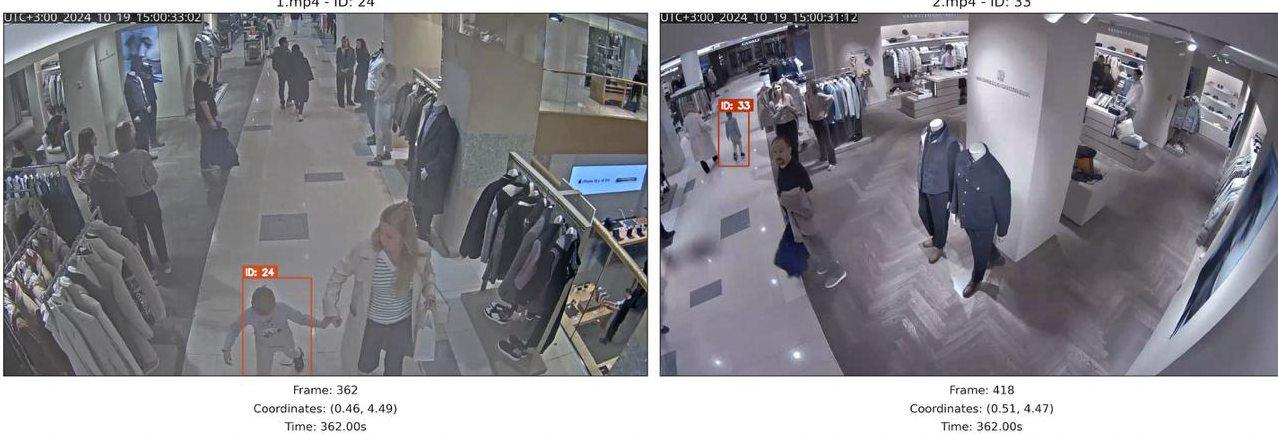
\includegraphics[width=\linewidth]{pictures/demo_reid1.jpeg} % Ensure this path is correct
        % \caption*{(a) demo_reid1.jpeg} % Optional sub-label
    \end{minipage}
    \hfill % Separator between minipages
    \begin{minipage}{0.48\linewidth}
        \centering
        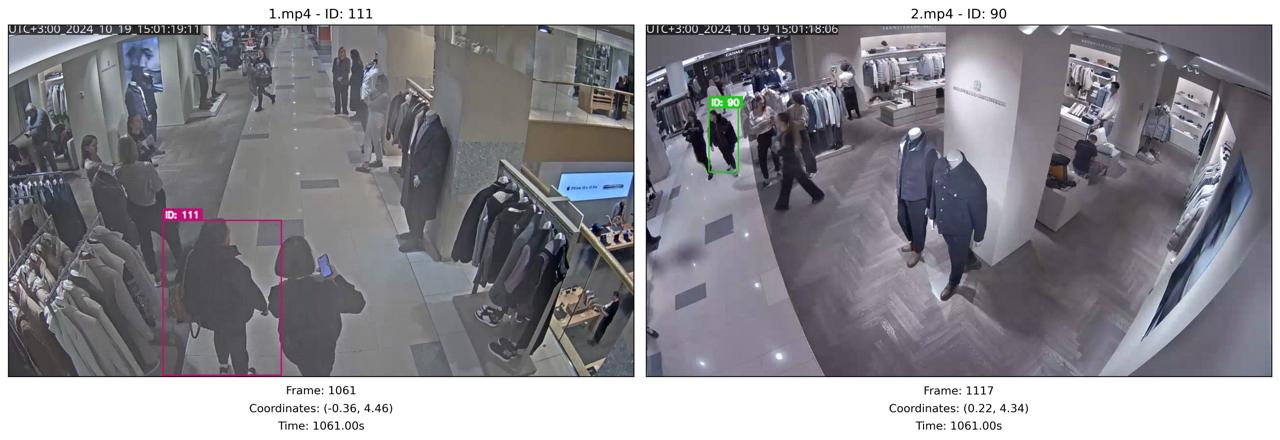
\includegraphics[width=\linewidth]{pictures/demo_reid3.jpeg} % Ensure this path is correct
        % \caption*{(b) demo_reid3.jpeg} % Optional sub-label
    \end{minipage}
    \caption{Examples of successful ReID using coordinate-based matching in scenarios with relatively clear views (left: ID 24 $\leftrightarrow$ ID 33; right: ID 111 $\leftrightarrow$ ID 90), where appearance-based methods might also succeed.}
    \label{fig:reid_demos_good_appearance}
\end{figure}

\begin{figure}[H]
    \centering
    \begin{minipage}{0.48\linewidth}
        \centering
        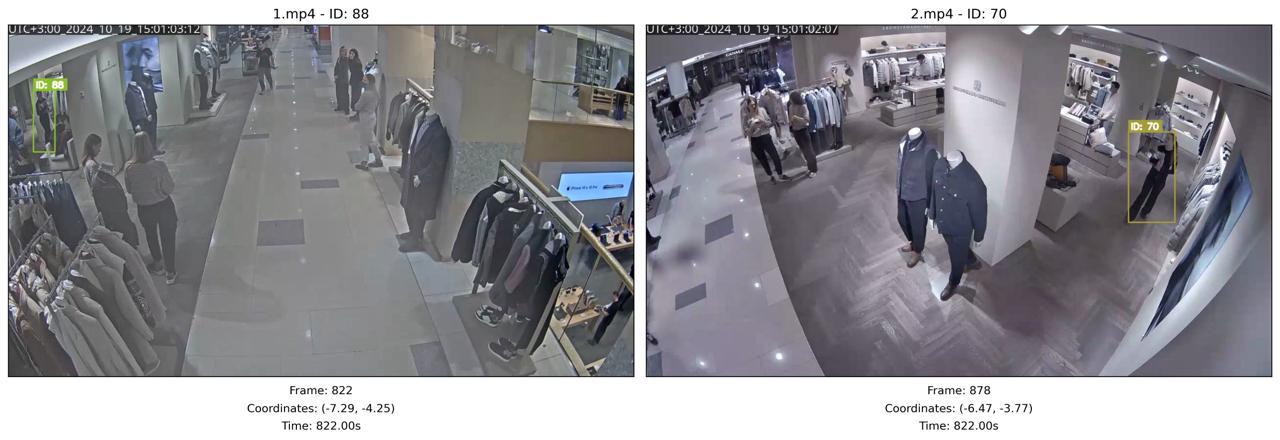
\includegraphics[width=\linewidth]{pictures/demo_reid2.jpeg} % Ensure this path is correct
        % \caption*{(a) demo_reid2.jpeg} % Optional sub-label
    \end{minipage}
    \hfill % Separator between minipages
    \begin{minipage}{0.48\linewidth}
        \centering
        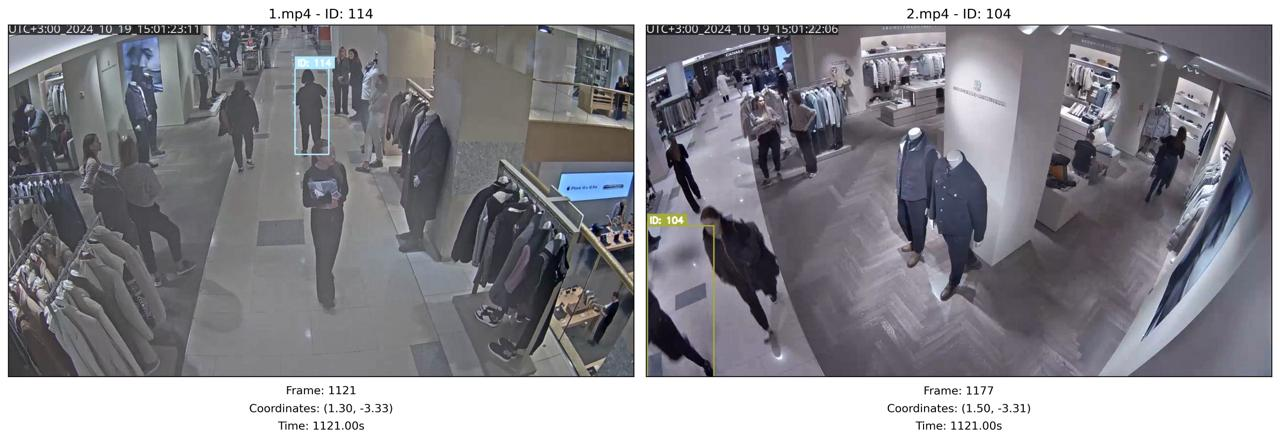
\includegraphics[width=\linewidth]{pictures/demo_reid4.jpeg} % Ensure this path is correct
        % \caption*{(b) demo_reid4.jpeg} % Optional sub-label
    \end{minipage}
    \caption{Demonstration of coordinate-based ReID robustness in challenging scenarios: matching with a very small, non-informative crop (left: ID 88 $\leftrightarrow$ ID 70), and matching with an incomplete human figure in the bounding box (right: ID 114 $\leftrightarrow$ ID 104).}
    \label{fig:reid_demos_challenging_appearance}
\end{figure}



The efficacy of this final spatiotemporal matching approach is demonstrated in Figures~\ref{fig:reid_demos_good_appearance} and \ref{fig:reid_demos_challenging_appearance}. For instance, in Figure~\ref{fig:reid_demos_good_appearance} (left image) and (right image), we observe proper matching of identities (ID 24 $\leftrightarrow$ ID 33 and ID 111 $\leftrightarrow$ ID 90, respectively). These cases, with relatively clear views, could theoretically also be resolved using robust appearance-based methods. However, the strength of the coordinate-based approach becomes particularly evident in more challenging scenarios. Figure~\ref{fig:reid_demos_challenging_appearance} (left image) shows successful matching (ID 88 $\leftrightarrow$ ID 70) despite one of the detections providing a very small and non-informative visual crop. Furthermore, Figure~\ref{fig:reid_demos_challenging_appearance} (right image) demonstrates the system's ability to link identities (ID 114 $\leftrightarrow$ ID 104) even when a bounding box does not capture a complete human figure, a situation where visual crop information would be highly unreliable or misleading for appearance-based ReID.


This multi-stage approach, leveraging robust spatiotemporal matching with an exponential loss function and falling back to appearance features for ambiguous cases, has proven to be stable and highly accurate, leading to an efficient solution for the cross-camera ReID problem.


\section{Further Research Directions}
While the developed system demonstrates excellent results there are several avenues for future research that could enhance its performance, automation, and applicability.

\subsection{Enhanced Camera Distortion Correction}

Currently our mapping (camera's coordinates to real-work ones), suffers from a fisheye distortion, presented in the camera feeds. Further research will address this problem using camera calibration to estimate and counteract the specific distortion parameters of each camera, leading to a more accurate reprojection of image points to the global floor plane and subsequently improving the precision of coordinate-based matching.

\subsection{Automated Homography Generation}

Currently, the establishment of homography relies on manually selected corresponding points between camera views and the global plane. Future work could focus on automating this process. This could involve developing algorithms to automatically detect stable and reliable key points, such as high-contrast corners of floor tiles or other salient static features within the retail environment. Successful automation would significantly reduce the manual setup required for new camera installations, making the system more scalable and easier to deploy without extensive per-camera calibration.

\subsection{Automatic Time Synchronization}

Although the current system assumes time-synchronized cameras, exploring methods for automatic time synchronization or fine-tuning synchronization could be beneficial. One potential approach could involve analyzing strong temporal cues from the video data itself. For instance, correlating the gait patterns of individuals observed simultaneously (or near-simultaneously based on initial rough synchronization) in the overlapping fields of view of different cameras could help to align frames with high precision. This would ensure that spatiotemporal constraints are applied to data that is truly concurrent.

\subsection{Advanced 3D Scene Representation via Multi-Layer Homography}

The current system employs a floor-based homography, mapping points to a single 2D plane. An interesting extension would be to explore pseudo-3D mapping techniques, such as the multi-layer homography proposed in Arsić et al. (2008)\cite{multi-layer-homography} , or concepts from view-centric tracking with homographic matching in dynamic UAV scenarios as seen in Ji et al. (2024) \cite{Homography-UAV} . This could involve projecting object detections onto multiple height layers, creating a richer spatial representation of the scene. Such a pseudo-3D approach might offer more robust localization and association, especially in scenarios with significant height differences or when dealing with objects not strictly on the floor plane, further enhancing Re-ID accuracy across cameras.


\subsection{Incorporating Spatial Priors for New Identity Plausibility and Gallery Management}

Future enhancements could involve leveraging semantic understanding of the retail space by segmenting camera views into zones based on the likelihood of new identities appearing (e.g., areas near entrances/exits versus internal walkways). This spatial prior could dynamically adjust Re-ID gallery sizes; for instance, tracklets appearing in zones with no external access would be strongly forced to match existing global IDs, reducing the search space and computational load. This approach could also refine single-camera tracking by informing the tracker that an identity reappearing in an exit-less internal segment is highly likely to be a previously observed one. This would create more robust constraints, especially for the cross-camera matching problem where queries from "must-match" zones would require association with a base identity, potentially improving overall system accuracy and efficiency.


\section{Conclusion}

This research has addressed the complex challenge of continuous multi-user tracking within retail environments by developing an innovative system focused on robust single-camera tracking and effective cross-camera re-identification (Re-ID). The primary objective was to generate comprehensive and accurate visitor trajectories across a network of static surveillance cameras, providing valuable data for retail analytics.

For single-camera tracking, we enhanced a state-of-the-art pipeline (YOLOv12, BoT-SORT, OSNet) through the introduction of tailored post-processing heuristics. These heuristics specifically targeted the mitigation of phantom tracks arising from prolonged occlusions and the misclassification of static objects like manikins, significantly improving the reliability and accuracy of individual camera tracklets. Furthermore, a post-processing Re-ID step was implemented to correct identity switches within a single camera's view that occurred after extended occlusions, leveraging an appearance-based query-gallery approach.

The core innovation of this work lies in our cross-camera Re-ID methodology. Recognizing the limitations of purely appearance-based approaches in dynamic retail settings with short observation windows and significant visual changes, we developed a robust spatiotemporal matching strategy. This strategy utilizes homography to transform detected person locations onto a common ground plane, enabling coordinate-based comparisons. A novel exponential loss function was introduced for similarity scoring between tracklets based on their real-world coordinates, which proved more effective than linear distance metrics in handling minor homography imperfections while strongly penalizing larger spatial discrepancies. This formed the basis of a multi-stage matching process where spatiotemporal constraints primarily guide Re-ID decisions, with aggregated appearance features from multiple confirmed views serving as a fallback mechanism for ambiguous cases or cameras without homographic linkage. Our results demonstrated that this approach can successfully re-identify individuals even with non-informative visual crops or incomplete detections, leading to stable and highly accurate cross-camera trajectory generation.

The developed system provides a significant step towards reliable, automated customer journey analysis in retail spaces. However, limitations exist, such as the current reliance on manually defined homography points and the potential impact of uncorrected lens distortion.

Future research, as outlined in Section 8, will focus on enhancing the system's automation and precision. Key directions include enhanced camera distortion correction, automated homography generation, automatic time synchronization refinement, exploring advanced 3D scene representations like multi-layer homography, and incorporating spatial priors for managing new identity plausibility. These advancements promise to further improve the system's robustness, scalability, and applicability in real-world retail environments.

\section*{Acknowledgments}

We would like to express our sincere gratitude to\textbf{ Gurbanov Nihad} for the insightful idea of utilizing coordinate-time features for cross-camera person re-identification (ReID). This contribution significantly enhanced the methodological framework of our work.

\begin{multicols}{2}
\small
\printbibliography
\end{multicols}
\end{document}
